\documentclass[12pt,a4paper,openany,final,twoside,longbibliography,hidelinks]{book}
\usepackage{acronym}
\usepackage[english]{babel}
\usepackage[utf8]{inputenc}
\usepackage[T1]{fontenc}
\usepackage{amsmath}
\usepackage{mathtools}
\usepackage{amsfonts}
\usepackage{amssymb}
\usepackage{bbold}
\usepackage{esdiff}
\usepackage[]{graphicx}
\usepackage[sort&compress,numbers]{natbib}
\bibliographystyle{unsrtnat}
% \bibliographystyle{aipnum4-2}
\usepackage{doi}
\renewcommand*{\bibfont}{\interlinepenalty 10000\relax}
\usepackage[defaultlines=2,all]{nowidow}
\usepackage{siunitx}
\sisetup{range-phrase=--}
\sisetup{range-units=single}
 
\usepackage[dvipsnames]{xcolor}
\usepackage{bm}
\usepackage{float}
\usepackage{verbatim}
\usepackage{afterpage}
\usepackage{microtype}
\usepackage[labelfont=bf]{caption}
\captionsetup[table]{position=above}
\usepackage{subfigure} 
\usepackage[onehalfspacing]{setspace}
\usepackage{blindtext} 
\numberwithin{equation}{section}
\usepackage{etoolbox}
\graphicspath{{./images/}}
\usepackage[]{geometry}
\usepackage[nottoc,notlof]{tocbibind}
\usepackage[ddmmyyyy]{datetime}
\renewcommand{\dateseparator}{.}
\usepackage{feynmf}
\usepackage{fancyhdr} 
\usepackage{appendix} 

\pagestyle{fancy}
\renewcommand{\chaptermark}[1]{\markboth{\thechapter.\space#1}{}} 

\fancypagestyle{schluss}{
    \fancyhead{}
    \fancyfoot[EL]{\thepage} 
    \fancyfoot[OR]{\thepage}
    \renewcommand{\headrulewidth}{0pt}}\graphicspath{{./images/}}
    
\fancyhf{}  % Kopf- und Fußzeile leeren 
\makeatletter
\let\ps@plain\ps@fancy
\makeatother

\fancypagestyle{myfancy}{
\newcommand{\lmod}{\fontfamily{lmodern}\fontsize{9}{11}\selectfont}
\fancyhead[EL,OL]{\lmod \nouppercase{\scshape\leftmark}} 
\fancyhead[ER,OR]{\lmod \nouppercase{\scshape\rightmark}} 
\fancyfoot[EL]{\lmod\thepage} 
\fancyfoot[OR]{\lmod\thepage}} 
\renewcommand{\chaptermark}[1]{\markboth{\thechapter.\space#1}{}} 


\fancypagestyle{schluss}{
    \fancyhead{}
    \fancyfoot[EL]{\thepage} 
    \fancyfoot[OR]{\thepage}
    \renewcommand{\headrulewidth}{0pt}}
\fancyhf{} 




\newcommand{\sg}[1]{\textcolor{blue}{#1}}
\newcommand{\ui}[1]{\textcolor{Green}{#1}}

\DeclareMathOperator{\Tr}{Tr}
\newcommand{\red}[1]{\textcolor{red}{#1}}
\newcommand{\wert}[3]{\SI[separate-uncertainty=true]{#1(#2)}{#3}}
\newcommand{\abs}[1]{\ensuremath{\left\vert#1\right\vert}}
\newcommand{\ket}[1]{\ensuremath{\left\vert #1\right>}}
\newcommand{\bra}[1]{\ensuremath{\left<#1\right\vert}}
\newcommand{\kasten}[1]{\mbox{\color{#1}$\blacksquare$}}
\newcommand{\rgbbox}[1]{\mbox{\color[RGB]{#1}$\blacksquare$}}
\newcommand{\hexbox}[1]{\mbox{\color[HTML]{#1}$\blacksquare$}}
\newcommand{\dint}[1]{\ensuremath{\mathop{\mathrm{d}#1}}}
\newcommand{\vect}[1]{\mathbf{#1}}
\newcommand*{\pt}{\ensuremath{p_{\text{T}}}\xspace}
\newcommand*{\ktwov}{\ensuremath{\kappa_{\text{2V}}}\xspace}
\newcommand*{\cls}{\ensuremath{\mathrm{CL}_s}\xspace}





\usepackage{lmodern}
\makeatletter
\patchcmd{\BR@backref}{\newblock}{\newblock(\mbox{on thesis page}~}{}{}
\patchcmd{\BR@backref}{\par}{)\par}{}{}
\makeatother




\begin{document}

\pagenumbering{gobble}

\begin{titlepage}
	\begin{center}
		{\scshape\Large Dissertation\\}
		\vspace{.2cm}
		\rule[1pt]{\textwidth}{2pt}
		\LARGE{\textbf{Automated optimization of sensitivity in a search for pair production of boosted VBF Higgs bosons in the $b\overline{b}b\overline{b}$ quark final state with the ATLAS detector
			}}
		\rule[11pt]{\textwidth}{2pt}

		{\normalsize\textbf{For the attainment of the academic degree doctor rerum naturalium (Dr. rer. nat.) in the subject: Physics}}
		\vspace{2cm}

		\Large{\textbf{Frederic Renner\\}}
		Berlin, \today\\
		\vspace{2cm}
		\large
		Faculty of Mathematics and Natural Sciences of the Humboldt University of Berlin\\
		\vspace{4cm}

		% 1st Supervisor: Dr. Clara Elisabeth Leitgeb\\
		% 2nd Supervisor: Prof. Dr. Cigdem Issever
		% \vspace{1.5cm}

		\newpage
		(Only after the disputation for publication in the university library according to § 15	of the doctoral regulations enter the names and the date):\\
		\raggedright
		Reviewers: \\
		1st: Prof. Dr. Cigdem Issever\\
		2nd: \\
		3rd: \\

		Date of the oral examination:
	\end{center}
\end{titlepage}

\newpage
\quad
\thispagestyle{empty}

\newpage
\thispagestyle{empty}
\begin{center}
    \textbf{Abstract}
\end{center}
%\vspace{.5cm}
\noindent I am an abstract.

\newpage
\quad
\thispagestyle{empty}

% \setcounter{tocdepth}{1}
\tableofcontents

% \newpage
% \thispagestyle{empty}
% \listoffigures


\newpage
\quad
% \thispagestyle{empty}



\newpage
\thispagestyle{empty}
\quad

\newpage
\thispagestyle{empty}
\pagestyle{myfancy}
\pagenumbering{arabic}


%-------------------------------------------------------------


% \chapter{Introduction}


https://arxiv.org/pdf/2207.00043.pdf

mehr gründe warum physik versteckt in top und higgs präziosions messungen... 
% \part{Overview}
% \chapter{The Standard Model of Particle Physics}\label{ch:sm}
\noindent The \ac{sm} of Particle Physics is the current theory that describes three of the four fundamental forces, namely the electromagnetic, strong, and weak forces, with the exception of gravity. Over the last decades it has been probed with remarkable precision. However, as discussed later in this chapter, there are still observational phenomena that lie beyond its scope.

The \ac{sm} is described by a lorentz-invariant \ac{qft} that is renormalizable and invariant under local gauge transformations. This means that within the non-abelian gauge group
\begin{equation}
    G = SU(3)_C \otimes SU(2)_L \otimes U(1)_Y,
\end{equation}
the equations of motions remain invariant. $SU(3)_C$ is the special unitary group of rank 3 representing the color symmetry within \ac{qcd}, the \ac{qft} describing the strong interactions. $SU(2)_L \otimes U(1)_Y$ exhibits the unification of the weak and electromagnetic interaction into the \ac{ew} force with symmetries for $SU(2)_L$ left-chiral particle doublets and the unitary group $U(1)_Y$ for particles carrying weak hypercharge $Y$.

The following describes the particles of the \ac{sm} and gives a brief overview of the \ac{qft}'s used to describe aforementioned forces. The content of this chapter draws inspiration primarily from \citep{hollik2010quantum,griffiths2020introduction,thomson2013modern,zee2010quantum,halzen1984introductory}. Natural units are assumed everywhere $(\hbar=c=1)$.


\section{Particles of the Standard Model}

All currently known elementary particles are included in the \ac{sm} and can be organized as depicted in figure \ref{fig:sm}. This includes 12 fermions, that are particles of half-integer spin, 12 vector bosons with spin 1, and the Higgs boson, a scalar particle with spin 0.


\begin{figure}
    \centering
    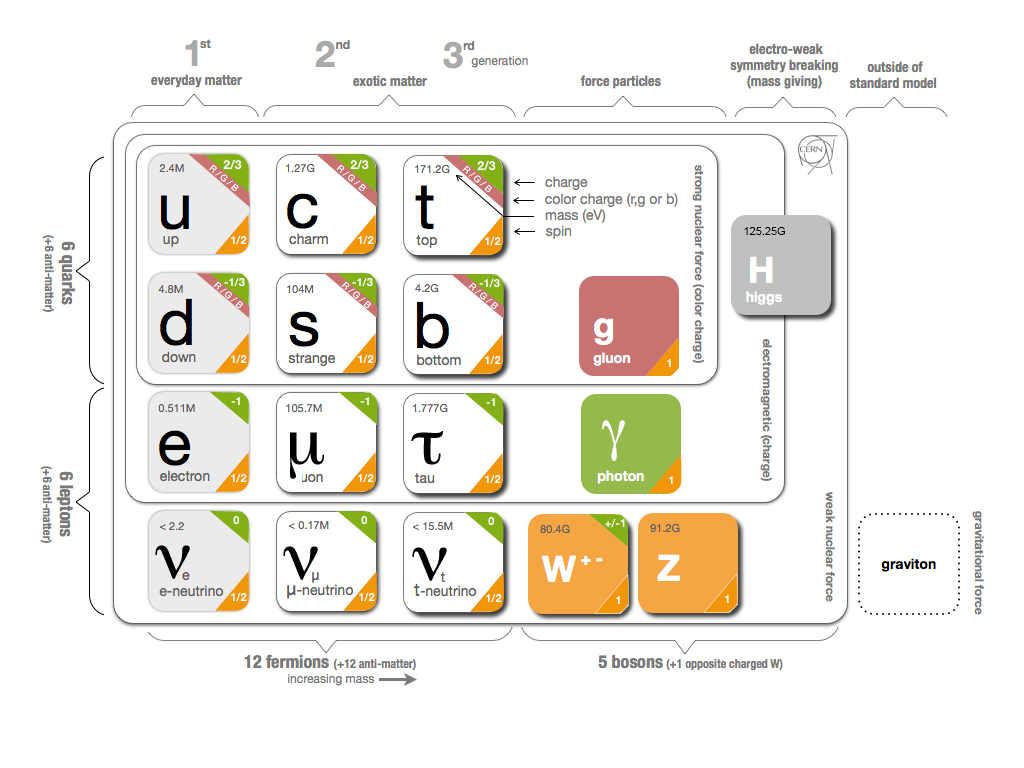
\includegraphics[width=1\textwidth]{SMinfographic_image_}
    \caption[]{Particles in the SM. Adopted from \citep{smpar}. The Higgs Boson mass is corrected to the current value \citep{particle2022review}. }
    \label{fig:sm}
\end{figure}


The fermions can be categorized into three generations each consisting of a charged lepton, a neutral neutrino and two quarks. Except for their masses, particles of different generations have the same quantum numbers. Ordinary matter consists only of particles from the first generation. Moreover each particle has an associated anti-particle with all the quantum numbers inversed.

Quarks possess both electroweak and color charges, causing them to interact with each other via weak, electromagnetic, and strong forces. Each generation consists of an up-type quark (up, charm and top quark) with an electric charge in units of the electron charge of \mbox{Q = + 2/3$e$} and a down-type quark (down, strange and bottom quark) with \mbox{Q = -1/3$e$}. Due to color confinement, quarks can only be observed as composite particles called hadrons, a principle of \ac{qcd} discussed in section \ref{sec:qcd}. Prominent hadrons include mesons (two quarks, e.g., pion) and baryons (three quarks, e.g., proton).

Leptons, which do not carry a color charge, include the electron $e$, muon $\mu$, tau $\tau$, and their associated neutrinos $\nu_e$, $\nu_\mu$, and $\nu_\tau$. Neutrinos have very small masses compared to other particles and are considered massless within the theoretical framework of the \ac{sm}. Neutrinos do not carry an electric charge and interact solely via the weak force, while charged leptons ($e$, $\mu$, $\tau$) with charge $Q=-1$ also interact electromagnetically.

Fermions interact with fields via bosons specific to each force. The strong force is mediated by eight massless gluons $g$, while the electroweak theory includes four massless bosons $W_1,W_2,W_3,B$.

The scalar Higgs particle plays a unique role in the \ac{sm}, breaking the electroweak interaction into weak and electromagnetic interactions through the Higgs mechanism. This process, detailed in section \ref{sec:higgs_mechanism}, explains the observed masses of weak interaction mediators $W^{\pm}$ and $Z$ and also provides an interpretation of the origins of mass for fermions.

If not specified otherwise the following discussions always includes the anti-particles when referred to a species or a particular particle.

\section{Elements of Quantum Field Theory}\label{sec:qft}
Elementary particles can be created, transformed, and annihilated in various forms of particle interactions. These phenomena can be understood through special relativity and quantum mechanics. Special relativity relates energy with mass, allowing energy to manifest as massive particles and vice versa. Quantum mechanics, through the uncertainty principle, states that energy can fluctuate significantly over short time scales.

However, special relativity lacks a quantum mechanical description, and in non-relativistic quantum mechanics, the particle number is conserved. \ac{qft} was developed to provide a solution to this dilemma and to incorporate observations from both fields into a unified theory.

For a field description, some quantity $\phi(x,y,z,t)=\phi(x)$ is assigned to some region in spacetime $x$. Similar to the Lagrangian formalism in classical mechanics, here a Lagrangian density in spacetime governs the dynamics of the system $\mathcal{L}(\phi_1,\dots,\phi_n) =T-V$. Fields which appear in the \ac{sm} and their associated Lagrangians are summarized in table \ref{tab:fields}.
{\renewcommand{\arraystretch}{1.7} %<- modify value to suit your needs
\begin{table}
    \begin{center}
        \begin{tabular}{c|c|c}
            particle           & field type      & Lagrangian                                                                                                   \\ \hline
            spin-0 (scalar)    & scalar $\phi$   & $\mathcal{L}_\mathrm{Klein-Gordon}=\frac{1}{2} (\partial_\mu \phi )(\partial^\mu \phi)-\frac{m^2}{2}\phi^2 $ \\
            spin-1/2 (fermion) & spinor $\psi$   & $\mathcal{L}_\mathrm{Dirac}= \overline{\psi}(i \gamma^\mu \partial_\mu - m )\psi$                            \\
            spin-1 (boson)     & vector  $A_\mu$ & $\mathcal{L}_\mathrm{Proca}= -\frac{1}{4}F_{\mu\nu}F^{\mu\nu} +\frac{m^2}{2} A_\mu A^\mu$                    \\ [.7ex]
        \end{tabular}
        \caption{Quantum fields relevant for the \ac{sm}. With $F_{\mu\nu}=\partial_\mu A_\nu - \partial_\nu A_\mu$ the electromagnetic field strength tensor.}
        \label{tab:fields}
    \end{center}
\end{table}
}
% Via the generalized Euler-Lagrange equations of \ac{qft} 
% \begin{equation}
%     \partial_\mu \left(\frac{\partial\mathcal{L}}{\partial(\partial_\mu\phi_i)}\right)=\frac{\partial\mathcal{L}}{\partial \phi_i}.
% \end{equation}
% the according equations of motion associated with the fields can be obtained.

In \ac{qft} the conventional strategy to describe particle dynamics is to use a perturbation ansatz $\mathcal{L}=\mathcal{L}_0+\mathcal{L}_1$ where one knows the solution of $\mathcal{L}_0$ and adds a small perturbation $\mathcal{L}_1$ so that $\mathcal{L}$ can be solved \citep{zee2010quantum}. Here the free field/kinetic part of the Lagrangian is \mbox{$\mathcal{L}_0=\frac{1}{2}[(\partial_\mu \phi)^2 - m^2\phi^2] $} and a small perturbation/potential term $\mathcal{L}_1=V(\phi)$ is added as some polyominal in $\phi$ that governs the interactions of particles. A term $J(x)\phi(x)$ needs to be added to excite the field or create/destroy particles so that the ansatz reads
\begin{equation}
    \mathcal{L}=\frac{1}{2}[(\partial_\mu \phi)^2 - m^2\phi^2]
    -V(\phi) + J(x)\phi(x).
\end{equation}
In the path integral formulation of \ac{qft} the problem can be reduced to integrals of the form \mbox{$\int D\phi e^{i\int d^4x \mathcal{L}(\phi(\bm{x},t))}$}. Where $\int D\phi$ is the integral over all possible paths of the field. Usually the perturbation $V(\phi)$ is just one anharmonic term with $\lambda\phi^4$ with coupling strength $\lambda$ and is expanded in $e$ to make the integral solvable
\begin{equation}
    e^{-V(\phi)}=e^{-\lambda\phi^4}=1-\lambda\phi^4+\frac{1}{2}\lambda^2\phi^8+\dots
\end{equation}
This only works if $\lambda$ is small. With this the Lagrangian can be solved and the result is a probability also called the amplitude usually denoted with $\mathcal{M}$. Via this one can derive the Feynman rules and calculate cross-sections to a desired order of expansion.

The forces and Lagrangians occurring in the \ac{sm} are discussed in the following sections on \ac{qed} \ref{sec:qed}, \ac{qcd} \ref{sec:qcd} and the \ac{ew} theory \ref{sec:ew}. For these the principle of local gauge invariance plays a key role and is inspired by gauge invariance from classical electrodynamics.

\section{Quantum Electrodynamics}\label{sec:qed}
The \ac{qft}-description of the electromagnetic interaction \ac{qed} can be derived from the free fermion field given by the Dirac equation
\begin{equation}
    \mathcal{L}_\mathrm{Dirac} = \overline{\psi}(i \gamma^\mu \partial_\mu - m )\psi.
    \label{eq:dirac}
\end{equation}
This Lagrangian is invariant, i.e. the equations of motion remain unchanged, under a change of a global phase $\alpha$
\begin{equation}
    \psi(x) \rightarrow  e^{-i \alpha}\psi(x).
\end{equation}
The requirement that this transformation also holds locally means that $\alpha$ now additionally depends on the point $x$ in spacetime $\alpha \rightarrow \alpha(x)$. Since this gives another term because of the derivative, the Lagrangian can be made invariant again by introducing a vector field $A_\mu$ with a coupling of the size of the electron charge $e$ and replacing the derivative $\partial_\mu$ by the covariant derivative $D_\mu$
\begin{equation}
    \partial_\mu \rightarrow D_\mu = \partial_\mu + ie A_\mu.
    \label{eq:cov_diff}
\end{equation}
Thus, the new Lagrangian
\begin{equation}
    \mathcal{L} = \overline{\psi}(i \gamma^\mu D_\mu - m )\psi
    =
    \underbrace{\overline{\psi}(i \gamma^\mu \partial_\mu - m )\psi}_{\mathcal{L}_\mathrm{Dirac} }
    +
    \underbrace{ e\overline{\psi} \gamma^\mu {\psi}A_\mu}_{\mathcal{L}_\mathrm{int}}
\end{equation}
becomes invariant under the local gauge transformations
\begin{align}
    \psi(x)  & \rightarrow  e^{-i \alpha(x)}\psi(x),                      \\
    A_\mu(x) & \xrightarrow{} A_\mu(x) -\frac{1}{e}\partial_\mu\alpha(x),
\end{align}
forming the electromagnetic $U(1)_{EM}$ gauge group.
% The particular scheme of these replacements is also called the minimal substitution rule. 
This Lagrangian describes two fermions interacting with a vector field $A_\mu$ - the photon - represented by the fundamental interaction vertex of \ac{qed} in figure \ref{fig:qed_fundamental}.
\begin{figure}
    \centering
    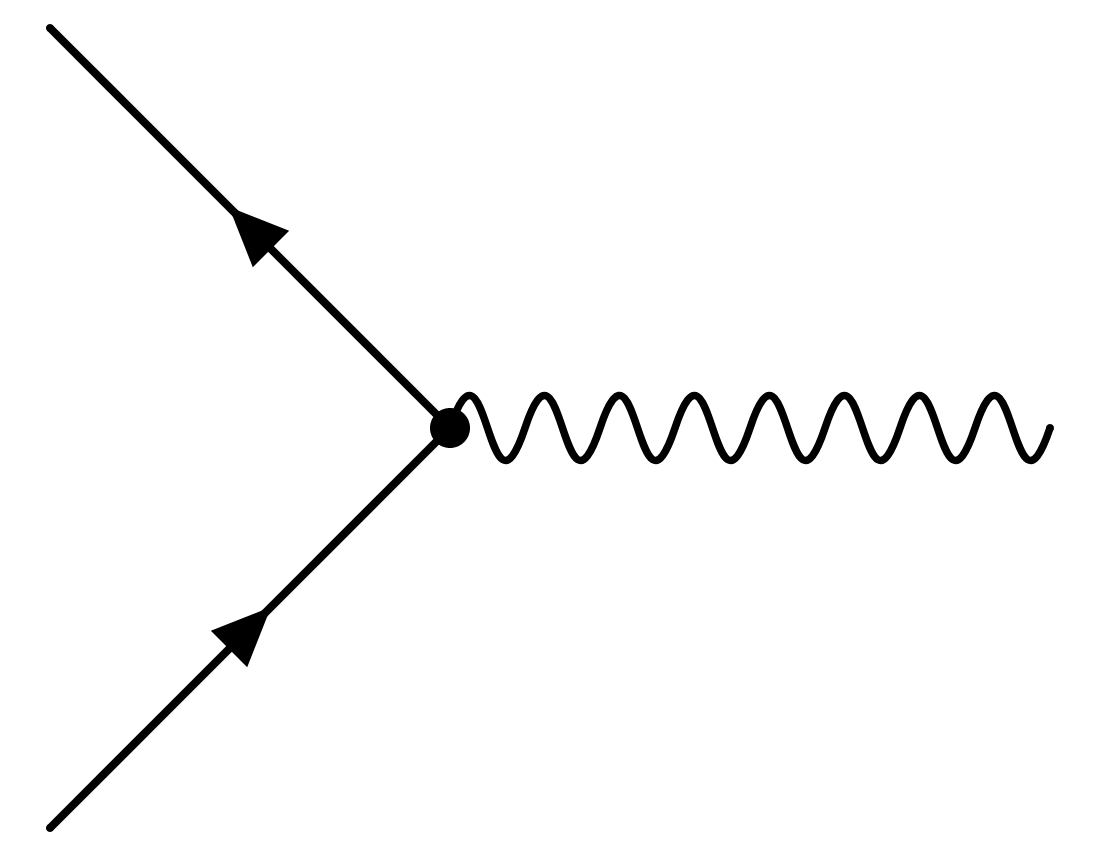
\includegraphics[width=0.27\textwidth]{qed_fundamental}
    \caption[]{The Fundamental interaction vertex of \ac{qed}. Two fermions interacting with a massless photon.}
    \label{fig:qed_fundamental}
\end{figure}
The dyanmics for the photon can be added with the spin-1 Proca Lagrangian from table \ref{tab:fields}. The $F_{\mu\nu}$ term is local gauge invariant whereas $A_\mu A^\mu$ is not, since it picks up a second derivative for $\alpha$ and therefore is required to be massless. The full \ac{qed} lagrangian then reads
\begin{equation}
    \mathcal{L}_\mathrm{QED}
    =
    \underbrace{\overline{\psi}(i \gamma^\mu \partial_\mu - m )\psi}_{\mathcal{L}_\mathrm{Dirac} }
    +
    \underbrace{ e\overline{\psi} \gamma^\mu {\psi}A_\mu}_{\mathcal{L}_\mathrm{int}}
    -
    \underbrace{\frac{1}{4}F_{\mu\nu}F^{\mu\nu}}_{\mathcal{L}_\mathrm{Maxwell} }.
    \label{eq:l_qed}
\end{equation}
That this symmetry holds locally for all unitary $1\times1$ matrices $U(1)$ might seem extravagant, but the formalism is extendable to higher orders as for the \ac{ew} theory and \ac{qcd} case. The gauge group is abelian as any $1\times1$ matrix also commutes with itself. As a result there are no self-interaction terms like $A_\mu A^\mu$ for photons. This means photons only interact with charged particles and not with each other.

\section{Quantum Chromodynamics}\label{sec:qcd}

In a manner similar to how \ac{qed} is derived in section \ref{sec:qed}, the theory of strong interactions, known as \ac{qcd}, is formulated as a non-abelian gauge theory based on the symmetry group $SU(3)$. This group is characterized by the $3\times 3$ Gell-Mann matrices $\lambda_a$ where $a\in\{1,\ldots,8\}$. The fundamental charge in this theory is color, and each quark is represented as a triplet of the three color fermion fields $\Psi_k=(\psi_r,\psi_g,\psi_b)^T$ for all quark flavors $k$. Local gauge invariance of the Lagrangian
\begin{equation}
    \mathcal{L} =
    \sum_k
    \begin{pmatrix}
        \overline{\psi}_r & \overline{\psi}_g & \overline{\psi}_b
    \end{pmatrix}
    (i \gamma^\mu \partial_\mu - m_k )
    \begin{pmatrix}
        \psi_r \\
        \psi_g \\
        \psi_b
    \end{pmatrix}
    =
    \sum_k
    \overline{\Psi}_k(i \gamma^\mu \partial_\mu - m_k )\Psi_k,
    \label{eq:dirac}
\end{equation}
requires the spinors to be invariant under the transformation
\begin{equation}
    \Psi_k(x) \rightarrow e^{i \alpha_a(x) \lambda_a/2} \Psi_k(x),\qquad \alpha\in\mathbb{R},\quad a\in\{1,\mathellipsis,8\},
\end{equation}
with $\alpha_a(x)$ a local phase and the index $a$ for the 8 gluons. It is noted here that summation over equal indices $\alpha_a(x) \lambda_a=\sum_a \alpha_a(x) \lambda_a$ is assumed. As in \ac{qed} a covariant derivative is introduced
\begin{equation}
    D_\mu = \partial_\mu - i g_s \frac{\lambda_a}{2}G_\mu^a,
\end{equation}
involving the eight gluon vector fields $G_\mu^a$ and the coupling strength $g_s$, which is related to the strong coupling constant as
\begin{equation}
    \alpha_s=\frac{g_s^2}{4\pi}.
\end{equation}
With the gluon field strength tensor
\begin{equation}
    G^a_{\mu\nu}=\partial_\mu G_\nu^a-\partial_\nu G_\mu^a+g_s f^a_{\beta\gamma}G^\beta_\mu G_\nu^\gamma, \qquad \text{with } [\lambda_a,\lambda_b]= i f_{ab}^c \lambda_c,
\end{equation}
the gauge invariant \ac{qcd} Lagrangian is
\begin{align}
    {\mathcal {L}}_{\text{QCD}} & =\sum_k\overline{\Psi}_k\left( i \gamma^\mu D_\mu-m_k\right)\Psi_k-{\frac {1}{4}}G_{\mu \nu }^{a}G^{a\mu \nu} \\
                                & =\sum_k
    \underbrace{{\overline{\Psi}_k}\left(i\gamma^\mu \partial_\mu-m_k\right)\Psi_k}_{\mathcal{L}_\text{Kin}}
    \;+ \;
    \underbrace{g_s{\overline{\Psi}_k}\gamma ^{\mu }\frac{ \lambda_a}{2} \Psi_k G_\mu^a}_{\mathcal{L}_\text{Int}}
    \;-\;
    \underbrace{\frac{1}{4}G_{\mu \nu }^{a}G^{a\mu \nu}}_{\mathcal{L}_\text{Self}} .
    \label{eq:l_qcd}
\end{align}
This Lagrangian consists of a kinetic term for each quark, an interaction term of the quarks with the gluons and gluon-gluon interactions resulting in vertices shown in figure \ref{fig:qcd_vertices}. These interactions become apparent when $G^a_{\mu\nu}$ is squared, leading to cubic and quartic terms for the fields.

\begin{figure}[H]
    \centering
    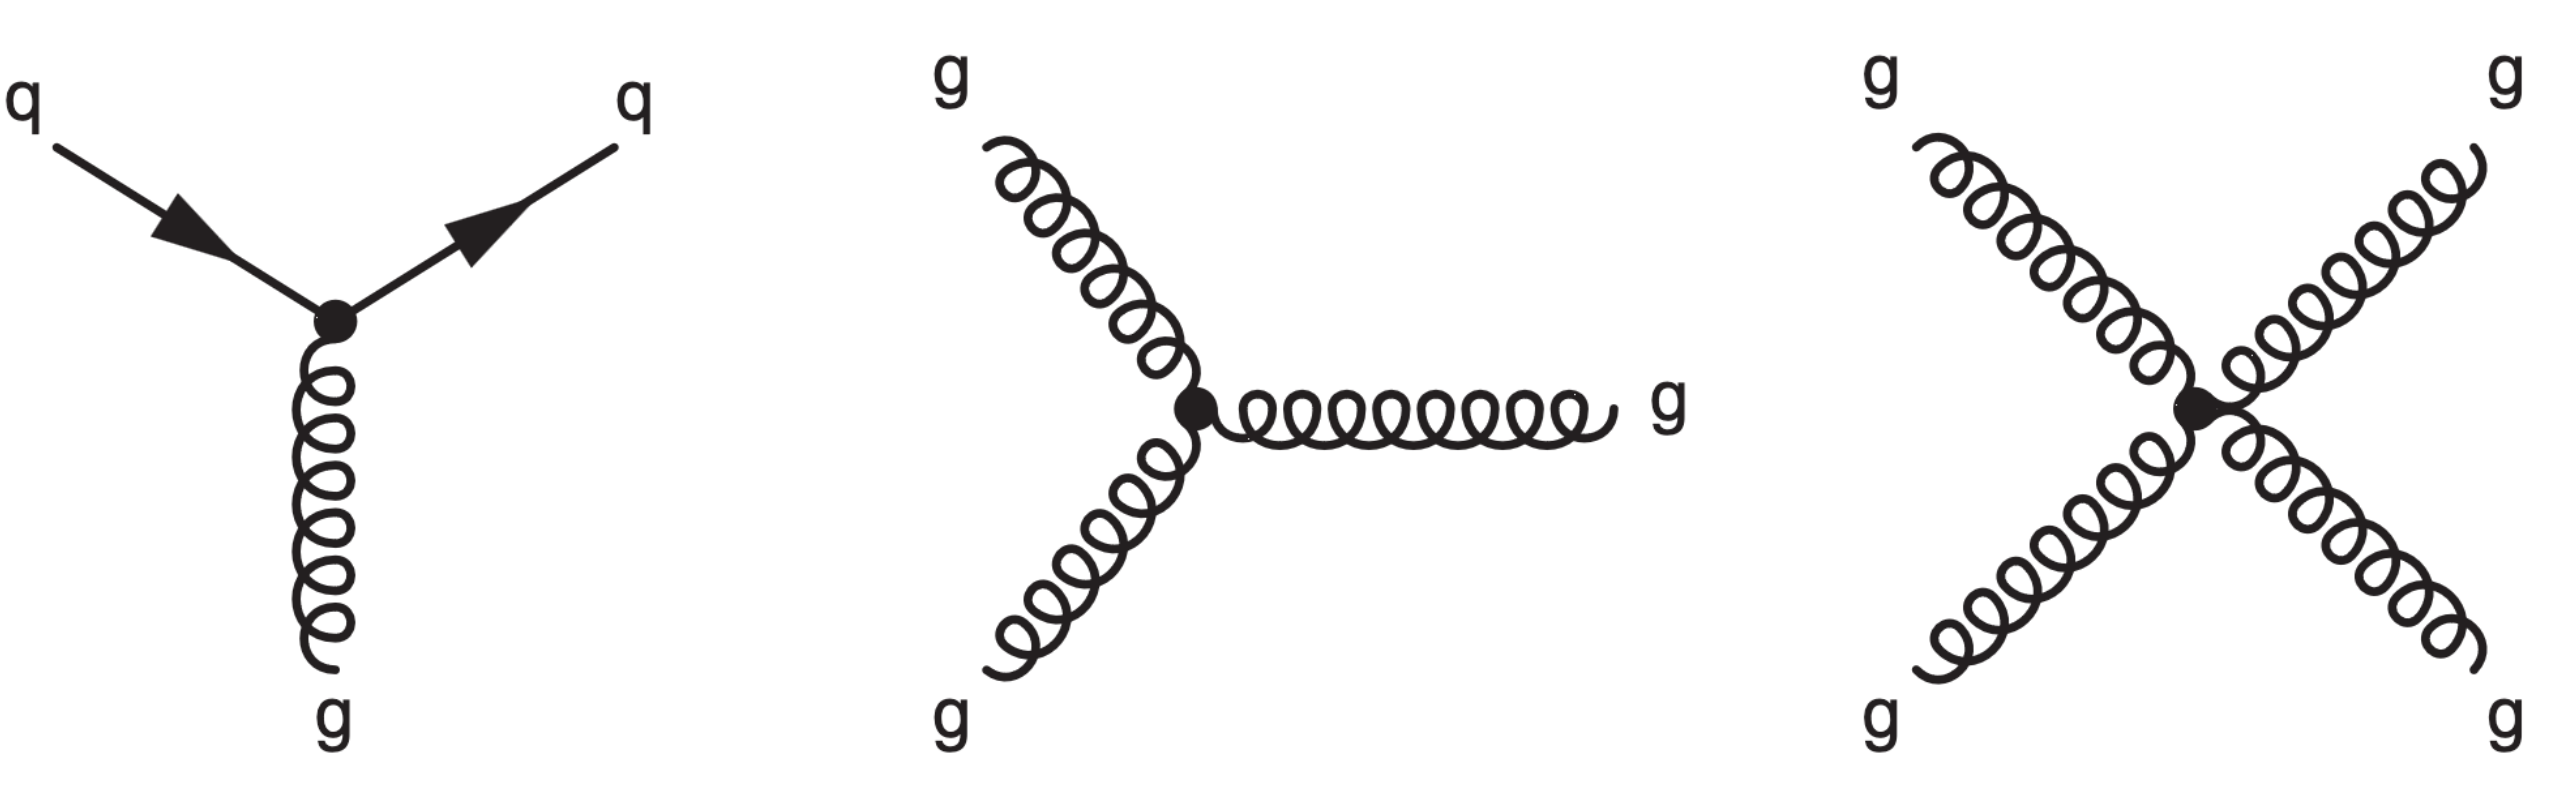
\includegraphics[width=0.8\textwidth]{gluon_gluon_interactions}
    \caption[]{(left) Quarks interacting with a gluon. (middle) triplet and (right) quartic self coupling of gluons. Adopted from \citep{thomson2013modern}.}
    \label{fig:qcd_vertices}
\end{figure}

A unique aspect of \ac{qcd} is color confinement, which states that quarks cannot be observed as free particles; they are always confined within hadrons. This principle arises from the nature of the strong force, which becomes stronger as quarks are pulled apart, a concept further discussed in \ref{sec:renormalization}. Attempts to dissociate hadrons into their quark constituents fails because the formation of quark-antiquark pairs is energetically favoured over separation. This leads to the creation of new hadrons instead of isolated quarks, ensuring that observable particles are always color-neutral.


\section{Electroweak Unification}\label{sec:ew}
The weak force can be incorporated into a gauge-invariant formalism by using a $SU(2)$ symmetry. This is further combined with the electromagnetic force to derive a unified framework for both forces, known as the electroweak interaction, which is described by the symmetry group $SU(2)_L \otimes U(1)_Y$. In this framework, the weak force interacts exclusively with left-handed chiral states of particles, such as for a left-handed fermion $\psi_L$ as expanded on below. Fermions can be grouped by their characteristics into left handed doublets
\begin{equation}
    \begin{pmatrix}
        \nu_e \\ e
    \end{pmatrix}_L, \;
    \begin{pmatrix}
        \nu_\mu \\ \mu
    \end{pmatrix}_L, \;
    \begin{pmatrix}
        \nu_\tau \\ \tau
    \end{pmatrix}_L, \;
    \begin{pmatrix}
        u \\ d
    \end{pmatrix}_L, \;
    \begin{pmatrix}
        c \\ s
    \end{pmatrix}_L, \;
    \begin{pmatrix}
        t \\ b
    \end{pmatrix}_L, \;
    \label{eq:weak_doublets}
\end{equation}
with weak isospin $I=1/2$ that has as third component $I_3=\pm1/2$ for the upper and lower doublet particle respectively. In contrast right handed singlets have $I=0$
\begin{equation}
    e_R    ,\quad \mu_R ,\quad    \tau_R ,\quad    u_R,\quad d_R ,\quad    c_R ,\quad s_R ,\quad    t_R ,\quad b_R.
    \label{eq:weak_singlets}
\end{equation}
The relation between the electric charge of the particle $Q$, $I_3$ and its weak hypercharge $Y$ is governed by the Gell-Mann-Nishijima formula
\begin{equation}
    Q=I_3+Y/2.
    \label{eq:gellmann_nishijima_formula}
\end{equation}
The electroweak Lagrangian is then composed of four basic terms
\begin{equation}
    \mathcal{L}_\mathrm{EW} = \mathcal{L}_\mathrm{fermions}+\mathcal{L}_\mathrm{gauge}+\mathcal{L}_\mathrm{Higgs}+\mathcal{L}_\mathrm{Yukawa}.
    \label{eq:L_EW}
\end{equation}
Following the same steps as for \ac{qcd} and \ac{qed} the Lagrangian can be rendered gauge invariant by introducing a covariant derivative and gauge fields that are dictated by the group symmetry.

$SU(2)$ is generated through the three Pauli matrices $\bm{\sigma}$ requiring three vector gauge fields $W^a_\mu$, $a=\{1,2,3\}$ whereas the $U(1)$ symmetry of the vector gauge field $B_\mu$ is generated by the weak hypercharge $Y$ so the Lagrangian needs to be invariant under the transformation
\begin{align}
    \psi_{L} & \rightarrow e^{i \alpha_a(x) \sigma_a/2}e^{ iY/2} \psi_{L},\qquad & a\in\{1,\mathellipsis,3\} ,\quad \alpha\in\mathbb{R} & \label{eq:gauge_transformation_left}
    \\
    \psi_{R} & \rightarrow e^{ i\beta(x) Y/2} \psi_{R},\qquad                    & \beta\in\mathbb{R}                                   & \label{eq:gauge_transformation_right}
\end{align}
% At this stage the new vector fields are still massless and give the fermionic and gauge parts of the Lagrangian and will be explained below. The masses for the fermions and bosons can be incorporated via the Higgs mechanism that is described in section \ref{sec:higgs_mechanism} yielding the Higgs and Yukawa parts of the Lagrangian.


\subsubsection*{Fermion term}
To distinguish left-handed and right-handed particle states, the corresponding spinors can be written as
\begin{equation}
    \psi_L=\frac{1-\gamma^5}{2}\psi, \quad \psi_R=\frac{1+\gamma^5}{2}\psi,
\end{equation}
where the fifth gamma matrix is defined in terms of the other four gamma matrices as $\gamma^5 = i \gamma^0 \gamma^1 \gamma^2 \gamma^3$. The concept of helicity, which is the projection of a particle's spin along its momentum direction, is useful in understanding these states. However, $\psi_{L}$ and $\psi_{R}$ are not helicity eigenstates but rather select the spinor $\psi$ with the corresponding helicity and vanishes otherwise:
\begin{equation}
    \frac{1}{2}(1 \pm \gamma^5)\psi =
    \begin{cases}
        0    & \text{if } \psi \text{ has helicity } \mp1, \\
        \psi & \text{if } \psi \text{ has helicity } \pm1.
    \end{cases}\label{eq:left_handed_state}
\end{equation}
The aforementioned doublets and singlets are then represented by
\begin{equation}
    \psi_L^j=
    \begin{pmatrix}
        \psi_{L+}^j \\ \psi_{L-}^j
    \end{pmatrix},
    \quad \psi_{R\xi}^k,
\end{equation}
with $j$ running over the doublets from equation \ref{eq:weak_doublets}, $k$ over the singlets from equation \ref{eq:weak_singlets} and $\xi=+$ for u-type fermions and $\xi=-$ for d-type fermions.
The covariant derivative is
\begin{align}
    D_\mu^L & =\partial_\mu- i g_2 \frac{{\sigma}_a}{2}W_\mu^a+i g_1\frac{Y}{2}B_\mu, \label{eq:cov_diff_L} \\
    D_\mu^R & =\partial_\mu+ i g_1\frac{Y}{2}B_\mu,
\end{align}
with coupling $g_2$ and $g_1$ to the vector fields and $\sigma_a$ for the corresponding Pauli matrix, so that the fermionic part of the Lagrangian becomes
\begin{equation}
    \mathcal {L}_\text{fermions} = \sum_j\overline{\psi}^j_L i \gamma^\mu D_\mu^L\psi_L^j+\sum_{j,\xi}\overline{\psi}^j_{R\xi} i \gamma^\mu D_\mu^R\psi_{R\xi}^j.
    \label{eq:L_fermion}
\end{equation}

\subsubsection*{Gauge term}
The gauge field self interaction terms are
\begin{align}
    W_{\mu\nu}^a & =\partial_\mu W_\nu^a-\partial_\nu W_\mu^a+g_2\epsilon_{abc}W_\mu^b W_\nu^c, \\
    B_{\mu\nu}   & =\partial_\mu B_\nu-\partial_\nu B_\mu,
\end{align}
with $g_2$ the weak coupling constant and $\epsilon_{abc}$ the totally asymmetric Levi-Civita tensor yielding the gauge field part of the Lagrangian
\begin{equation}
    \mathcal {L}_\text{gauge} = -\frac{1}{4} W_{\mu\nu}^a W^{\mu\nu,a} - \frac{1}{4}B_{\mu\nu}B^{\mu\nu}.
\end{equation}
So far the \ac{ew} Lagrangian made of the fermions and gauge part describes massless fermions and gauge fields $W^a_\mu$. Up to this point, naive mass terms for the fields listed in table \ref{tab:fields} have been deliberately omitted as they would break gauge invariance. The introduction of masses will be addressed through the Higgs mechanism and Yukawa couplings in the subsequent sections.

% A Proca mass term $\frac{1}{2} m^2 B_\mu B^\mu$ is not invariant as discussed in section \ref{sec:qed}. For a Dirac term like $-m\overline{\psi}\psi$ this can be seen by rewriting it in terms of the left-handed and right-handed fields by inserting a 1 for e.g. the electron and exploiting the transformation of chiral states as of equation \ref{eq:left_handed_state}
% \begin{equation}
%     -m\overline{e}e =
%     -m\overline{e} \left[\frac{1}{2}(1-y^5)+\frac{1}{2}(1+y^5)\right]e
%     =-m(\overline{e}_R e_L+\overline{e}_L e_R).
%     \label{eq:yukawa_mass_term}
% \end{equation}
% $\overline{e}_R$ is a $SU(2)$ singlet and $e_L$ is one component of a $SU(2)$ doublet and therefore such a term is not gauge invariant. 


\section{Higgs Mechanism}\label{sec:higgs_mechanism}

% \red{
%     The scalar Higgs particle has a unique role in the Standard model. A locally gauge invariant \ac{qft} requires massless mediators, which the $W^{\pm},Z$ are not. When unifying the weak force and the electromagnetic force into the electroweak force a new field - the Higgs field - incorporates mass to these mediators by leaving the \ac{qft} gauge invariant. This will be discussed in detail in section \ref{sec:higgs_mechanism}. The Higgs field can also explain the masses of all fermions as the coupling to each fermion is proportional to its mass. This essentially means that the heavier the particle, the stronger its interaction is with the Higgs field.
% }
In the previous sections it was shown that the principle of local gauge invariance applied to the free Dirac Lagrangian can generate all the dynamics for a given interaction. However, this assumes that the accompanying gauge boson vector fields are massless, which is not the case for the weak interactions. The Higgs mechanism adds a field to the Lagrangian that provides mass terms for the vector bosons and fermions while preserving the principle of local gauge invariance. A way to implement this for a $U(1)$ symmetry is to consider two scalar fields $\phi_1$ and $\phi_2$ and combine them into a complex scalar field
\begin{equation}
    \phi (x)=\frac{1}{\sqrt{2}}(\phi_1(x)+i\phi_2(x)).
\end{equation}
A Lagrangian with a kinetic term $T(\phi)$ and a potential $V(\phi)$ with parameters $\mu$ and $\lambda$ can then be written as
\begin{equation}
    \mathcal{L}=T(\phi)-V(\phi)=
    \left[\left(\partial_\mu\phi\right)^* (\partial^\mu\phi)\right]
    -\left[
        -\mu^2(\phi^*\phi)+\lambda(\phi^*\phi)^2
        \right].
\end{equation}
This Lagrangian can be made local gauge invariant under a $U(1)$ symmetry by following the transformation steps used in \ac{qed} from section \ref{sec:qed} by replacing the derivative with the covariant derivative with some vector field $B_\mu$ and coupling $g$
\begin{equation}
    \partial_\mu \rightarrow D_\mu = \partial_\mu + ig B_\mu.
\end{equation}
The transformations for the scalar and gauge fields are given as
\begin{align}
    \phi(x)  & \rightarrow  e^{i g\alpha(x)}\phi(x), \label{eq:scalar_local_gauge} \\
    B_\mu(x) & \xrightarrow{} B_\mu(x) -\partial_\mu\alpha(x).
\end{align}
The lowest energy state of a \ac{qft} is the vacuum state and therefore its eigenvalue is also called \ac{vev}. Here it is the one that minimizes the potential $V(\phi)$
\begin{equation}
    v =
    \begin{cases}
        0                                                     & \lambda>0, \mu^2<0  \\
        \sqrt{\phi_1^2+\phi_2^2}=\sqrt{\frac{\mu^2}{\lambda}} & \lambda>0, \mu^2>0,
    \end{cases}
\end{equation}
and is either 0 or forms an infinite set of minima as illustrated in figure \ref{fig:higgs_potential} by the dashed circle.
\begin{figure}
    \centering
    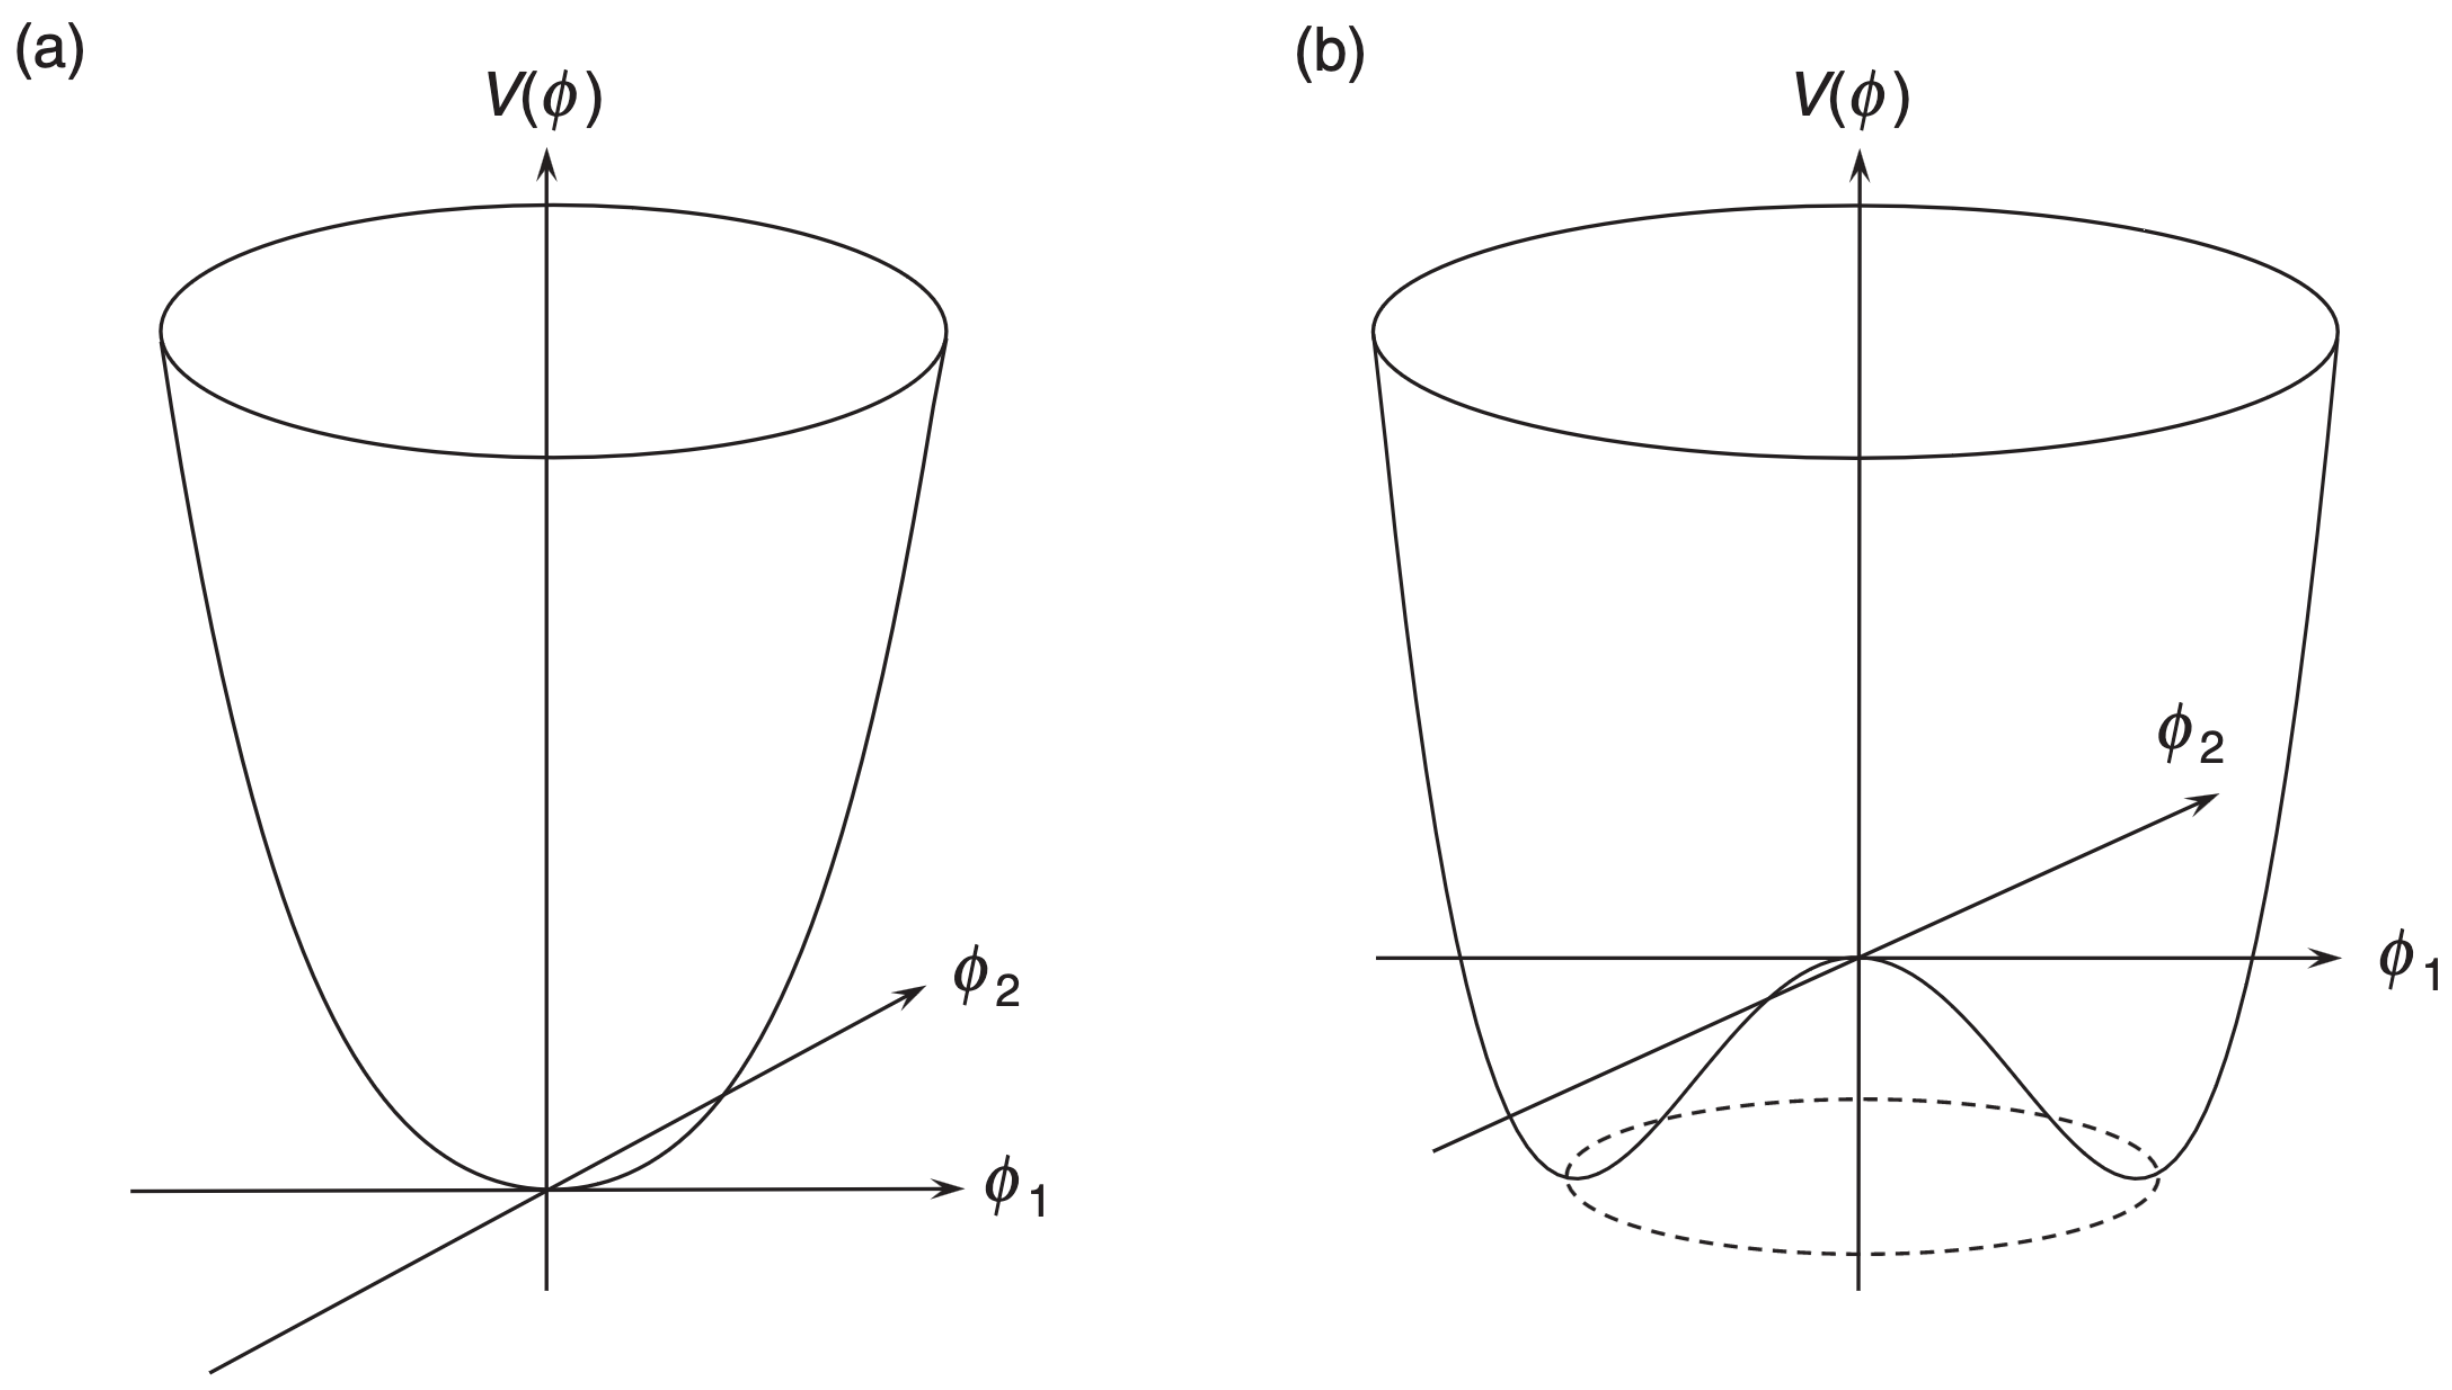
\includegraphics[width=.8\textwidth]{higgs_potential}
    \caption[]{Potential $V(\phi)$: (\textbf{a}) for $\lambda>0$ and $\mu^2<0$ and (\textbf{b}) for values $\lambda>0$ and $\mu^2>0$. Adopted from \citep{thomson2013modern}.}
    \label{fig:higgs_potential}
\end{figure}

The \ac{qft} perturbation ansatz from section \ref{sec:qft} starts from perturbations around the ground state. Thus for the ansatz to work with the $\mu^2>0$ case new field variables $\eta(x)$ and $\xi(x)$ can be introduced so the perturbation calculus can be applied about the ground state
\begin{equation}
    \phi_1(x)=v+\eta(x),\quad \phi_2(x)=\xi(x).
\end{equation}
The physical vacuum state spontaneously breaks the symmetry of the Lagrangian. Furthermore the physical predictions of the Lagrangian do not depend on the choice of the gauge and can be chosen in a way that it eliminates the field $\xi (x)$. In particular, if $\alpha(x)=-\xi(x)/(gv)$, the transformation from equation \ref{eq:scalar_local_gauge} can be made unitary ($UU^\dagger=1$) when expressed to first order in the field variables. Moreover $\eta(x)$ can then be reinterpreted as a Higgs field $h(x)$
\begin{equation}
    \phi(x)  \rightarrow  e^{i g\alpha(x)}\frac{1}{\sqrt{2}}(v+\eta(x)+i\xi(x))
    \approx
    \frac{1}{\sqrt{2}}e^{-i \frac{\xi(x)}{v}}[v+\eta(x)]e^{i\frac{\xi(x)}{v}}
    =
    \frac{1}{\sqrt{2}}(v+h(x)).
\end{equation}
The full local gauge invariant Lagrangian for a $U(1)$ complex scalar field then reads except for constants
\begin{align}
    \mathcal{L}= &
    \underbrace{\frac{1}{2}(\partial_\mu h)(\partial^\mu h)-\lambda v^2 h^2}_{\text{massive h scalar}}
    -
    \underbrace{\frac{1}{4}F_{\mu\nu}F^{\mu\nu} -\frac{1}{2}g^2v^2 B_\mu B^\mu}_{\text{massive boson}}
    \nonumber
    \\
                 & + \underbrace{g^2vB_\mu B^\mu h+\frac{1}{2}g^2 B_\mu B^\mu h^2}_{\text{h,B interactions}}
    -
    \underbrace{\lambda v h^3 -\frac{1}{4}\lambda h^4}_{\text{h self-interactions}},
\end{align}
and describes a massive scalar particle $h$, a massive boson $B_\mu$, interactions between the scalar and boson and as well interactions of the scalar itself depicted in figure \ref{fig:higgs_couplings}.
\begin{figure}
    \centering
    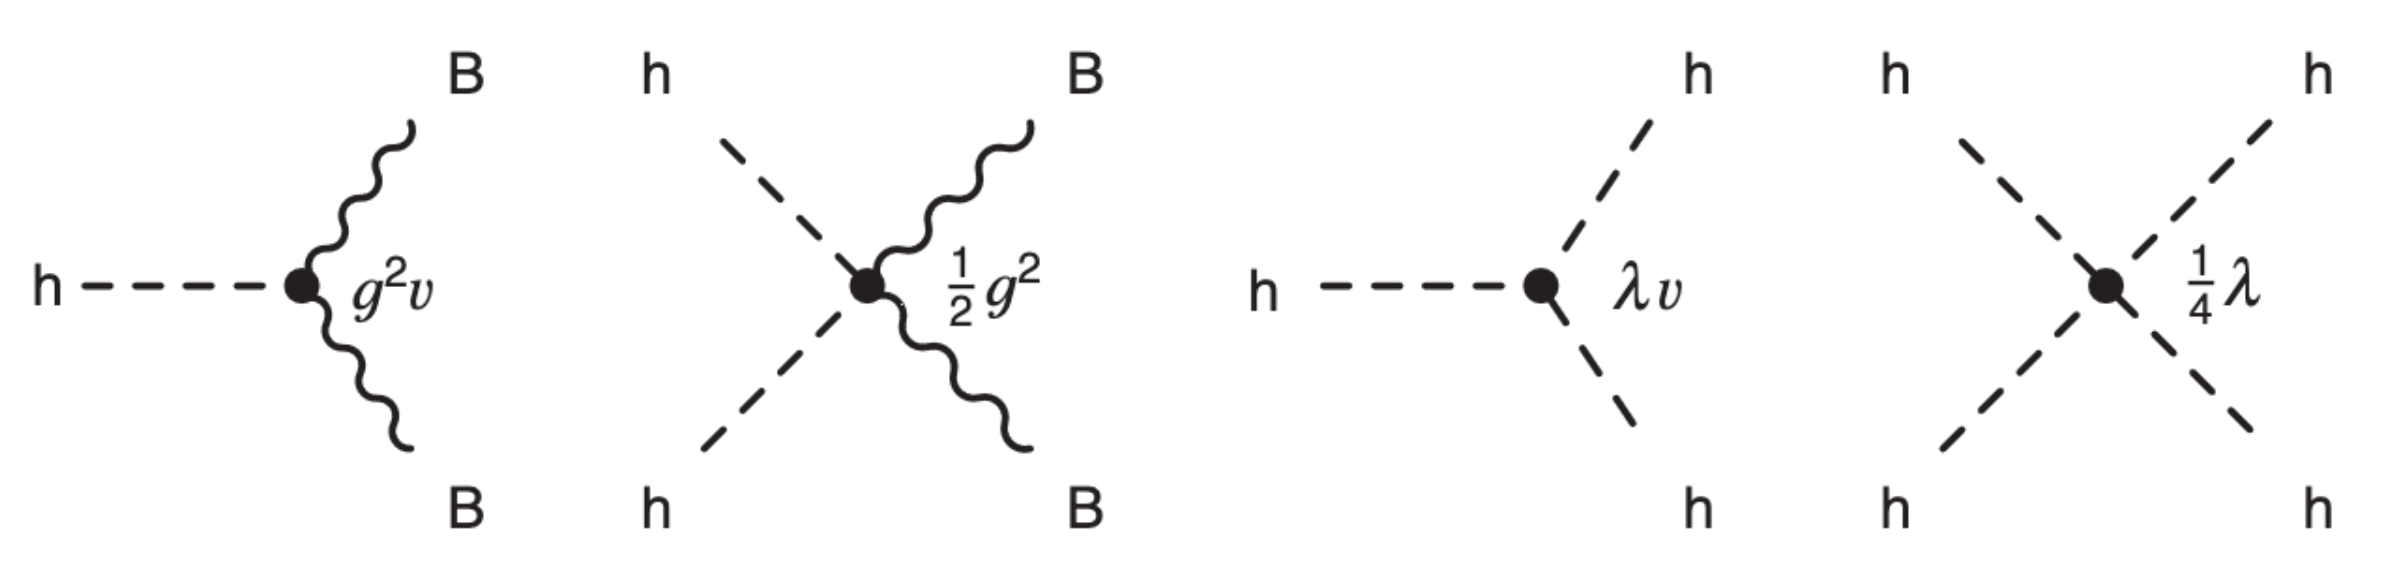
\includegraphics[width=.8\textwidth]{higgs_couplings}
    \caption[]{Self-interactions of a Higgs from a local $U(1)$ gauge symmetry. Adopted from \citep{thomson2013modern}.}
    \label{fig:higgs_couplings}
\end{figure}

\subsection*{The Standard Model Higgs}
For the electroweak Lagrangian the $SU(2)_L \otimes U(1)_Y$ symmetry is broken by the Higgs mechanism while maintaining the electromagnetic $U(1)_{EM}$ symmetry. This is also called \ac{ewsb} and is realized with a isospin doublet of complex scalar fields
\begin{equation}
    \phi(x)=
    \begin{pmatrix}
        \phi^+(x) \\
        \phi^0(x)
    \end{pmatrix}
    =
    \begin{pmatrix}
        \phi_1 (x)+i \phi_2 (x) \\
        \phi_3 (x)+i \phi_4 (x)
    \end{pmatrix}.
\end{equation}
with weak hyperchage $Y=1$. The upper state $\phi^+$ with $I_3=1/2$ is electrically charged and the lower state $\phi^0$ with $I_3=-1/2$ is electrically neutral consistent with the Gell-Mann Nishijima formula from equation \ref{eq:gellmann_nishijima_formula}.


\subsubsection*{Higgs Term}
With $Y=1$ the covariant derivative from equation \ref{eq:cov_diff_L} becomes
\begin{equation}
    D_\mu=\partial_\mu- i g_2\frac{{\sigma}_a}{2}W_\mu^a+ ig_1\frac{1}{2}B_\mu.
\end{equation}
and the Higgs term for the electroweak Lagrangian of equation \ref{eq:L_EW} is
\begin{equation}
    \mathcal{L}_\text{Higgs}= \left(D_\mu\phi\right)^\dagger (D^\mu\phi)-V(\phi),
    \label{eq:L_higgs}
\end{equation}
with the Higgs potential
\begin{equation}
    V(\phi) = -\mu^2\phi^\dagger\phi+\frac{\lambda}{4}\left(\phi^\dagger\phi\right)^2.
    \label{eq:Higgs_initial_potential}
\end{equation}
In analogy to the steps for the $U(1)$ Higgs mechanism from section \ref{sec:higgs_mechanism} there is a set of degenerate minima for $\mu^2,\lambda>0$
\begin{equation}
    \phi^\dagger\phi=\frac{1}{2}(\phi_1^2+\phi_2^2+\phi_3^2+\phi_4^2)=\frac{v^2}{2}=\frac{4\mu^2}{\lambda}.
    \label{eq:higgs_vev}
\end{equation}
Since the photon needs to remain massless and as shown in section \ref{sec:higgs_mechanism} broken symmetries generate gauge bosons with mass, the \ac{vev} is chosen in a way that the vacuum shares the symmetry of the electromagnetic gauge group $U(1)_{EM}$ from section \ref{sec:qed} via setting \mbox{$\phi_1=\phi_2=\phi_4=0$} and $\phi_3=v$ such that the \ac{vev} becomes
\begin{equation}
    \langle0\vert \phi \vert0\rangle=\phi_0=\frac{1}{\sqrt{2}}
    \begin{pmatrix}
        0 \\
        v
    \end{pmatrix}.
\end{equation}
The generator of the electromagnetic subgroup is $Q=I_3+Y/2$. $\phi_0$ breaks $SU(2)_L$ and $U(1)_Y$ but since the lower state is electrically neutral $Q=0$, it remains local gauge invariant under $U(1)_{EM}$ as can be seen from
\begin{equation}
    \phi_0 \rightarrow e^{i\alpha(x)Q}\phi_0=\phi_0.
\end{equation}
Expanding the field about the \ac{vev}
\begin{equation}
    \phi(x)=\frac{1}{\sqrt{2}}
    \begin{pmatrix}
        \phi_1 (x)+i \phi_2 (x) \\
        v+ \eta(x)+i \phi_4 (x)
    \end{pmatrix},
\end{equation}
becomes in the unitary gauge with the physical \ac{sm} Higgs field $h$
\begin{equation}
    \phi(x)=\frac{1}{\sqrt{2}}
    \begin{pmatrix}
        0 \\
        v+h(x)
    \end{pmatrix}.
    \label{eq:unitary_gauge}
\end{equation}
In this form the potential then becomes with equation \ref{eq:higgs_vev} in terms of $\mu$ and $v$
\begin{equation}
    V=\mu^2h^2+\frac{\mu^2}{v}h^3+\frac{\mu^2}{4v^2}h^4
    =
    \frac{m_h^2}{2}h^2+\frac{m_h^2}{2v}h^3+\frac{m_h^2}{8v^2}h^4.
    \label{eq:higgs_potential}
\end{equation}
This yields a Higgs mass term $m_h=\mu\sqrt{2}$ and triplet and quartic self-couplings proportional to the Higgs mass. The kinematic term of the Higgs Lagrangian can be brought into a form that the gauge fields $W^1_\mu,W^2_\mu,W^3_\mu,B_\mu$ represent the physical fields: the charged massive $W^{\pm}$ gauge bosons then are
\begin{equation}
    W_\mu^\pm = \frac{1}{\sqrt{2}}(W_\mu^1\mp i W_\mu^2),
\end{equation}
and the neutral massive $Z$ boson and the massless photon $A_\mu$ are mixed states of
\begin{equation}
    \begin{pmatrix}
        A_\mu \\
        Z_\mu
    \end{pmatrix}
    =
    \begin{pmatrix}
        \cos\theta_W  & \sin\theta_W \\
        -\sin\theta_W & \cos\theta_W
    \end{pmatrix}
    \begin{pmatrix}
        B_\mu \\
        W^3_\mu
    \end{pmatrix}
\end{equation}
rotated by the Weinberg weak mixing angle $\theta_W$. The kinematic Higgs term then becomes
\begin{equation}
    \left(D_\mu\phi\right)^\dagger (D^\mu\phi )=
    \frac{1}{2}(\partial_\mu h)(\partial^\mu h)+
    \frac{g_2^2}{4}W^-_\mu W^{+\mu}(v+h)^2+
    \frac{g_1^2+g_2^2}{4} Z_\mu Z^\mu(v+h)^2.
    \label{eq:higgs_kinematic}
\end{equation}
% \begin{align}
%     \left(D_\mu\phi\right)^\dagger (D^\mu\phi )= &
%     \frac{1}{2}(\partial^\mu h)(\partial_\mu h)+
%     \frac{g_2^2}{4}W^-_\mu W^{+\mu}(v+h)^2+
%     \\
%                                                  & \frac{1}{2}\begin{pmatrix}
%                                                                   A_\mu & Z_\mu
%                                                               \end{pmatrix}
%     \begin{pmatrix}
%         m_A^2 & 0     \\
%         0     & m_Z^2
%     \end{pmatrix}
%     \begin{pmatrix}
%         A_\mu \\
%         Z_\mu
%     \end{pmatrix}
% \end{align}
and describes trilinear $HWW,HZZ$ and quadrilinear $HHWW,HHZZ$ vertices. The photon becomes naturally massless in this form and the masses of the massive gauge bosons can be read off
\begin{equation}
    m_W= \frac{1}{2}g_2v,\quad m_Z=\frac{1}{2}\sqrt{g_1^2+g_2^2}.
\end{equation}
Furthermore a relation to the weak mixing angle and the electric charge follow
\begin{equation}
    \cos\theta_W=\frac{g_2}{\sqrt{g_1^2+g_2^2}}=\frac{m_W}{m_Z}, \quad e=g\sin \theta_W.
\end{equation}
The $\cos\theta_W$ was experimentally verifiable before the Higgs discovery and a compelling argument for the Higgs to exist.



\subsubsection*{Yukawa Term}\label{sec:yukawa_term}
Fermion masses can be incorporated into the electroweak Lagrangian of equation \ref{eq:L_EW} with the help of the Higgs mechanism in the form of Yukawa couplings. For one generation of leptons and quarks gauge invariant terms are introduced via couplings between the left-handed doublet states, the Higgs field and right handed singlet states
\begin{align}
    \mathcal{L}_\mathrm{Y}^{\text{one gen}} & =
    - \; G_e
    \begin{pmatrix}
        \overline{\nu}_e & \overline{e} \\
    \end{pmatrix}_L
    \begin{pmatrix}
        \phi^+ \\
        \phi^0
    \end{pmatrix}
    e_R                                                                                                                                                                \\
                                            & \phantom{-\;}-G_d
    \begin{pmatrix}
        \overline{u} & \overline{d} \\
    \end{pmatrix}_L
    \begin{pmatrix}
        \phi^+ \\
        \phi^0
    \end{pmatrix}
    d_R                                                                                                                                                                \\
                                            & \phantom{-\;}-G_u
    \begin{pmatrix}
        \overline{u} & \overline{d} \\
    \end{pmatrix}_L
    \begin{pmatrix}
        \phi^{0*} \\
        -\phi^-
    \end{pmatrix}
    u_R                                                                                                                                                                \\
                                            & \phantom{-\;} +h.c.                                                                                                      \\
                                            & = -G_e \overline{L}_L \phi e_R -G_d \overline{Q}_L \phi d_R -G_u \overline{Q}_L \phi_c e_R + h.c. \label{eq:L_Y_one_gen}
\end{align}
with Yukawa coupling constant $G_e,G_d,G_u$ and the charge conjugated Higgs field $\phi_c=i\sigma_2\phi$. The latter can be used because it transforms just like the Higgs field and therefore leaves the Lagrangian gauge invariant. In the unitary gauge mass terms arise e.g. for the electron in the form
\begin{equation}
    \mathcal{L}_\mathrm{Y}^e=\frac{-G_e}{\sqrt{2}} v (\overline{e}_L e_R+\overline{e}_R e_L)+\frac{-G_e}{\sqrt{2}} h (\overline{e}_L e_R+\overline{e}_R e_L).
\end{equation}
The mass of a fermion $f$ is therefore
\begin{equation}
    m_f=G_f\frac{v}{\sqrt{2}},
\end{equation}
so that the full Yukawa Lagrangian can be written as
\begin{equation}
    \mathcal{L}_\mathrm{Yukawa}=-\sum_f m_f\overline{\psi}_f \psi_f -\sum_f \frac{m_f}{v}\overline{\psi}_f \psi_f h.
    \label{eq:yukawa_term}
\end{equation}
Consequently the Higgs couples to fermions proportional to their masses. Since physically observed states are mixed states of the $\psi_f$ eigenstates for the charged weak interactions, the formalism can be extended by making the Yukawa couplings $3\times 3$ matrices $G_u=G_{ij}^d$ with $i=u,c,t$ going over up type quarks and $j=d,s,b$ over down type quarks. Thus the quark part of the Yukawa Lagrangian of equation \ref{eq:L_Y_one_gen} becomes
\begin{equation}
    \mathcal{L}_\mathrm{Y}^{\text{quarks}} =
    -G_{ij}^d \overline{Q}_L^i \phi d_R^j -G_{ij}^u \overline{Q}_L^i \phi_c e_R^j + h.c.
\end{equation}
The $G_{ij}$ matrices mix the eigenstates and can be diagonalized with four unitary matrices $V_{L,R}^{u,d}$
\begin{equation}
    \Tilde{u}^i_{L,R}=(V^u_{L,R})_{ik}u^k_{L,R}, \quad \Tilde{d}^i_{L,R}=(V^d_{L,R})_{ik}u^k_{L,R}.
\end{equation}
With the identity $V_L^uV_L^{d\dagger}\equiv V_\mathrm{CKM}$ the quark mixing matrix also called \acf{ckm} matrix mixes the physical quark eigenstates
\begin{equation}
    \begin{pmatrix}
        d' \\
        s' \\
        b' \\
    \end{pmatrix}
    =V_\mathrm{CKM}\begin{pmatrix}
        d \\
        s \\
        b \\
    \end{pmatrix}=
    \begin{pmatrix}
        V_{ud} & V_{us} & V_{ub} \\
        V_{cd} & V_{cs} & V_{cb} \\
        V_{td} & V_{ts} & V_{tb} \\
    \end{pmatrix}
    \begin{pmatrix}
        d \\
        s \\
        b \\
    \end{pmatrix}.
\end{equation}
The $V_{ij}$ describes the transition probability for a quark $j$ to quark $i$ via the charged weak interactions. In this model neutrinos are assumed to be massless. While it is theoretically possible to incorporate neutrino masses into the \ac{sm}, the mechanism for doing so remains unclear. Introducing neutrino mass terms in a manner similar to that of up-type quarks requires to introduce right-handed neutrinos, which have not been observed. This completes the current \ac{sm} electroweak Lagrangian of equation \ref{eq:L_EW}.

\section{Renormalization}\label{sec:renormalization}
\begin{figure}
    \centering
    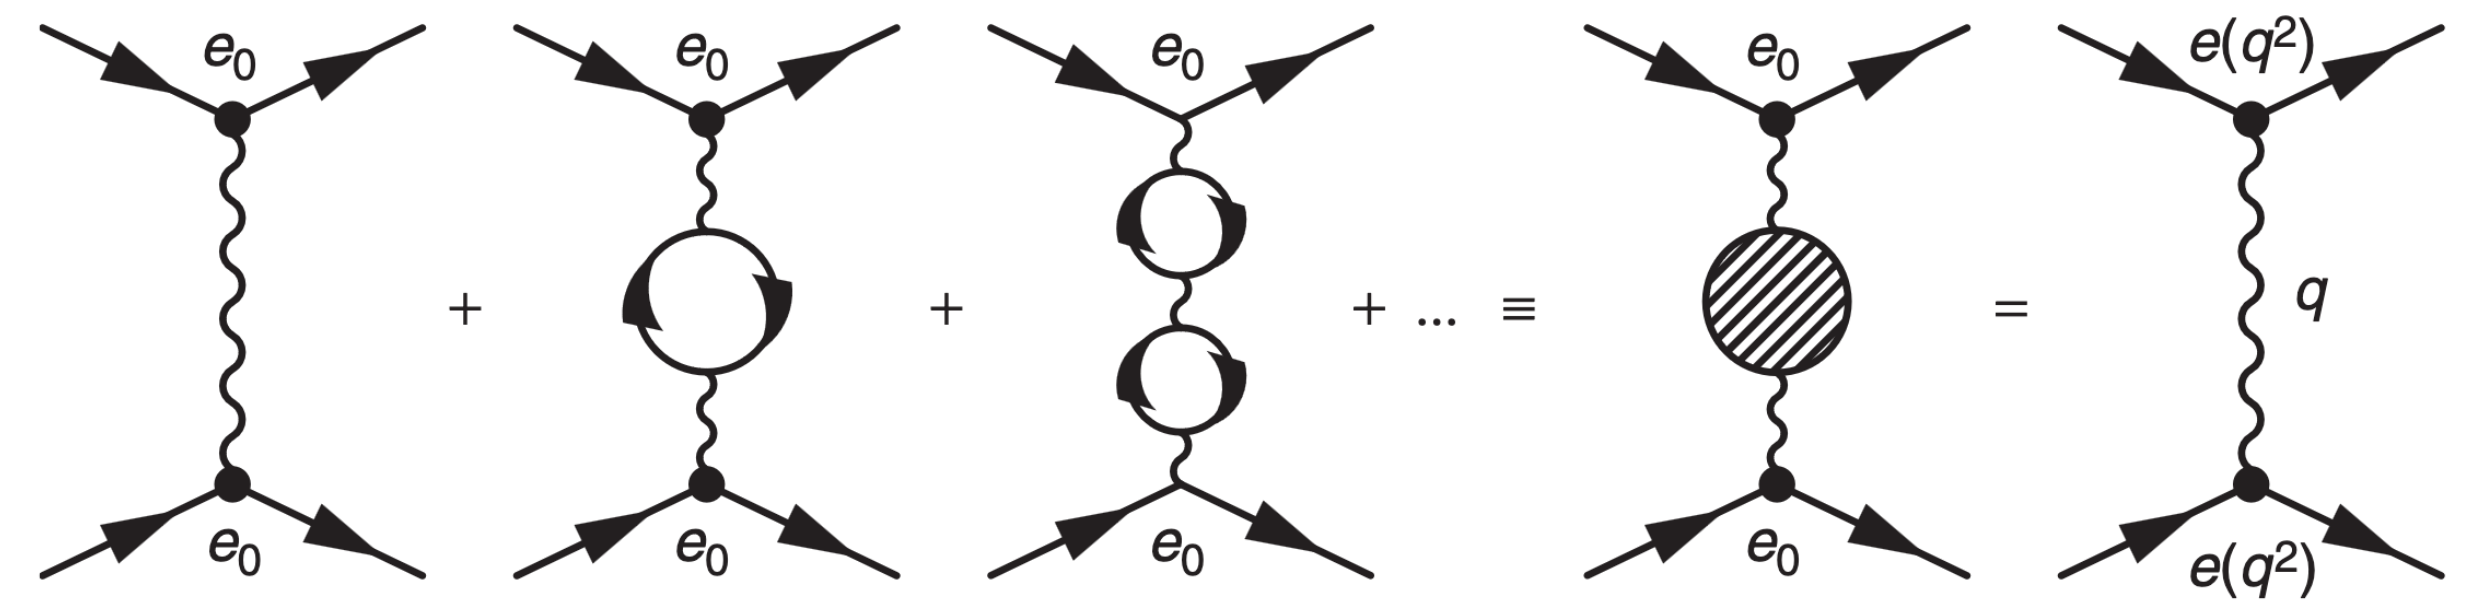
\includegraphics[width=1\textwidth]{qed_diagrams}
    \caption[]{Higher order loop corrections in \ac{qed} schematically treated as one effective diagram. Adopted from \citep{thomson2013modern}.}
    \label{fig:qed_diagrams}
\end{figure}
When attempting to calculate amplitudes $\mathcal{M}$ for higher-order diagrams in \ac{qed}, such as the second or third diagrams shown in Figure \ref{fig:qed_diagrams}, it results in diverging integrals. This phenomenon, known as vacuum polarization, occurs as virtual particle-antiparticle pairs act to screen the actual charge of the electron $e_0$, analogous to a dielectric medium in classical electrodynamics. To address this issue, an effective charge/coupling $e(q^2)$ is introduced. This coupling becomes a function of the squared four-momentum $q^2$ at the virtual photon vertex, as depicted in Figure \ref{fig:qed_diagrams} and renders the integrals finite.

For the second diagram in figure \ref{fig:qed_diagrams} with only one loop correction, it can be shown that for some measured coupling $e(q^2=\mu^2)$ at an energy scale $\mu^2$, the actual coupling $e(q^2)$ follows a scaling behavior that holds if $q^2$ and $\mu^2$ are larger than the electron mass \citep{thomson2013modern}. The coupling constant is now a running coupling $e(q^2)$ and reads in terms of the fine structure constant $\alpha(q^2)=e^2(q^2)/4\pi$,
\begin{equation}
    \alpha(q^2)=
    \frac{\alpha(\mu^2)}
    {1-\alpha(\mu)\frac{1}{3\pi}
        \ln
        \left(\frac{q^2}{\mu^2}\right)}.
    \label{eq:qed_coupling}
\end{equation}
Therefore with increasing momentum transfer, or a decreasing distance when colliding particles, the number of virtual pair production processes is effectively reduced, revealing the bare charge of the electron. This behavior is shown qualitatively in figure \ref{fig:renorm_scaling}(a).
\begin{figure}
    \centering
    \subfigure[]{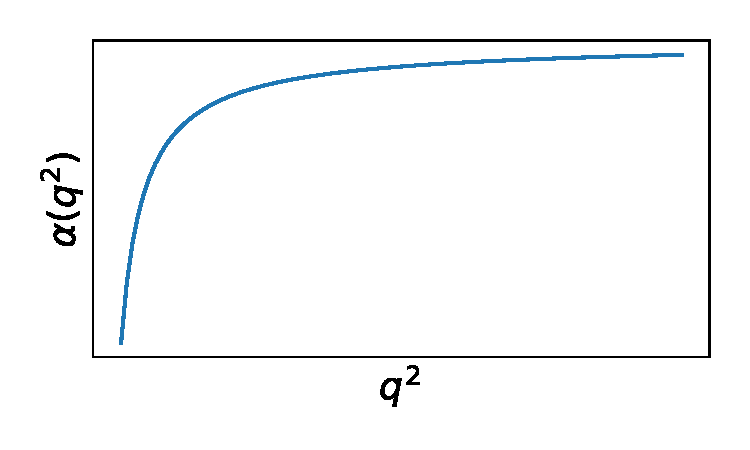
\includegraphics[width=.49\textwidth]{qed_scaling}}
    \subfigure[]{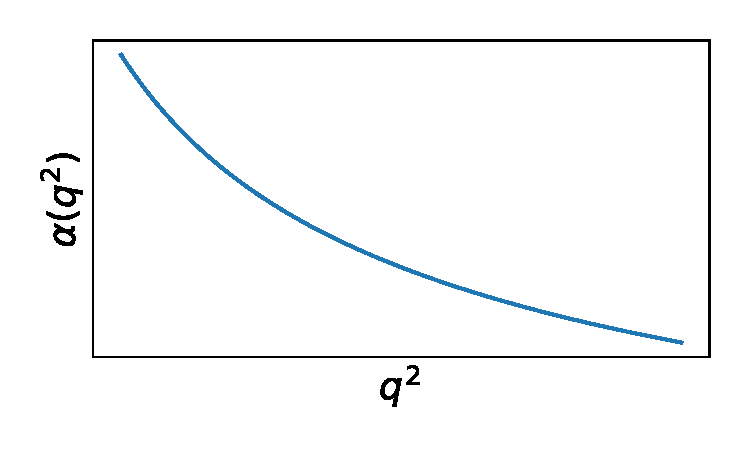
\includegraphics[width=.49\textwidth]{qcd_scaling}}
    \caption[]{Qualitative behavior of the running couplings for (\textbf{a}) \ac{qed} as of equation \ref{eq:qed_coupling} and (\textbf{b}) \ac{qcd} as of equation \ref{eq:qcd_coupling}.}
    \label{fig:renorm_scaling}
\end{figure}
\begin{figure}[H]
    \centering
    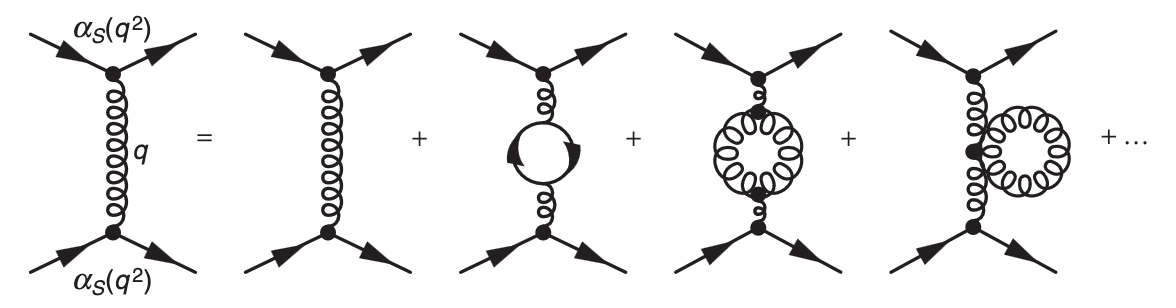
\includegraphics[width=1\textwidth]{qcd_diagrams}
    \caption[]{Some higher order loop corrections in \ac{qcd}. Adopted from \citep{thomson2013modern}.}
    \label{fig:qcd_diagrams}
\end{figure}
Renormalization in \ac{qcd} can be derived similarly but also the quartic and triplet couplings exemplified in figure \ref{fig:qcd_diagrams} need to be considered. This results in a scaling for the strong coupling
\begin{equation}
    \alpha_S(q^2)=
    \frac{\alpha_S(\mu^2)}
    {1+B\alpha_S(\mu)
        \ln
        \left(\frac{q^2}{\mu^2}\right)}, \qquad \text{with } B=\frac{11N_c-2N_f}{12\pi}.
    \label{eq:qcd_coupling}
\end{equation}
For 3 color charges $N_c$ and 6 flavors $N_f$ in the \ac{sm}, $B$ is positive and the coupling becomes weaker for shorter scales or higher momentum transfer as can be seen in figure \ref{fig:renorm_scaling}(b).

The fine structure constant of \ac{qed} $\alpha(q^2\approx 0)\approx 1/137$ does not vary dramatically over the energy ranges of matter for particle physics as shown in figure \ref{fig:renorm_scaling_exp}(a).
\begin{figure}
    \centering
    \subfigure[]{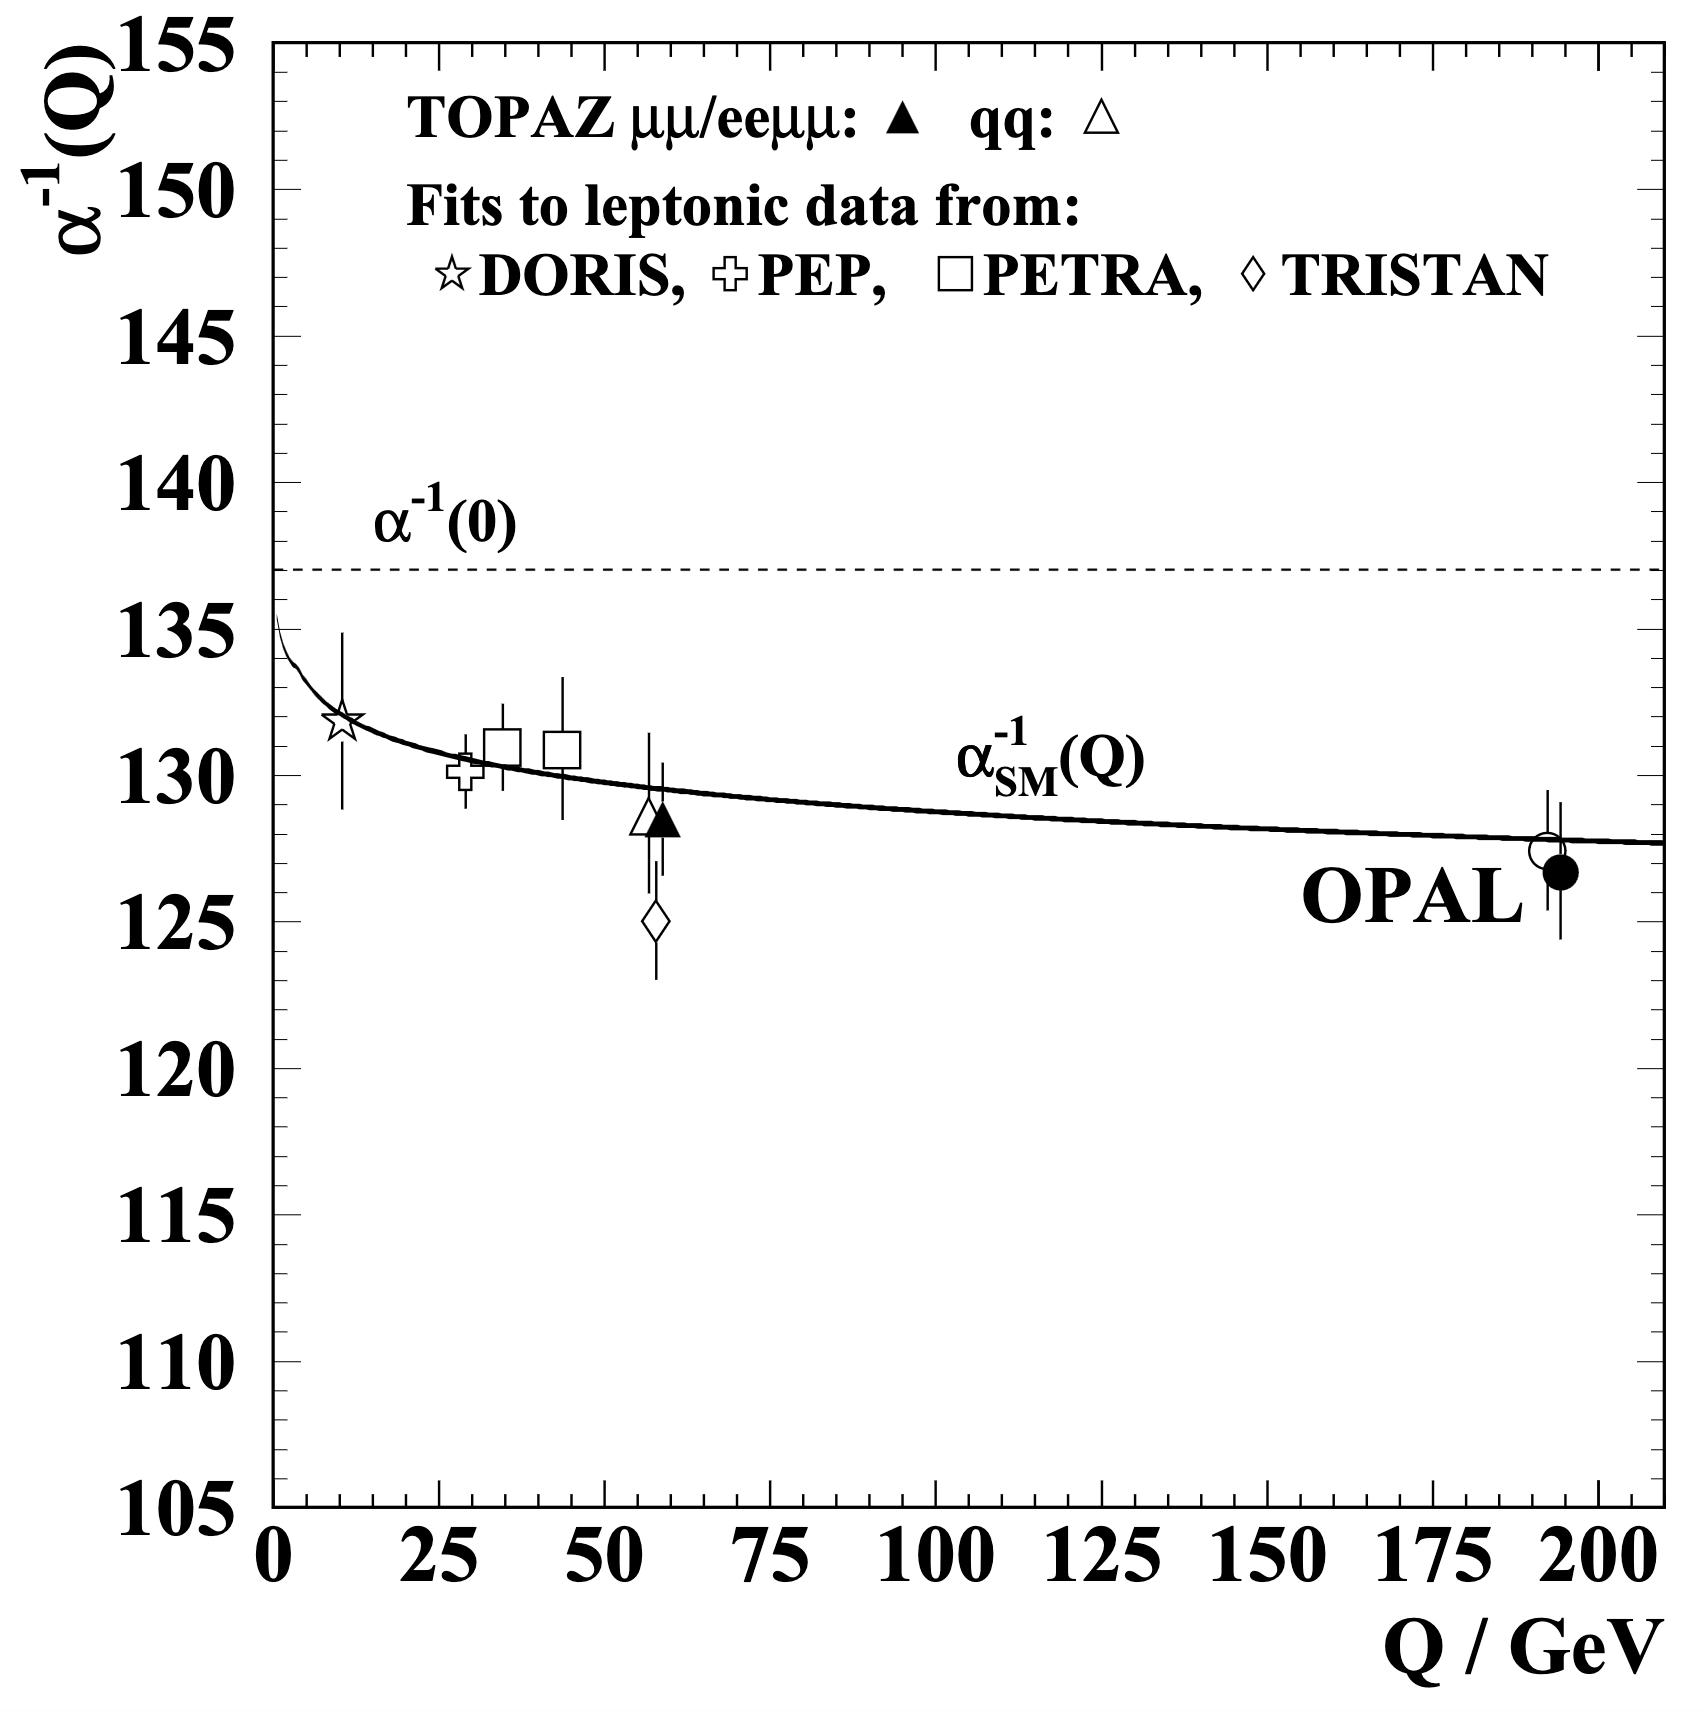
\includegraphics[width=.47\textwidth]{qed_scaling_experiment}}\hspace{5mm}
    \subfigure[]{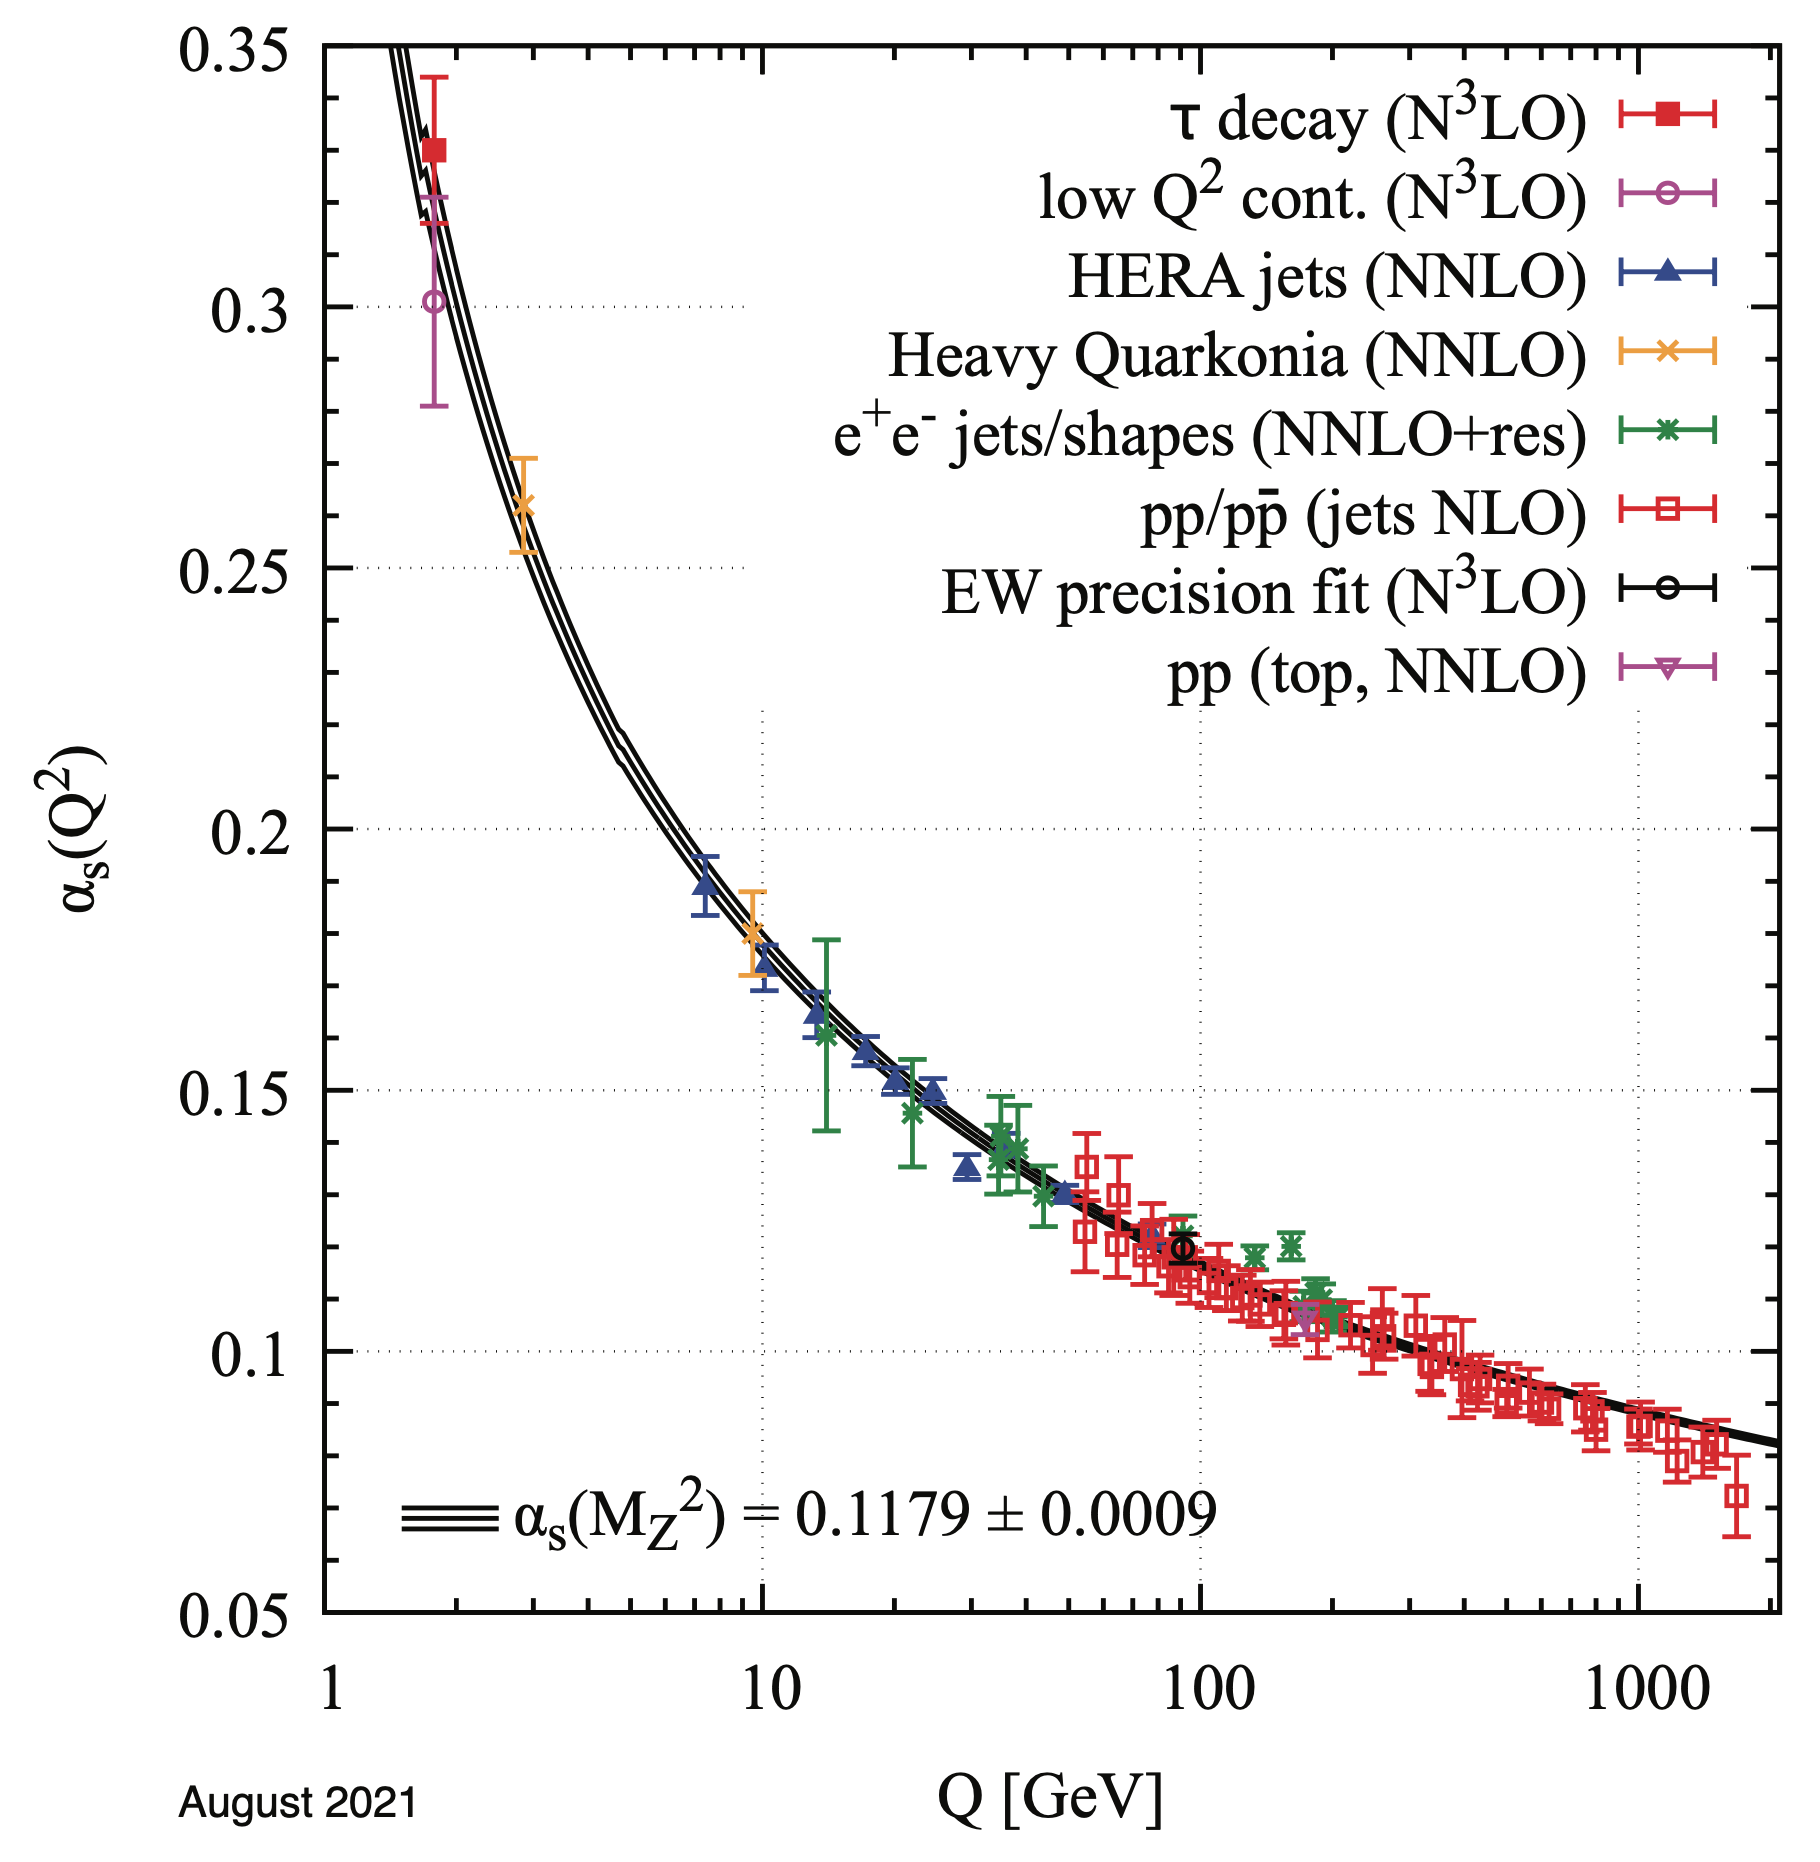
\includegraphics[width=.47\textwidth]{qcd_scaling_experiment}}
    \caption[]{Measurements of the running couplings for (\textbf{a}) \ac{qed} (note the inverted coupling on the y-axis) adopted from \citep{opal2004tests} and (\textbf{b}) \ac{qcd} adopted from \citep{particle2022review}.}
    \label{fig:renorm_scaling_exp}
\end{figure}
Most importantly the running coupling of \ac{qed} does not impact the perturbative approach outlined in section \ref{sec:qft} since $\alpha\ll1$. This is not the case for \ac{qcd} where $\alpha_S$ at $q\approx\qty{1}{GeV}$ is of $\mathcal{O}(1)$. In such scenarios, perturbation theory is ineffective because the expansion in $\alpha_S$ with only one leading term is a poor approximation for calculations of bound hadronic states and later processes in hadronization, as explained below. While perturbation theory for \ac{qcd} remains valid for $\alpha_S\sim  0.1$, which corresponds to $q\gtrsim \qty{100}{GeV}$, for basically all \ac{qcd} calculations at the \ac{lhc}, higher order corrections must be considered.

The behavior of the running coupling in \ac{qcd} is called asymptotic freedom, since the theory is free of asymptotics/divergences with increasing energy scale or decreasing distance. In turn to the photon in \ac{qed}, gluons carry charge and thus attempting to separate quarks results in additional gluons contributions to the interaction, increasing both the energy and force between the quarks. Eventually, it becomes energetically favorable to create a quark-antiquark pair from the vacuum, which then bind with the separating quarks to form new, color-neutral hadrons. This is also known as color confinement, which states that colored particles can only be observed in bound states.

Renormalization is a crucial procedure for ensuring the consistency and predictive power of the \ac{sm} and is also applicable to the electroweak sector. However the complexity of this topic goes beyond the scope of this thesis.


\section{Physics Beyond the Standard Model}\label{sec:beyond_sm}
The \ac{sm} works within its realm but is inherently incomplete given other observed phenomena of which a few are presented here. Most importantly there is no quantum theory for gravity and is thus not part of the \ac{sm}.

Furthermore there is evidence through gravitational effects which cannot be explained by the amounts of ordinary matter which is referred to as dark matter \citep{dark_matter_a_primer}. Furthermore there are several observations showing an accelerated expansion of the universe which is referred to as dark energy \citep{RevModPhys.75.559}. The standard model of cosmology Lambda-Cold Dark Matter ($\Lambda$CDM) \citep{planck2020} models the cosmic microwave background by incorporating dark matter and dark energy with high precision for both of which the \ac{sm} offers no explanation.

Furthermore neutrinos are known to be massive. In principle they can be added like fermions as in the section on the fermion Yukawa mass term \ref{sec:yukawa_term} but this requires right-handed neutrinos which have not been observed. This suggests, since their masses are much smaller than for the other fermions that there might be another mechanism responsible for the generation of the mass of neutrinos.

Moreover, in the standard cosmological model, matter and antimatter should have been created in equal amounts, yet the universe is predominantly made of matter. An explanation of this behavior can be given through the nature of \ac{eswb}. The Sakharov conditions necessary to create the observed baryon asymmetry can be created if \ac{ewsb} is a first order phase transition. In such a transition the position of the minimum in the potential changes abruptly when the universe cools below temperature where \ac{ewsb} occurs as depicted in figure \ref{fig:higgs_phase_transition} \citep{Banerjee2011ElectroweakPT,MICCO2020100045}. 

This phase transition is dictated by the Higgs potential. The assumed form and the measured mass of the \ac{sm} Higgs do not support a first-order phase transition but rather a smooth crossover transition similar to a second order phase transition also shown schematically in figure \ref{fig:higgs_phase_transition} \citep{PhysRevD.105.095041,MICCO2020100045}. The nature of the very early universe is thus inscribed in the shape of the Higgs potential and if we are in an absolute miminum remains unclear as only the mass term of the Higgs potential from equation \ref{eq:higgs_potential} is determined by experiment and only the simplest thinkable potential shape is used to render weak gauges bosons massive. 

\begin{figure}
    \centering
    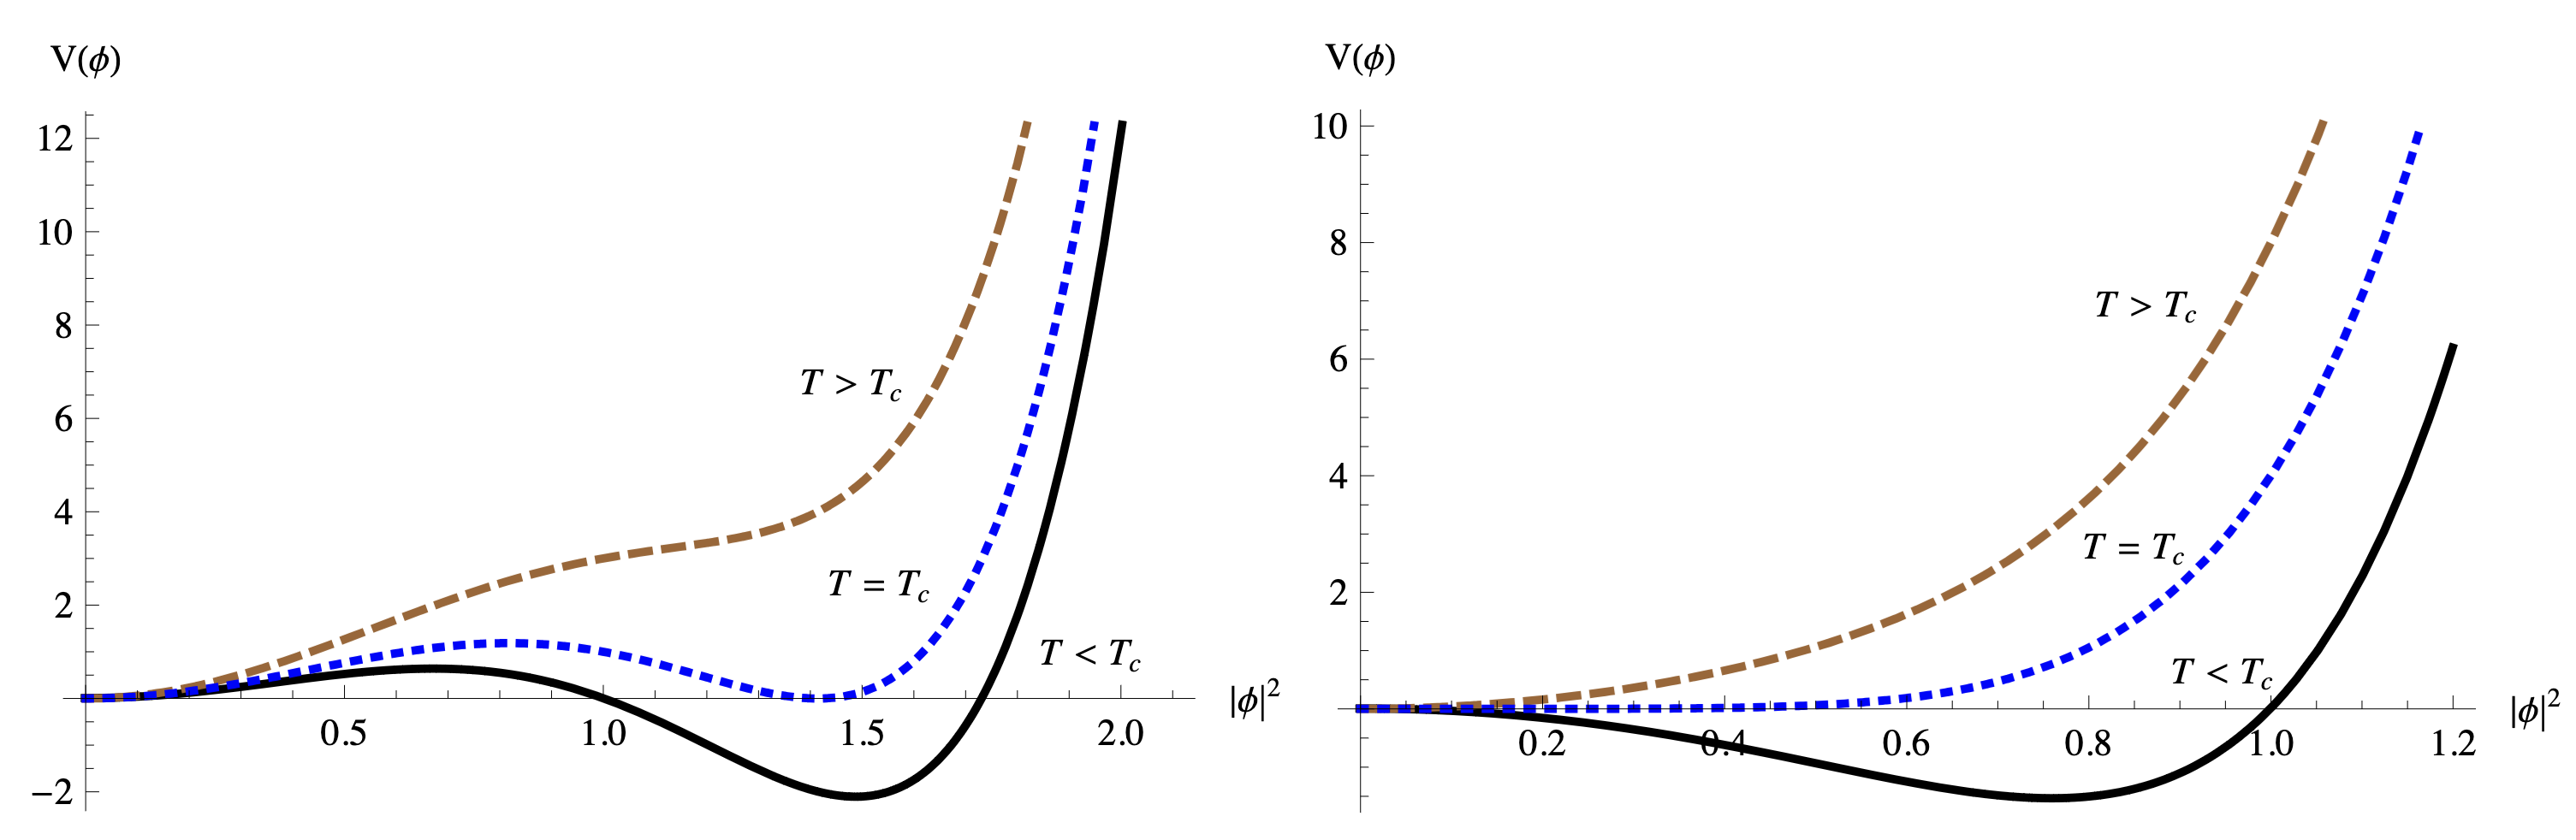
\includegraphics[width=1\textwidth]{higgs_phase_transition}
    \caption[]{(Left) First order phase transition for a given temperature with a sudden change of the minum when the temperature drops below $T_c$, where for (right) a second order phase transition the minimum changes continuously. Adopted from \citep{Banerjee2011ElectroweakPT}.}
    \label{fig:higgs_phase_transition}
\end{figure}

When considering top-quark loop corrections to the Higgs field, as illustrated in figure \ref{fig:top_loop}, the $\lambda(\mu)$ parameter in the Higgs potential becomes energy scale-dependent and allows to make some statements about the shape of the Higgs potential. At an instability energy scale of $\Lambda_I\approx \qty[]{e10}{GeV}$, $\lambda(\mu)$ could turn negative, suggesting that the current \ac{vev} might not be the absolute minimum of the Higgs potential but could be energetically lower or even unbounded \citep{devoto2022false}.


\begin{figure}
    \centering
    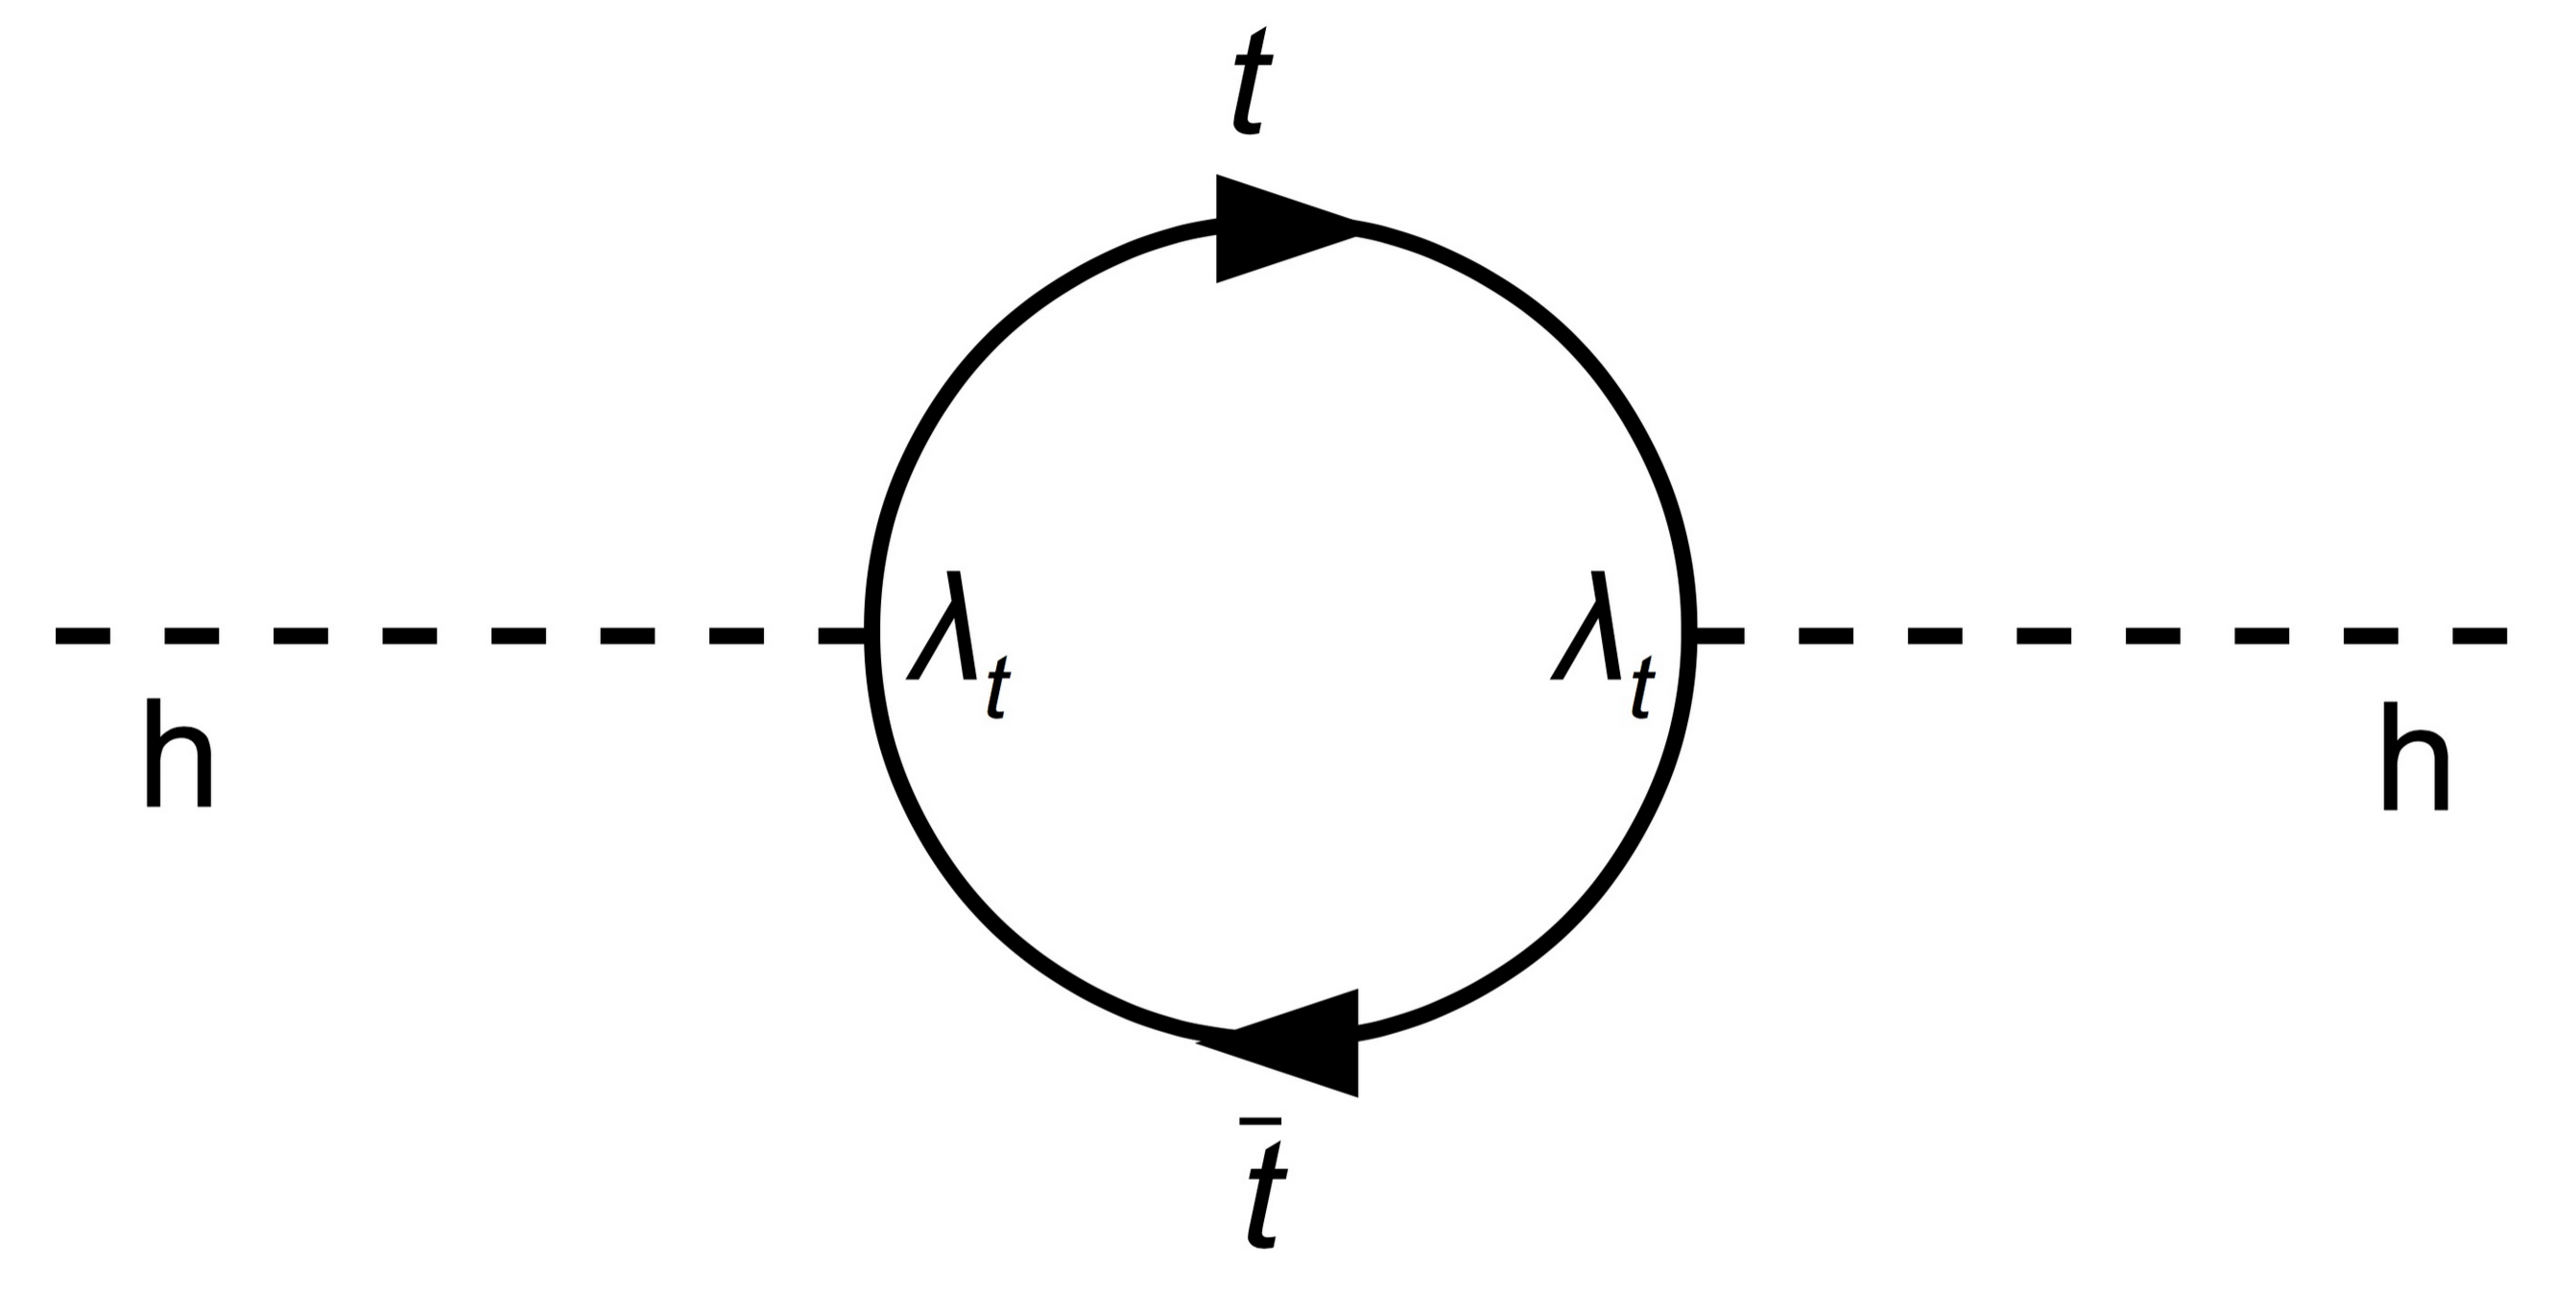
\includegraphics[width=0.35\textwidth]{top_loop}
    \caption[]{Leading correction to the Higgs field from top pair interaction. cite(https://onlinelibrary.wiley.com/doi/pdf/10.1155/2011/968283)}
    \label{fig:top_loop}
\end{figure}


A phase transition via quantum tunneling into a different \ac{vev} could result in the universe's particles, forces and structures ceasing to exist and being replaced by different ones. The stability of the universe, under the assumptions of \ac{sm} physics, critically depends on the precise values of the Higgs and top quark masses, as depicted in the phase diagram in figure \ref{fig:vev_stability}, which places the universe at the boundary between stability and metastability given current measurement accuracies.


\begin{figure}
    \centering
    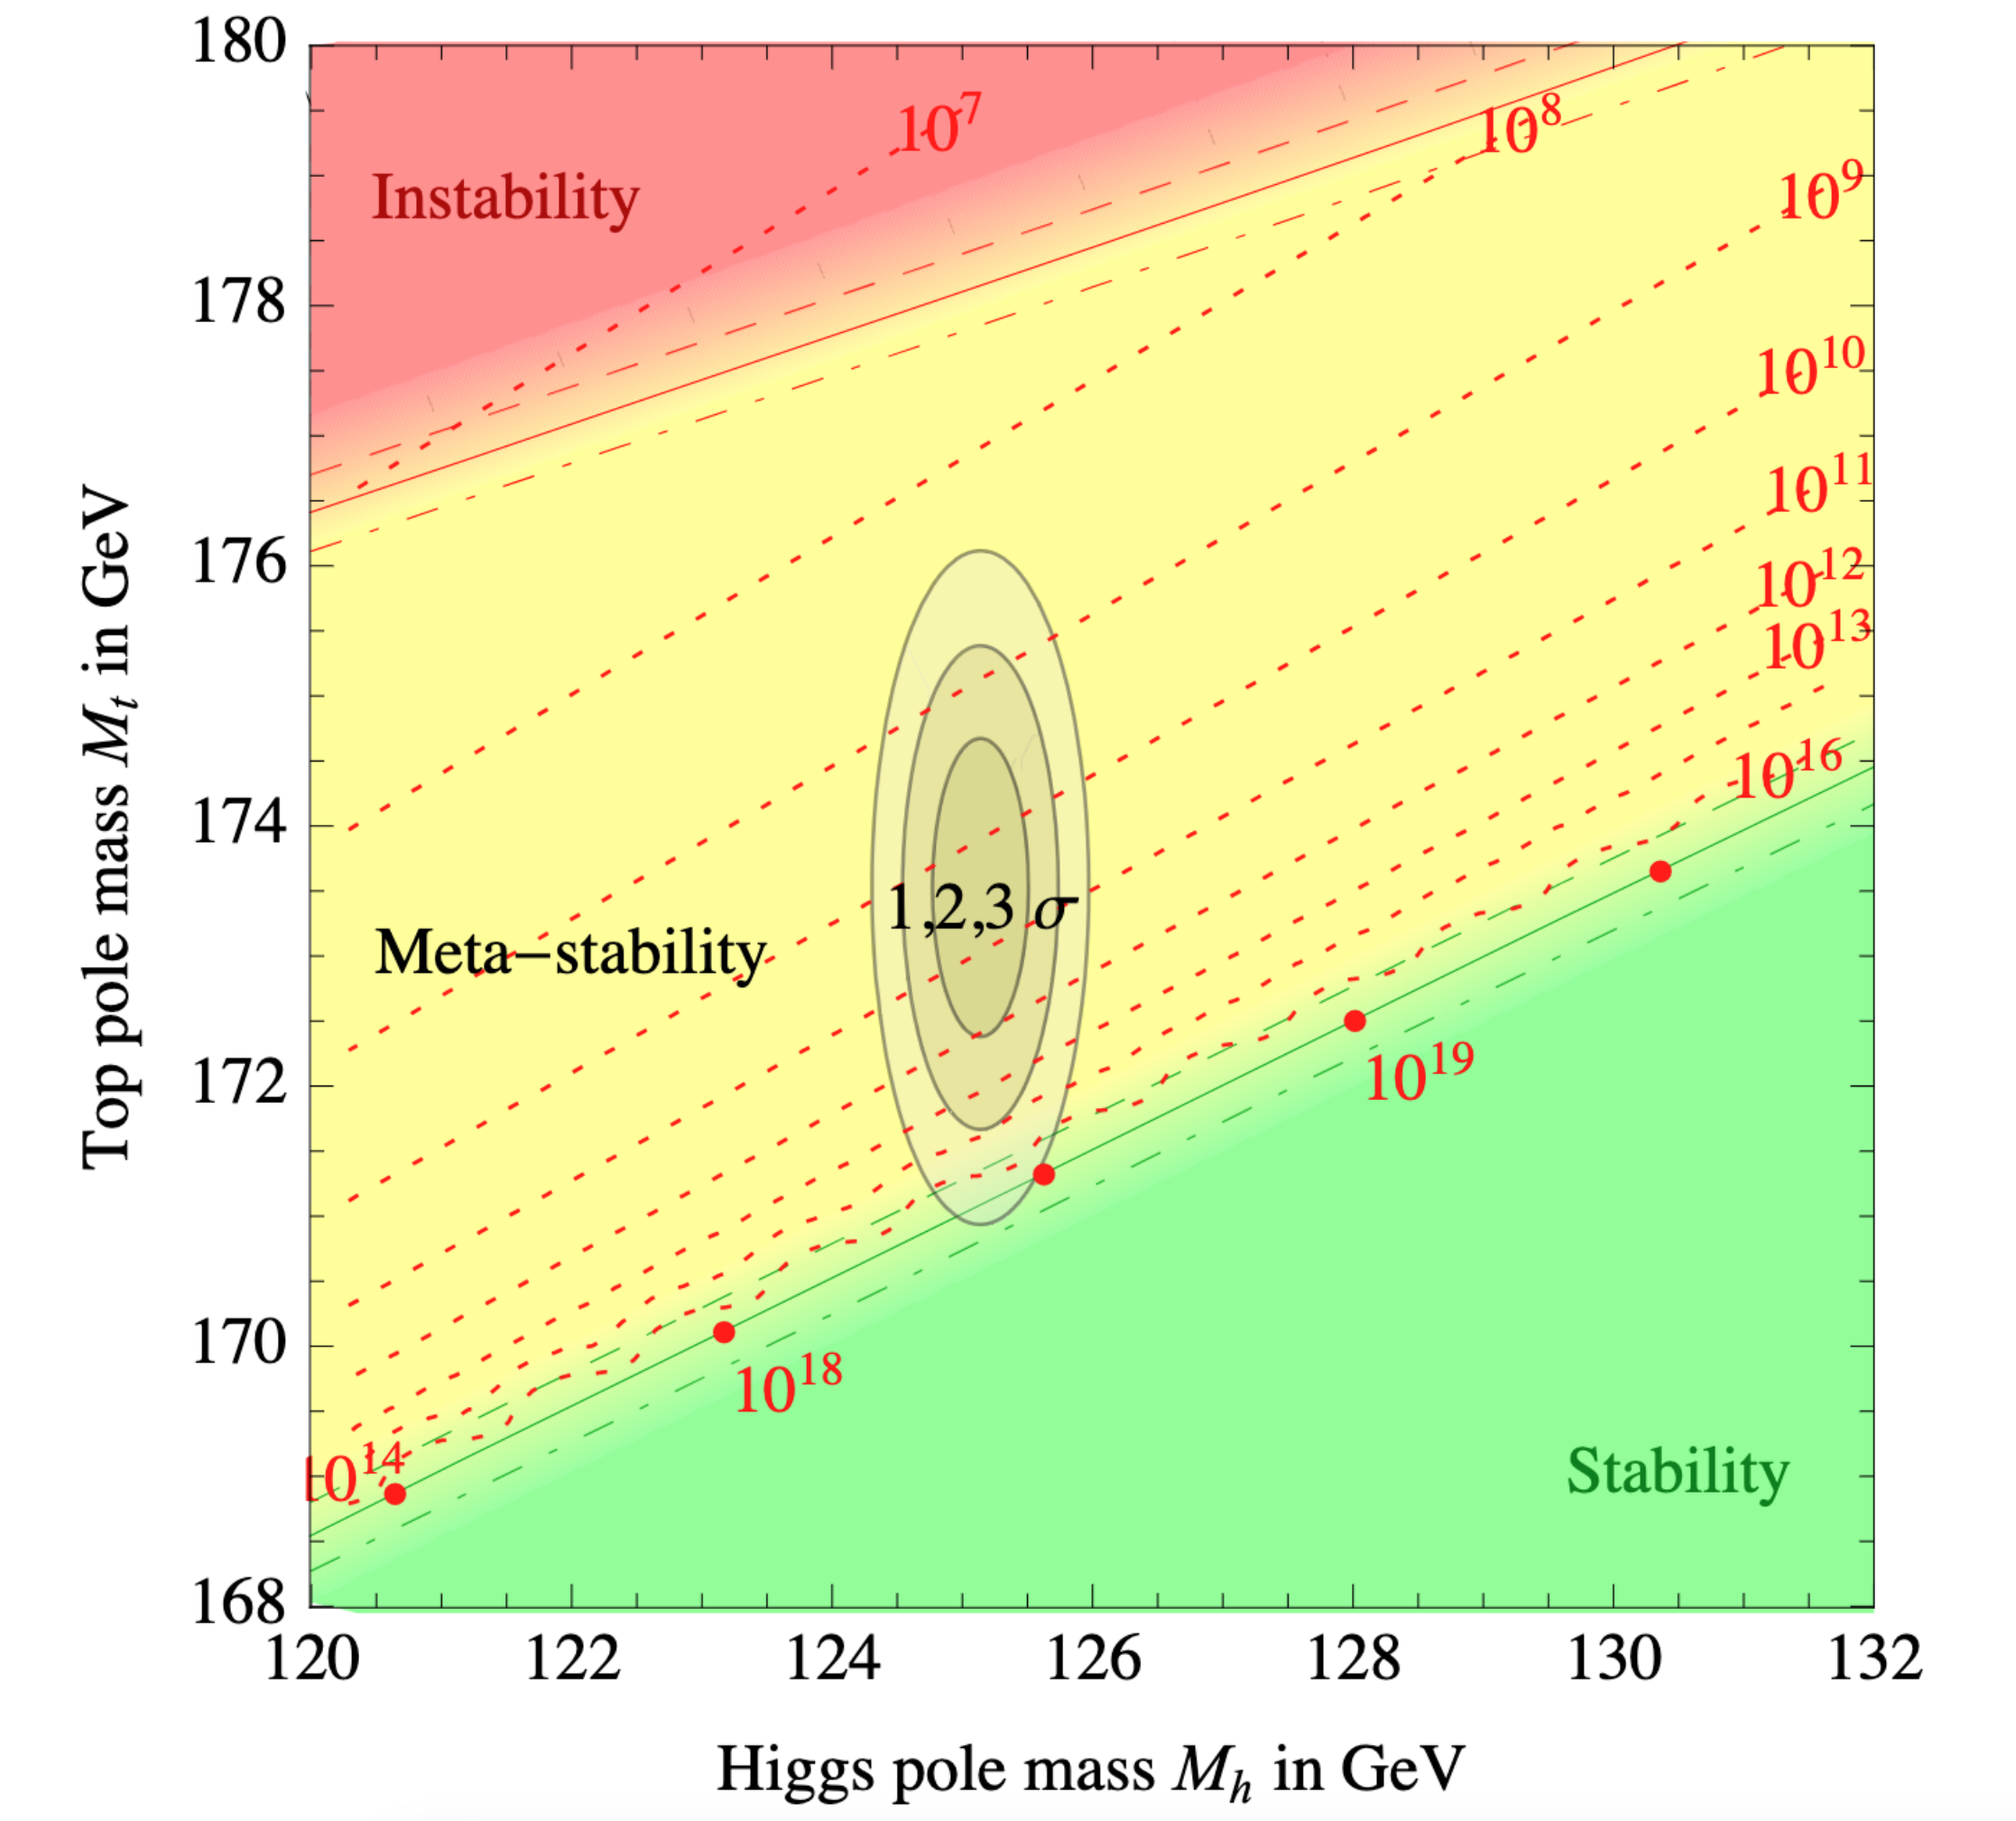
\includegraphics[width=0.7\textwidth]{vev_stability}
    \caption[]{Phase diagram of the stability of the universe assuming the \ac{sm} as a function of the Higgs and top pole masses. Instability for the Higgs potential occurs when due to quantum loop corrections the Higgs field develops a different minimum. Meta-stability is the case when there is an even lower global minimum in the potential and Stability means that there is only one global minimum. The red isolines correspond to the energy scale $\Lambda_I$ at which the Higgs potential becomes unstable. Adopted from \citep{Buttazzo:2013uya}.}
    \label{fig:vev_stability}
\end{figure}





Through the Higgs mechanism, elementary particles gain mass by interacting with the Higgs field. Accurate measurements of properties such as the mass and decay channels of the Higgs boson and the top quark offer means to validate and challenge the \ac{sm}. A precise understanding of these is crucial as any deviation from the expected values could indicate new physics. Moreover, the stability of our universe might be related to these properties. The study of the Higgs potential is therefore a promising endeavor to which this work aims to contribute.


% \chapter{The ATLAS experiment at the Large Hadron Collider}\label{sec:atlas}
Exploring the nature of the Higgs particle requires collision energies on the \qty[]{}{TeV} scale. The \ac{lhc} is currently the most powerful particle accelerator making it the best available facility for studying the Higgs particle. The main reference for this section is \citep{aad2008atlas}.

\section{The Large Hadron Collider}
The \ac{lhc} is a circular proton proton collider with \qty[]{27}{km} circumference with a center-of-mass energy of $\sqrt{s}=\qty[]{13}{TeV}$. The two anticyclic proton beams are actually bunches containing $10^{11}$ protons that are brought to collisions at several points of the ring for the experiments performed at the \ac{lhc}. A measure of how tightly particles are packed in these bunches is the instantaneous luminosity and is characteristic to the collider
\begin{equation}
    L=\frac{1}{\sigma}\frac{\dint{N}}{\dint{t}}.
\end{equation}
It can be read as particle interactions per unit time and area. The area understood as the interaction cross-section of a particular process. The total recorded number of collision events can thus be calculated by summing the luminosity over time which gives with the integrated luminosity
\begin{equation}
    N=\sigma\cdot\int L dt=\sigma\cdot L_\mathrm{int}.
\end{equation}
For the full run 2 dataset used in this thesis the integrated luminosity for events good for physics analysis is \qty[]{140.1}{fb^{-1}} \citep{DAPR-2021-01}.

\section{The ATLAS detector}
The \ac{atlas} (A Toroidal LHC Apparatus) experiment is a particle detector with an onion-like structure, as shown in figure \ref{fig:atlas_detector}.
\begin{figure}
    \centering
    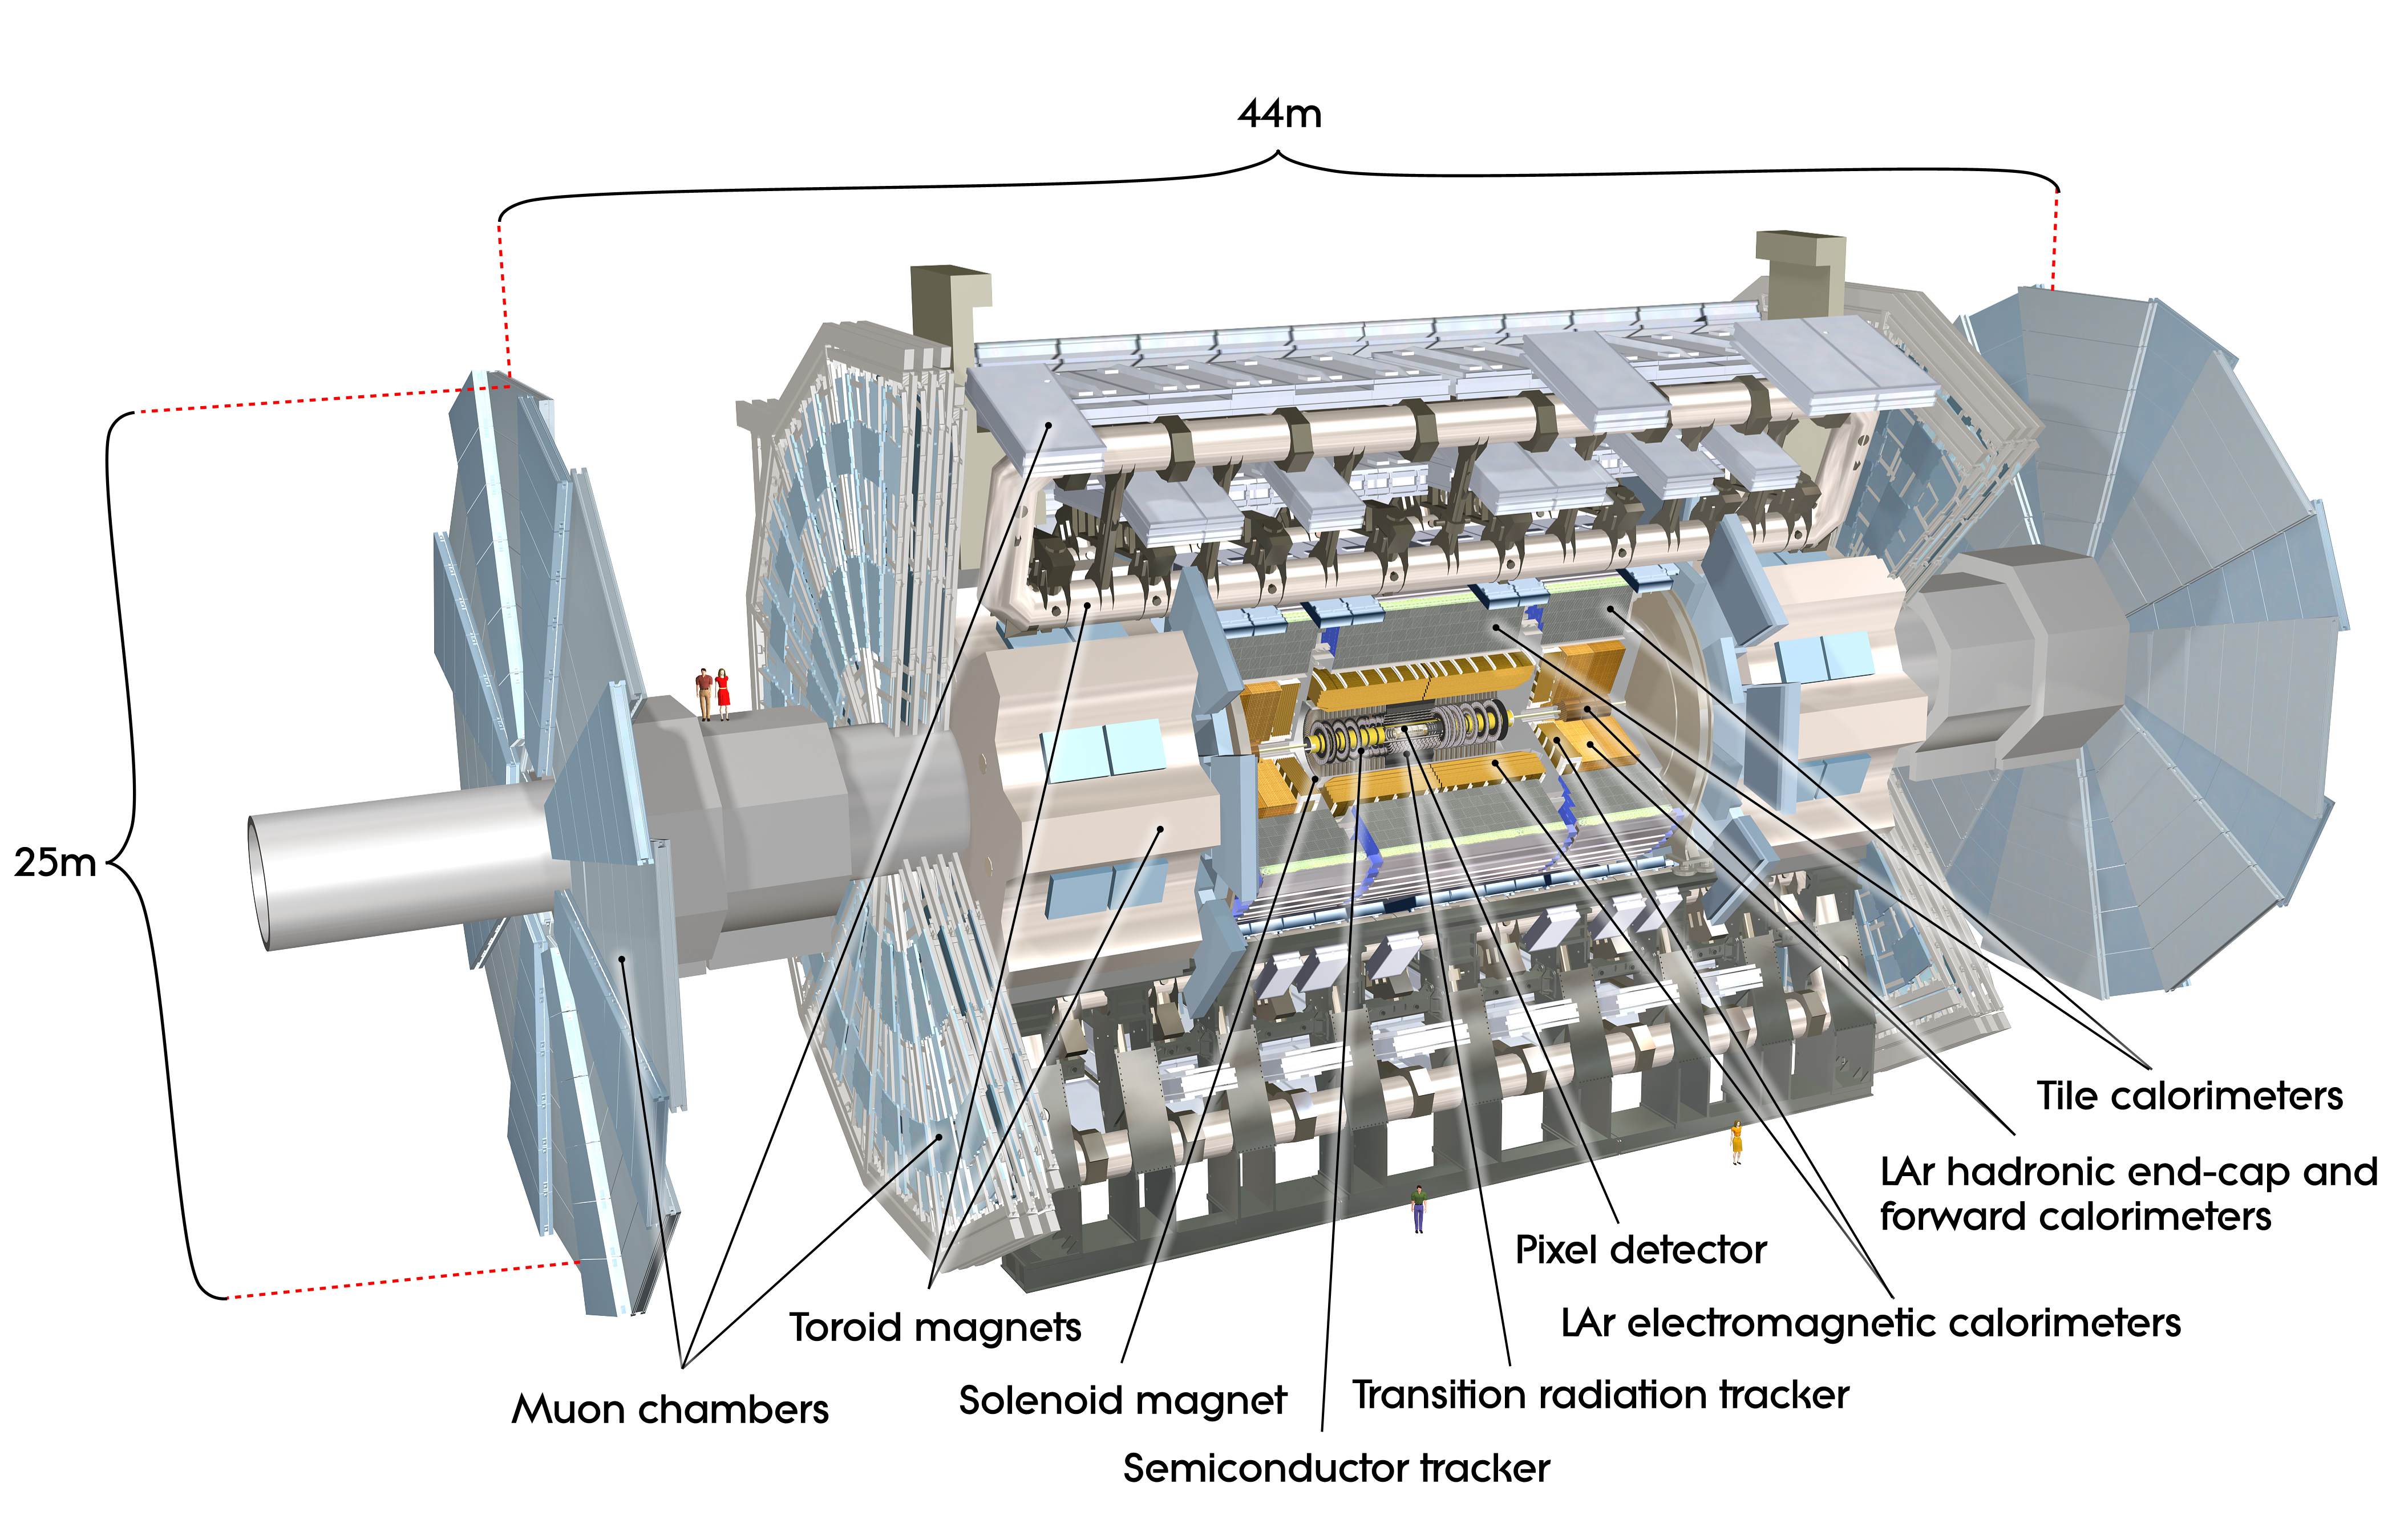
\includegraphics[width=1\textwidth]{atlas_detector}
    \caption[]{The \ac{atlas} experiment at the \ac{lhc} with its subdetectors. Adopted from \citep{Pequenao:1095924}.}
    \label{fig:atlas_detector}
\end{figure}
Its purpose is to measure the trajectory, momentum, and energy of particles originating from proton-proton collisions, depending on the particular kind of interaction of the collision products with matter. The various subdetectors are explained below from the inside out.

\subsection*{Coordinate System}
The coordinate system of \ac{atlas} is right-handed and originates at the interaction point at the center of the detector. The z-axis points along the beam line, the x-axis to the center of the lhc and the y-axis away from earth. Thus quantities transversal to the z-axis are Lorentz-invariant. Inside the detector cylindrical coordinates $r,\phi$ are used with $\phi$ the azimuthal angle about the z-axis and the polar angle $\Theta$ of a particle measured in form of the pseudorapidity $\eta=-\ln(\Theta/2)$. This quantity is defined as an approximation for the Lorentz invariant rapidity and holds for highly relativistic particles. With these a useful quantity to describe angular distances in the detector is
\begin{equation}
    \Delta R = \sqrt{(\Delta\phi)^2+(\Delta \eta)^2}.
    \label{eq:delta_R}
\end{equation}

\section{Inner detector}\label{sec:inner_detector}
The inner detector, shown schematically in figure \ref{fig:inner_tracker}, is designed to track charged particles and figure out their momentum and provide information on the particle type.
\begin{figure}
    \centering
    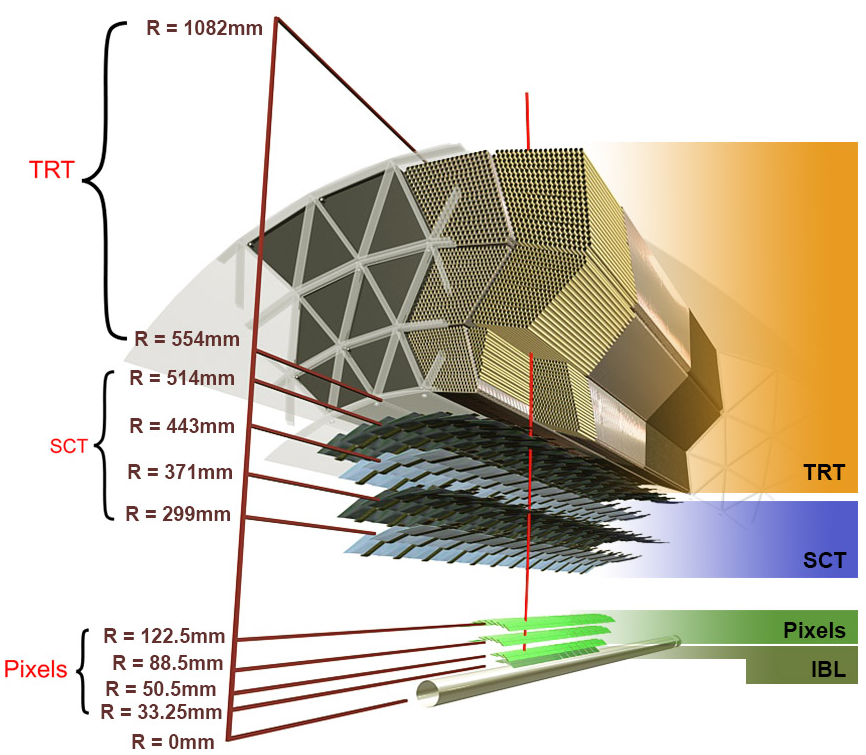
\includegraphics[width=0.65\textwidth]{inner_tracker}
    \caption[]{The inner detector schematically with the subdetectors described in the full text. Adopted from \citep{Potamianos:2016ptf}.}
    \label{fig:inner_tracker}
\end{figure}
It is surrounded by a solenoid magnet whose field lines point in the direction the beam so that charged particles are bent in the transverse plane of the detector due to the Lorentz force. The bending direction reveals the charge whereas the curvature depends on the momentum.

The \ac{ibl}, pixel detector, and \ac{sct} all consist of silicon detectors of various sizes. When passing through silicon, charged particles ionize electrons that travel in an electric field to an electrode and provide positional information. The \ac{ibl} plays a crucial role in b-tagging as will become clear in section \ref{sec:b_tagging}.

Aforementioned semiconductor trackers are surrounded by the \ac{trt} which apart from tracking also can identify particles. It consists of several layers of tubes perpendicular to the beamline, filled with a gas mixture, and a conducting wire in their center, which is under voltage and attracts negative charges. The tubes are surrounded in a material with different permittivity so that charged particles passing through the boundaries of the material emit transition radiation. The intensity of this radiation depends on the velocity, so that for particles of the same energy more photons are released for the lighter particle. Therefore for electrons for example can be distinguished from pions.

\section{Calorimeters}

When high-energy particles pass through dense matter the various particle interactions create secondary particles that result in a particle shower. Via this the energy of particles can be inferred and is done in \ac{atlas} with two sampling calorimeters. These consist of alternating layers of a high-density metal to absorb the energy and a material that can track the particles of the shower.

\subsection*{Electromagnetic Calorimeter}

In the electromagnetic calorimeter the main energy deposits are from electrons and photons. The stopping material consists of lead and steel and is alternated with a copper plate on which there is an electrode grid. Between the plates is liquid argon. When interacting with the dense metal e.g. by bremsstrahlung of an electron or by pair production induced by a photon, the created secondary particles ionize the argon atoms in between. The negatively charged ions are then pulled to the charged copper electrodes to determine the position. From the distance a particle has traveled through the electromagnetic calorimeter, one can infer the energy of the particle as it entered the calorimeter.

\subsection*{Hadronic Calorimeter}

Hadrons also deposit energy in the electromagnetic calorimeter but interact with nuclei as well. However as they are more energetic more stopping power is needed which is provided by the hadronic calorimeter that surrounds the electromagnetic calorimeter. The configuration is made of many layers of tiles positioned in planes perpendicular to the beamline. In these layers tiles of steel as stopping material alternate by a scintillating plastic which radiates light if charged particles pass through. The light is collected at the edges by wavelength-shifting optical fibres  which reduce the energy of the photons and then read out by photomultiplier tubes.

\section{Muon Spectrometer}

The muon spectrometer encircles all other detectors to capture muons which barely loose energy passing through the other detectors. Its basic units are resistive plate chambers in three layers around the calorimeters. These are basically large charged capacitors filled with gas. When charged particles pass through they ionize the gas and the resulting avalanche of ions drawn to the electrodes is measured to determine the position and time of flight through the plates.  In addition, they are also used in a design where the electrodes consist of a tube filled with gas and a wire inside similar to the \ac{trt}. The entire spectrometer is placed in a toroidal magnetic field so that the field lines are in phi direction in order to also measure the momentum due to the curvature of the muons.

The figure \ref{fig:particles_in_detector} shows where which type of particles are stopped in the different detectors.
\begin{figure}
    \centering
    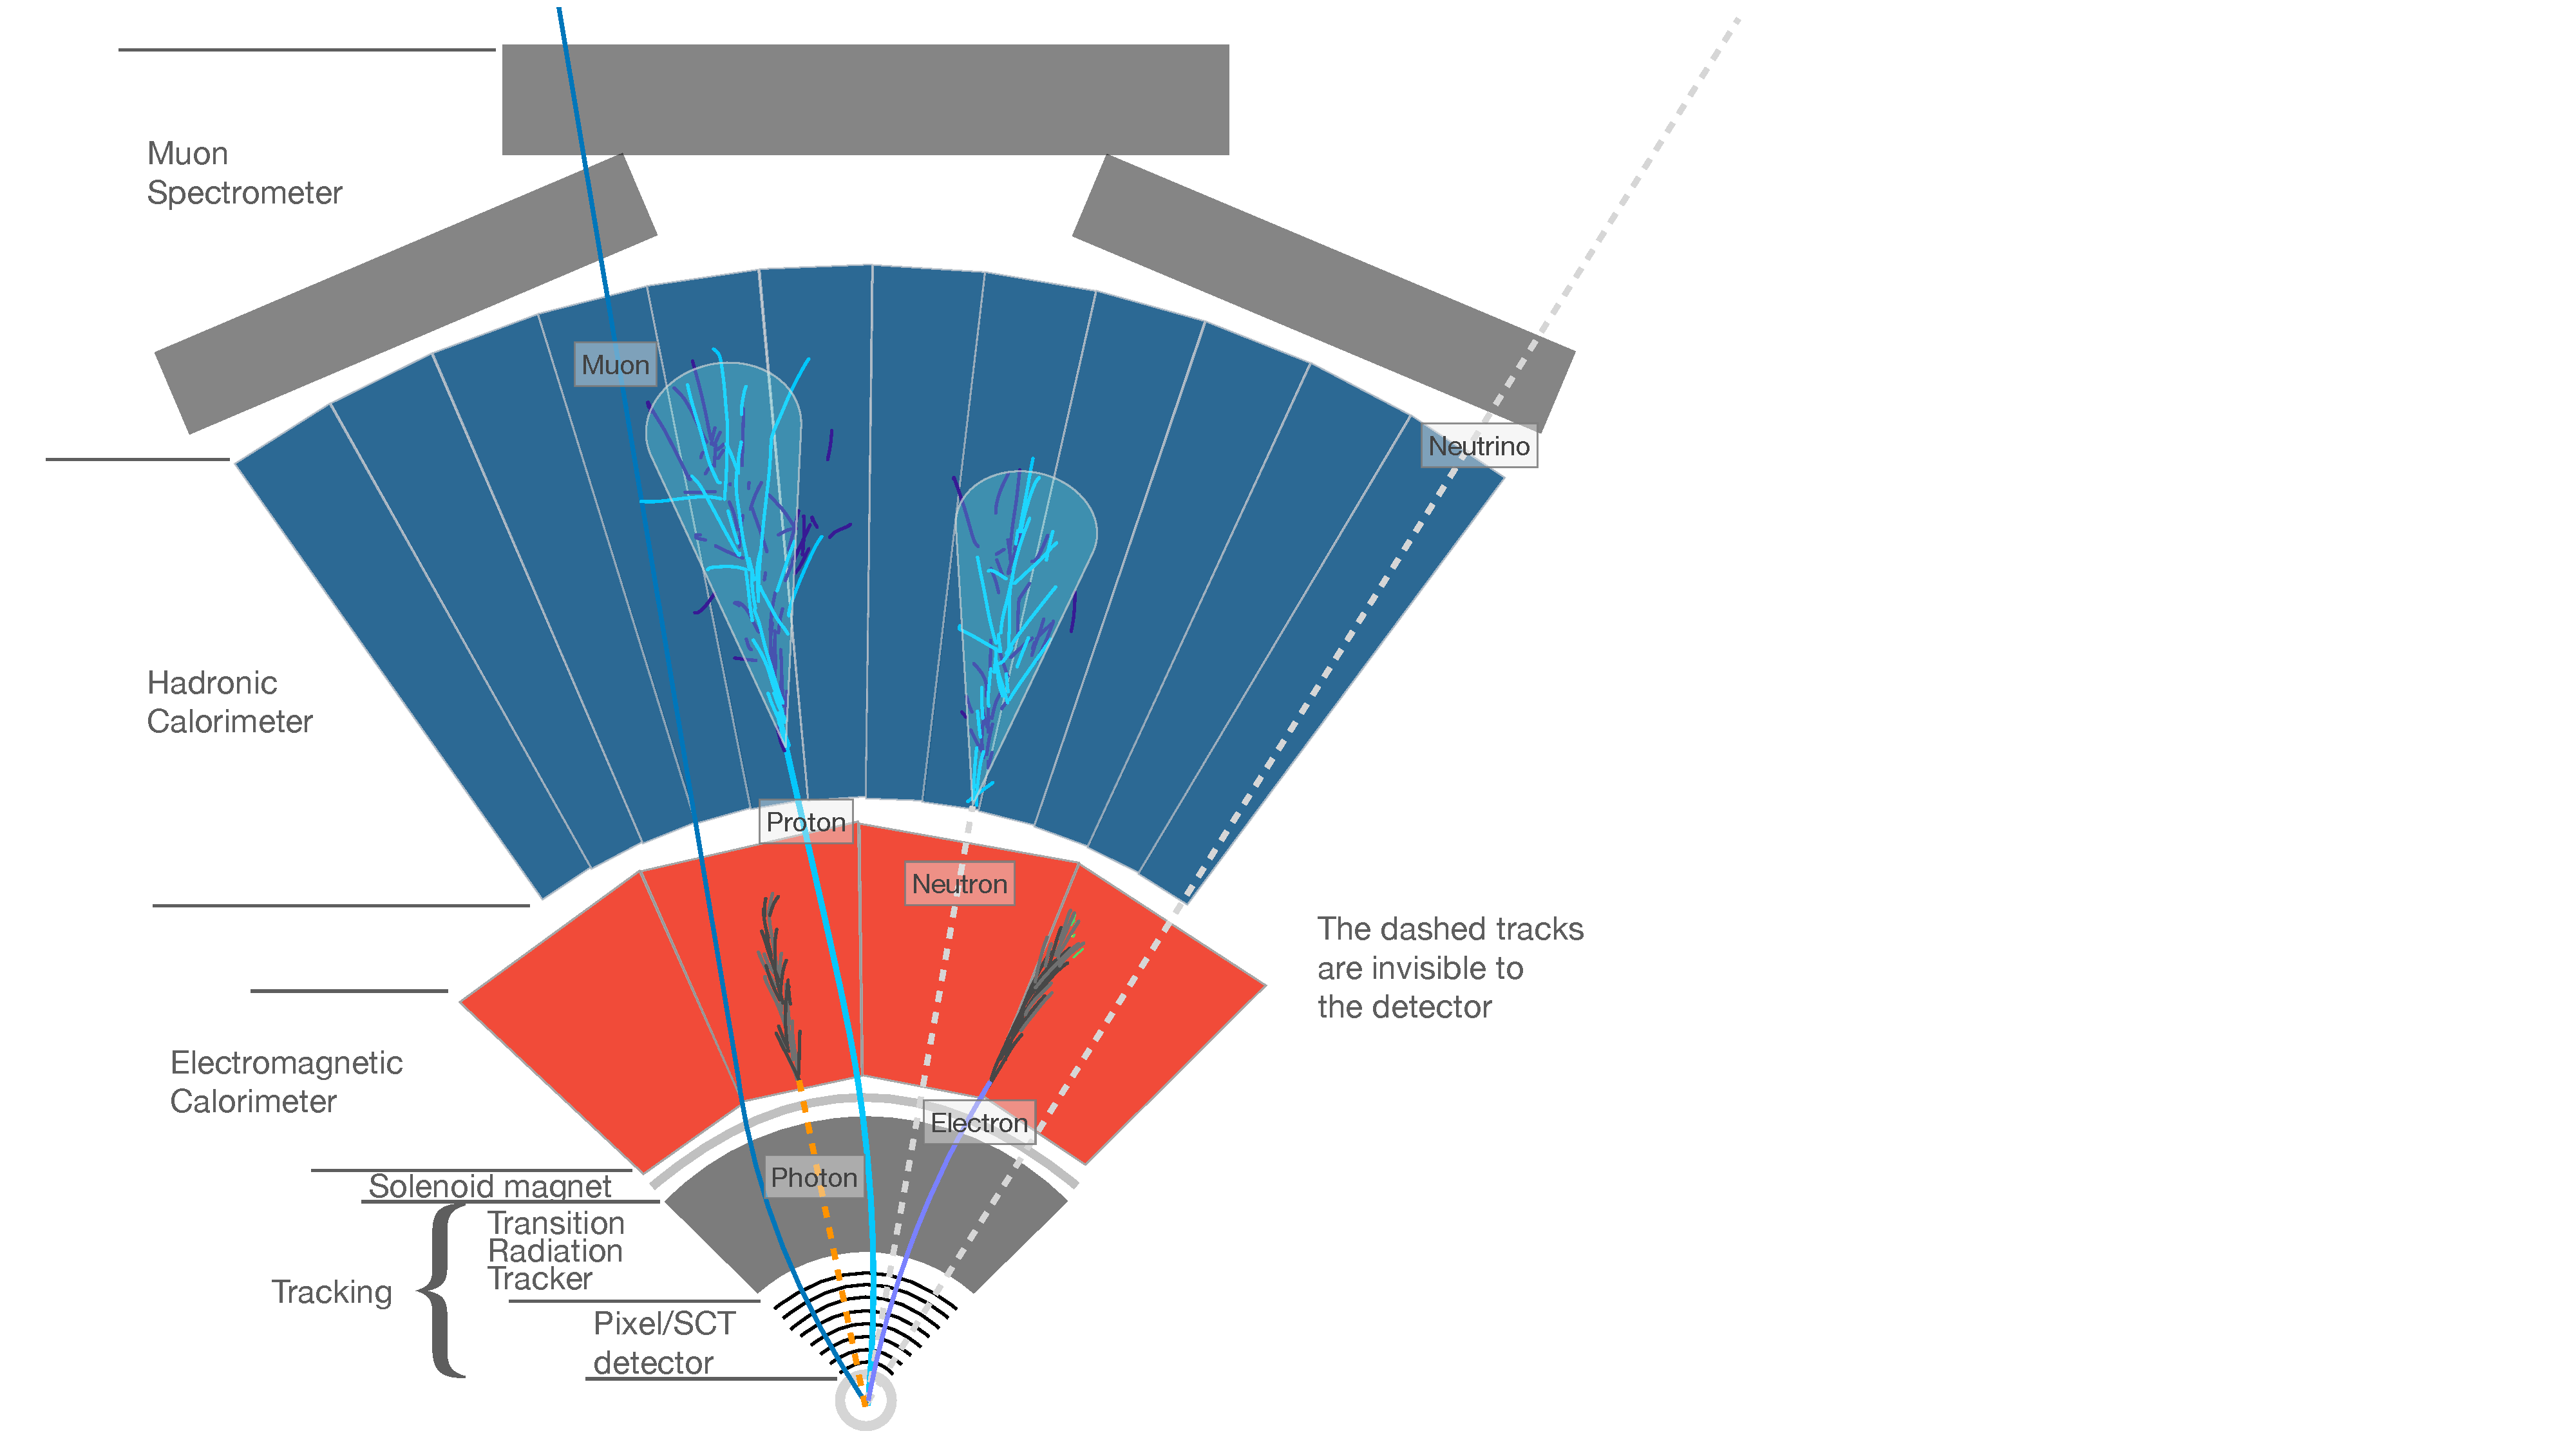
\includegraphics[width=1\textwidth]{particle-shower}
    \caption[]{Paths and energy deposits of particle types in the subdetectors. Adopted from \citep{Guth:2765038}.}
    \label{fig:particles_in_detector}
\end{figure}

\section{Data Acquisition}\label{sec:tdaq}
Bunches of protons in the \ac{lhc} are brought to collision in \ac{atlas} with a rate of \qty[]{40}{MHz}. It is technically impossible at the moment to record all collisions as this would correspond to a data rate of \qty[]{40}{TB\per s}. Therefore events that are useful for physics analysis need to be preselected which is called triggering and is performed in two steps. The first step is the \ac{l1} trigger and is hardware based and reduces the event rate to \qty[]{100}{kHZ}. This is done by selecting events with large transverse momentum deposits in the detector and also for events with missing transverse momentum. Afterwards the regions in the detector where this is the case are passed to a software \ac{hlt}. This then uses the full detector information in these regions to reduce the rate further down to \qty[]{1}{kHz}.

% \part{Methodology}
% \chapter{Physical Object Reconstruction}\label{ch:reco}

Physical properties of particles produced from a collision at the \ac{lhc} is derived by combining the traces these particles leave in the various subdetectors on their way through \ac{atlas}. This  reconstruction is described in the following for objects used in this analysis. The main resource for this chapter is \citep{atlas2021optimisation}.

\section{Tracks and Primary Vertex}\label{sec:tracks}
Charged particles leave a trajectory in the \ac{id} as explained in the section \ref{sec:inner_detector}. To reconstruct the path of these particles an algorithm first groups hits that are close to each other in the silicon detectors into clusters. These clusters are then successively combined to determine the most probable trajectory that the particles have taken through the detector which are referred to as tracks \citep{aaboud2017performance}. These are then geometrically matched to proton-proton interactions and the vertex with the largest scalar sum of transverse momentum $\sum \pt^2$ becomes the primary hard scatter vertex. In addition, the momentum is also determined based on the curvature of the particle through the magnetic field and at least two tracks with $\pt>\qty[]{500}{MeV}$ are required in the tracking volume $\abs{\eta}<2.5$.

\section{Jets}\label{sec:jets}
As explained in section \ref{sec:renormalization} quarks cannot be observed individually but only as colorless hadrons. When decaying they undergo showering and hadronization forming cone-like structures of energy deposits in the detector called jets. They are reconstructed by combining tracking and calorimeter information.

\subsection{Topocluster}
For that purpose the deposited energy of these decays in the calorimeters are grouped three-dimensionally by combining calorimeter cells into so-called topoclusters. These clusters are seeded from cells that display a signal stronger than four times the standard deviation of detector noise $4\sigma_\mathrm{noise}$ and is complemented by $2\sigma_\mathrm{noise}$ cells.

\subsection{Particle Flow Object}
The energy and mass resolution calculated from these clusters can be improved by geometrically matching tracks to the clusters. If a track is matched successfully to a topocluster the energy of the track and the position in the calorimeter is used to infer the energy of the particle that created the track. From this expected energy all associated cluster cell energies are subtracted and the remnant is removed from the expected energy if the deviation corresponds to energies of the order of typical fluctuations. Such combination of a topocluster and a track are called \ac{pfo} \citep{aaboud2017jet}. Sometimes energy of one track ends up in several clusters. For this the Particle Flow algorithm combines the most probable clusters with the track. Topoclusters without matched tracks are assumed to be neutral particles as they do not leave a trace in the \ac{id}. \acp{pfo} not matched to the \ac{pv} are removed to reduce the contribution from pileup.

\subsection{Track-CaloClusters}
Instead of using the energy measurement of the tracks as for \acp{pfo} for \ac{tcc} the calorimeter energy measurement is used and complemented by the angular information of the tracks. \ac{tcc} was developed for high \pt jets since the resolution in the calorimeters improves with larger momentum since the calorimeter deposits become more localized.

% \subsection{Unified Flow Object}
% Particle Flow benefits from the momentum/energy resolution of the \ac{id} compared to the calorimeters especially at low momenta. Although this gradually breaks down with increasing momentum and also with particle density because the matching of tracks to clusters becomes more and more ambiguous in that case. \ac{ufo} jets are designed to make the most of both reconstruction algorithms by choosing the algorithm that performs best for the situation at hand.

\subsection{Anti-$k_t$ Jet Clustering Algorithm}\label{sec:anti_kt}
The definition of a jet is not unique as it depends on the size and direction of the cone and thus how many particles are included. For this the Anti-$k_t$ algorithm \citep{cacciari2008anti} clusters aforementioned four vector objects in this section into cone-shaped jets. It starts with calculating the distances between all four vector objects $i,j$ that are considered
\begin{equation}
  d_{ij}=\frac{1}{\max(p_{T,i}^{2}\,,\,p_{T,j}^{2})} \frac{\Delta R_{ij}^2}{R^2},
\end{equation}
and the distance to the beam
\begin{equation}
  d_{iB}=\frac{1}{p_{T,i}^{2}},
\end{equation}
with the transverse momenta of the particles $p_{T,i},p_{T,j}$ their angular distance $\Delta R$ as of equation \ref{eq:delta_R} and a chosen radius parameter $R$. The algorithm combines objects $i,j$ into a new four vector for the smallest distance $d_{ij}$. Since this distance is small for large transverse momentum \pt and small angular distance $\Delta R_{ij}$ the algorithm prefers these accordingly. After combining two object the algorithm starts for as long as $d_{iB}<d_{ij}$. Thus it stops once particles outside of the chosen radius would be added. In \ac{atlas} jets with  a radius parameter of $R=0.4 (1.0)$ are usually denoted as Small-R(Large-R) jets.


\subsection{Variable Radius Jets}\label{sec:vr_jets}
In very boosted regimes mit large momenta individual jets can overlap. In order to still reconstruct them individually a \ac{vr} for the $R$ parameter from the Anti-$k_t$ Jet Clustering Algorithm of section \ref{sec:anti_kt} is used
\begin{equation}
  R\rightarrow R_\text{eff}(\pt)=\frac{\rho}{\pt}
\end{equation}
It becomes therefore dependent on the transverse momentum and is controlled by a parameter $\rho$ so that the jet size decreases with \pt. \ac{vr} jets are reconstructed from tracks and are required to have $\pt>\qty[]{10}{GeV}$.

\section{$b$-tagging}\label{sec:b_tagging}
This analysis has four $b$-quarks in the final state and therefore relies on their identification.  Fortunately, due to their large mass $\tau\sim\qty{1.5}{ps}$, $b$ quarks have a long lifetime compared to other quarks resulting in a path length of about $c\tau\sim\qty{450}{\micro m}$. Even though they do not reach the \ac{id} a secondary vertex is formed at the point where the $b$-hadron decays which can be inferred from the tracks.

Such tracks have a large impact parameter that is defined as the distance of closest approach in the $r-\phi$ projection in transverse $d_0$ and longitudinal $z_o$ direction \citep{aad2008atlas} as illustrated in figure \ref{fig:secondary_vertex}b. Other methods for determining the secondary vertex attempt to connect the tracks of the $b$-hadron decay with those of a subsequent $c$-hadron decay by aligning the tracks in Fig. \ref{fig:secondary_vertex}a and also by deriving the mutual origins of the tracks \citep{ATL-PHYS-PUB-2017-013}.
\begin{figure}[]
  \centering
  \subfigure[]{
    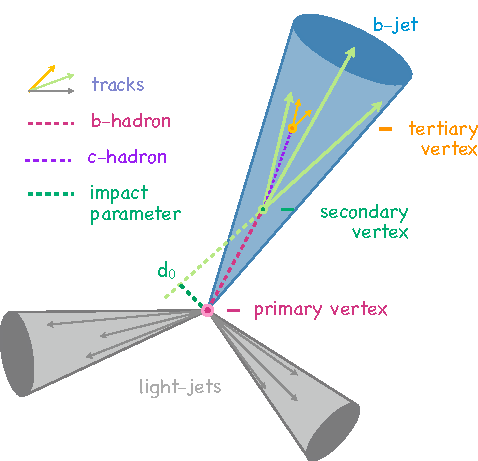
\includegraphics[width=0.49\textwidth]{secVexMguth}
  }%\hspace*{1cm}
  \subfigure[]{
    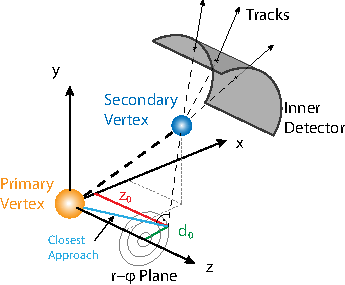
\includegraphics[width=0.49\textwidth]{SV_sketch}
  }
  \caption{(a) Example decay involving a $b$-jet (\hexbox{8AB2D3}) and jets from light flavor hadrons (\hexbox{C5C6C6}). (b) Impact parameters defined for tracks as distance of closest approach to the primary vertex for (\mbox{\color[HTML]{009245}{$d_0$}}) in the $r-\phi$-plane and for (\mbox{\color[HTML]{EC1C25}{$z_0$}}) along the z axis. (a) Adopted from \cite{Guth:2765038}.}
  \label{fig:secondary_vertex}
\end{figure}

\subsection{DL1r Tagger}
The results of the secondary vertex- and impact parameter finding algorithm as well as the jet kinematics are then passed into a deep feed-forward neural network called DL1r which is trained to distinguish $b$-jets from jets of other flavors \citep{atlas2022atlas}. The outputs nodes for flavor classification ($p_\mathrm{b}, p_\mathrm{c}, p_\mathrm{light}$) are further combined into a single discriminating score variable
\begin{equation}
  D_\mathrm{DL1r}=\ln\left(\frac{p_b}{f_c \cdot p_c + (1-f_c)\cdot p_\mathrm{light} }\right).
\end{equation}
$f_c$ is the fraction of charm jets in the background and can be used to tune the importance of the different background classes ($\sum f_\mathrm{bkg} =1$). When evaluating the \ac{nn} a value for the discriminating variable can be derived that corresponds to a $b$-jet selection efficiency which is then applied in physics analysis.

\subsection{$X\rightarrow bb$ Tagger}\label{sec:xbb}
For a collision event where the decay products consists of $b$-jets with large transverse momentum they can overlap. For such cases \ac{vr} track jets from section \ref{sec:vr_jets} can be reconstructed from inside large-$R$ jets that encompass both $b$-jets. The \ac{vr} jets are required to have $\rho=\qty[]{30}{GeV}$ and an allowed radius parameter range of $R_\text{min}=0.02$ and $R_\text{max}=0.4$. These parameters are optimized for Higgs to $bb$ decays \citep{ATL-PHYS-PUB-2017-010} and the \ac{vr} jets are not allowed to overlap.

The $X\rightarrow bb$ tagger is a feed-forward \ac{nn} \citep{ATL-PHYS-PUB-2020-019} that gets as inputs the \pt and $\eta$ of the large-$R$ jet and the output from DL1r for up to three \ac{vr} track jets. Similar to DL1r a discriminant is calculated from the output scores for Higgs, top and multijet decay of the event passed to the \ac{nn}
\begin{equation}
  D_{\text{Xbb}}=\ln\left({\frac{p_{\text{Higgs}}}{f_{\text{top}}\cdot p_{\text{top}}+(1-f_{\text{top}})\cdot p_{\text{multijet}}}}\right).
\end{equation}
$f_\text{top}$ denotes the top fraction with regards to the multijet output. Again from the evaluation a score can be defined with the Higgs tagging efficiency.

\section{Calibration}
Every measuring instrument must be calibrated. The main causes of differences between properties of jets deduced from reconstruction compared to their true properties include \citep{atlas2011jet}:
\begin{itemize}
  \item Non-Compensation: smaller calorimeter response of non-\ac{em} particles of hadron showers than to \ac{em}
  \item Dead material: energy is deposited in non-instrumented areas
  \item Particles from the jet are outside of the reconstruction cone
  \item Energy deposition below the noise threshold
  \item Particles from pile-up
  \item Leakage: particles are not stopped inside the calorimeter (punch-through)
\end{itemize}
There are several algorithms employed to mitigate these effects and also account for the detector geometry fully described in \citep{atlas2021jet}.

\subsection{Pilup mitigation}
When bunches are collided not only one but rather several proton-proton interactions are measured. Methods to disentangle several interactions are described below and improved over time so the mean number of interactions also called pile up increased during the data taking period as can be seen in figure \ref{fig:pileup}.
\begin{figure}
    \centering
    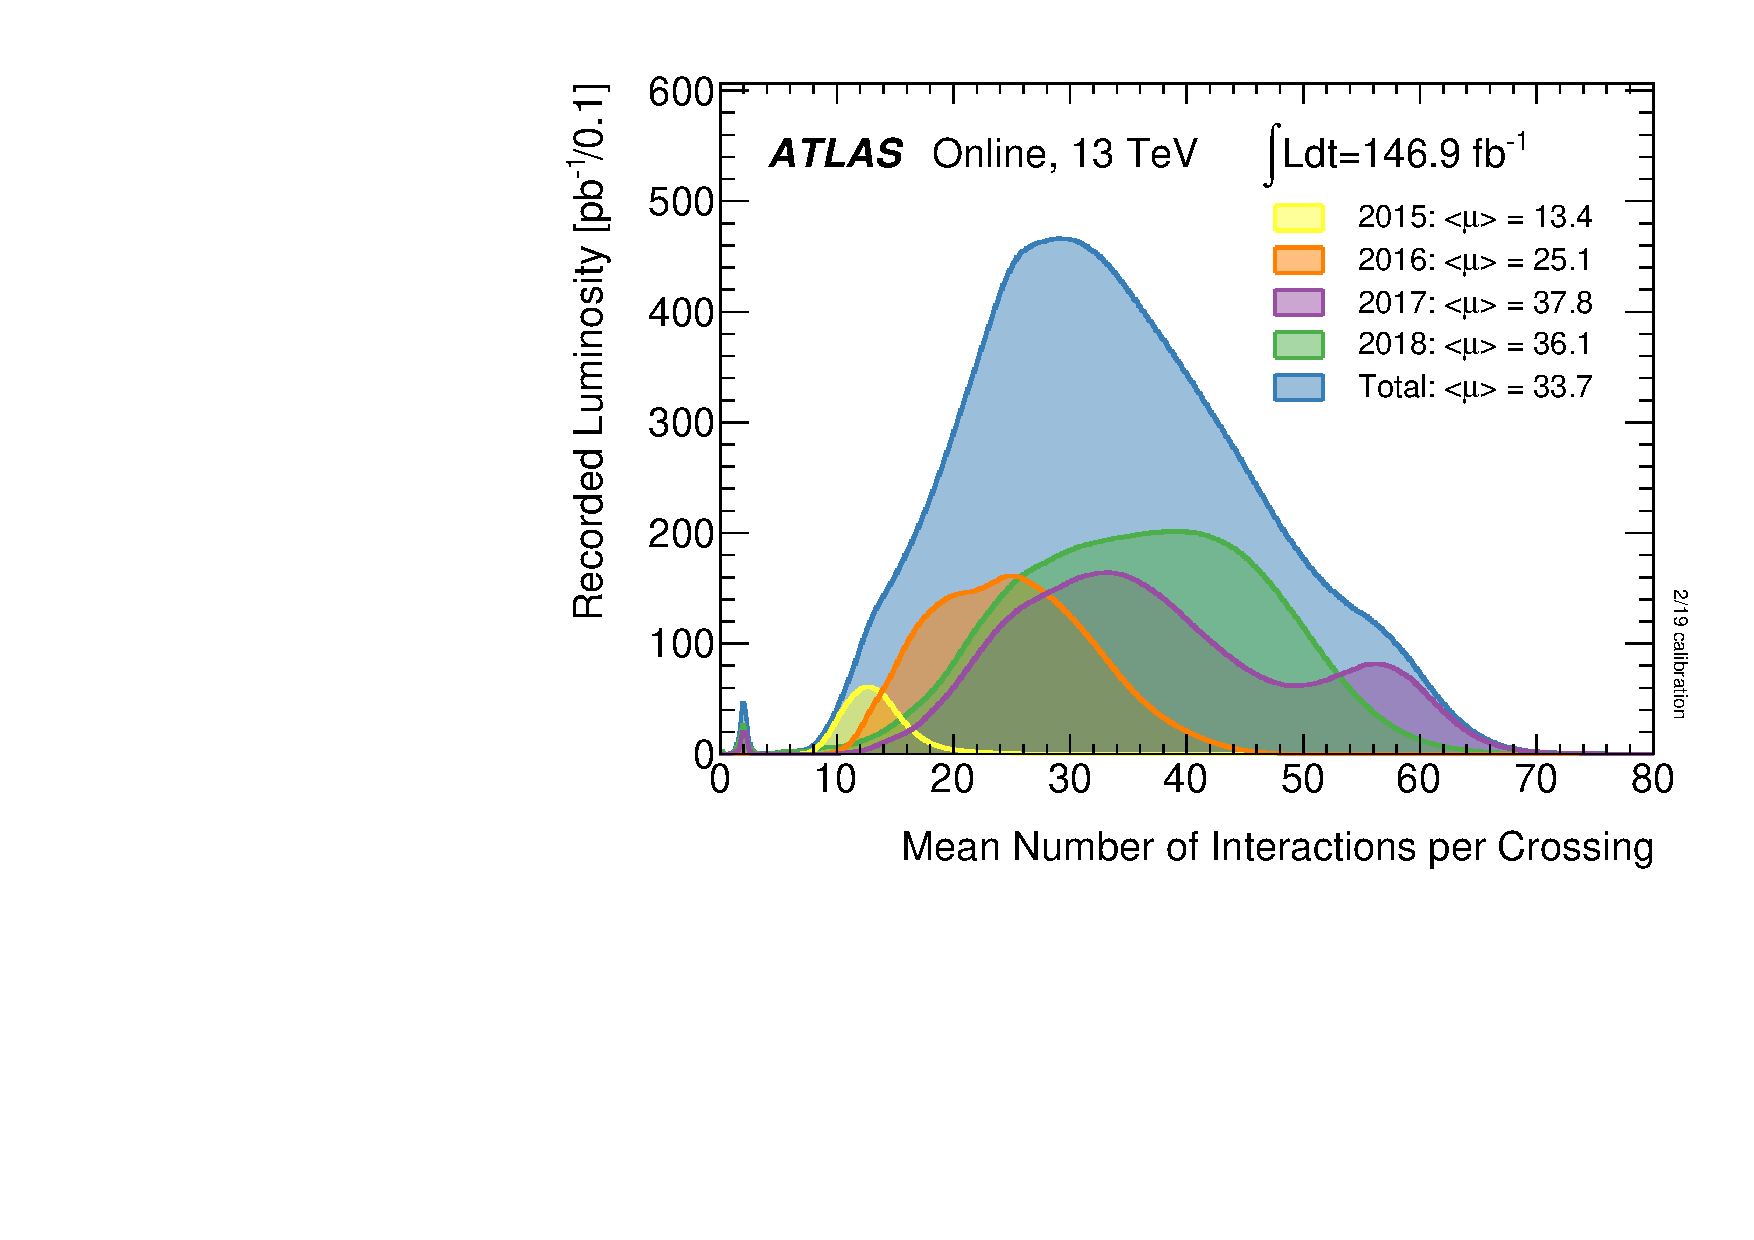
\includegraphics[width=0.5\textwidth]{mu_2015_2018}
    \caption[]{Pile up profiles for run 2 data taking periods \citep{pileup}.}
    \label{fig:pileup}
\end{figure}

\subsubsection*{Small-R Jets}
At a first step contributions from pileup are reduced by subtracting the median transverse momentum density $\rho=\pt / A$ of jets found within $\eta<2.0$ multiplied by the active area of the jet $A_T$ as defined in \textsc{FastJet} \citep{cacciari2012fastjet}. Another reduction observes that the pileup corrected \pt is a function of the number of primary Vertices $N_\text{PV}$ and the mean number of interactions $\mu$ so that the pile up corrected transverse momentum reads
\begin{equation}
  \pt^\text{corr}=\pt-\rho A_T -\alpha(N_\text{PV}-1)-\beta\mu
\end{equation}
with parameters $\alpha$ and $\beta$. The effect of the correction is shown in figure \ref{fig:jet_pt_correction}.
\begin{figure}
  \centering
  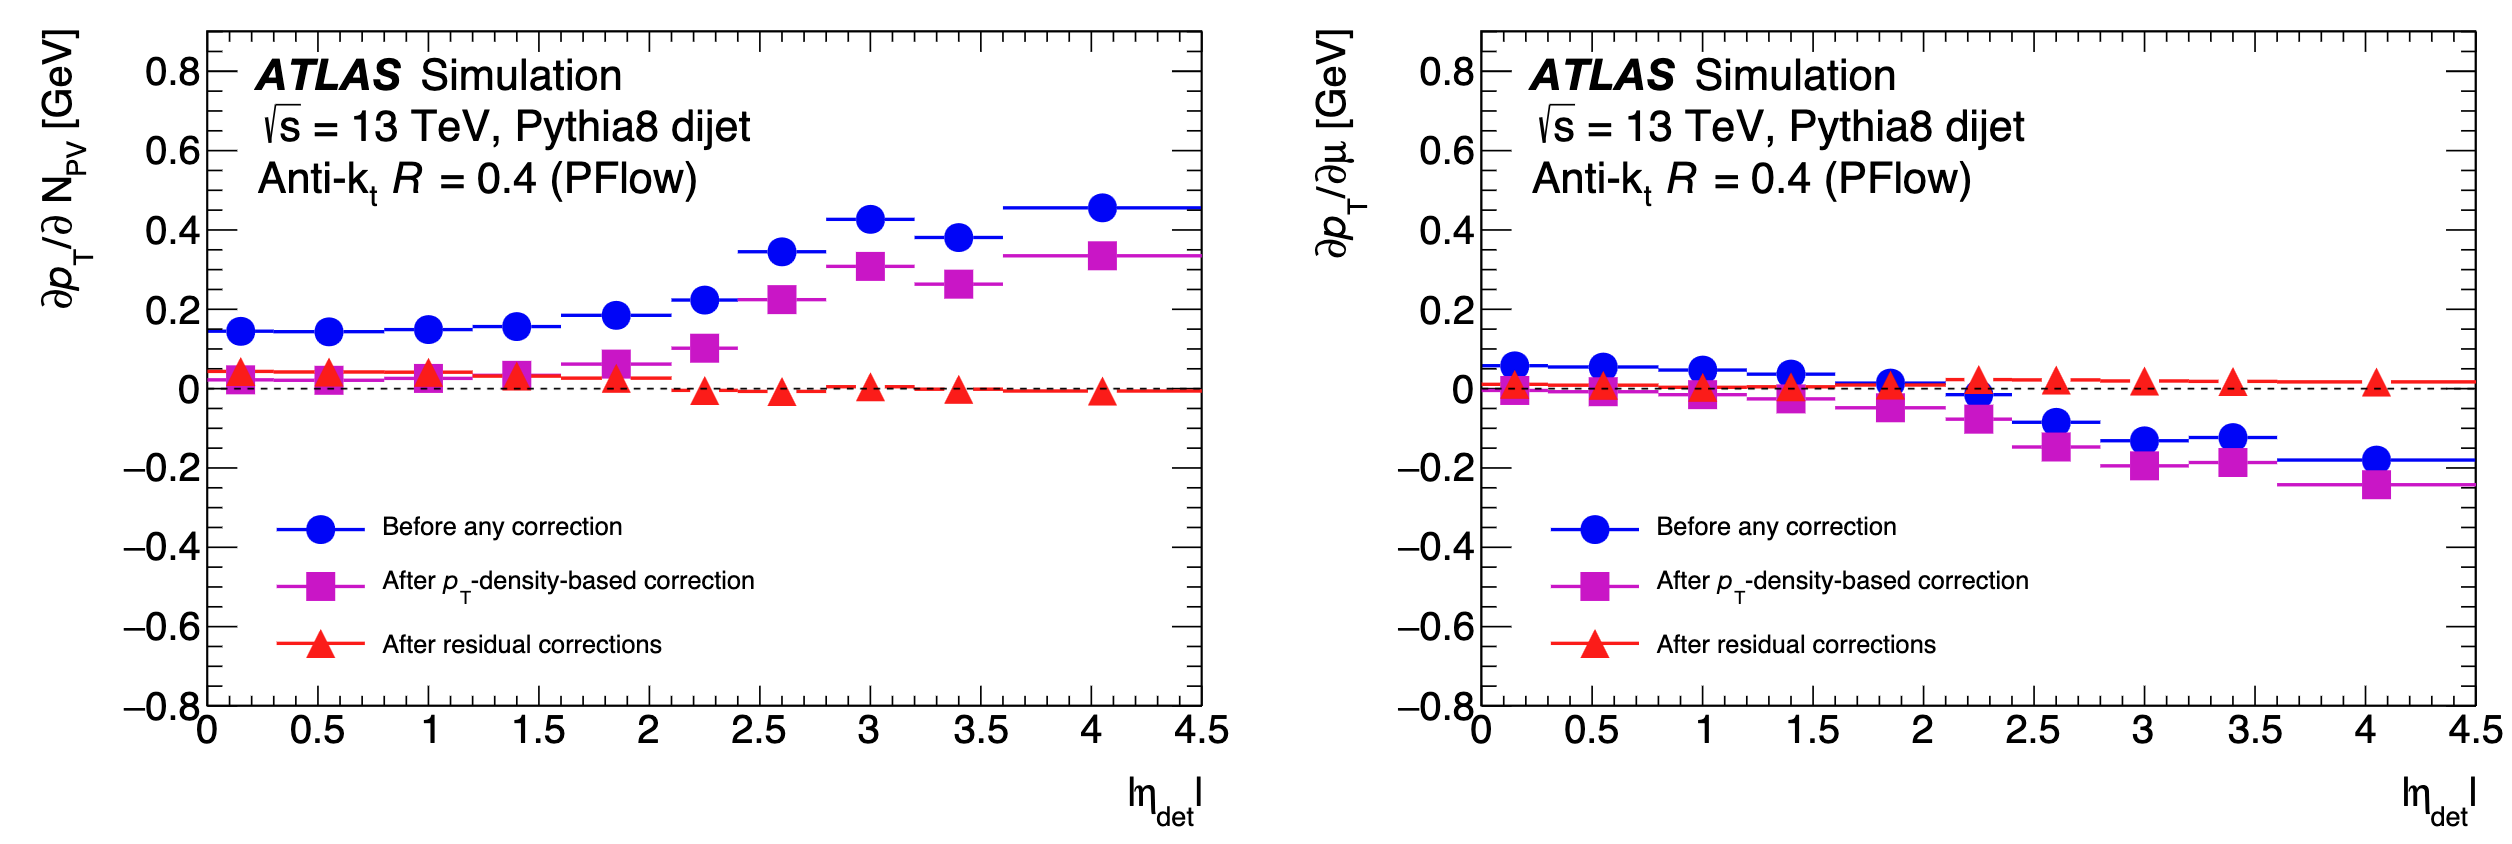
\includegraphics[width=1\textwidth]{jet_pt_correction}
  \caption[]{\pt correction to remove the \pt dependence of the jet at different $\eta$ for the \pt dependent on (left) the number of primary vertices and (right) average number of interactions of the collision.}
  \label{fig:jet_pt_correction}
\end{figure}

Moreover pileup contributions can be further reduced by comparing the scalar \pt sum of tracks from the \ac{pv} associated to the jet with the scalar \pt sum of all tracks including other \acp{pv}. The \ac{jvt} \citep{ATLAS-CONF-2014-018} utilizes this property to apply a quality criterion on jets with $\pt<\qty[]{60}{GeV}$ and $|\eta|<2.4$.


\subsubsection*{Large-R Jets}
Due to the large Area of large-R jets they are particularly susceptible to pileup contributions and therefore a technique called groomming is applied. For this a large R jet is reclustered into $R=0.2$ subjets for which only the ones are kept that have at least $\pt>\qty[]{5}{\percent}$ of the original large R jet \pt.

\subsection{\ac{jes}, $\eta$ and mass}
\begin{figure}
  \centering
  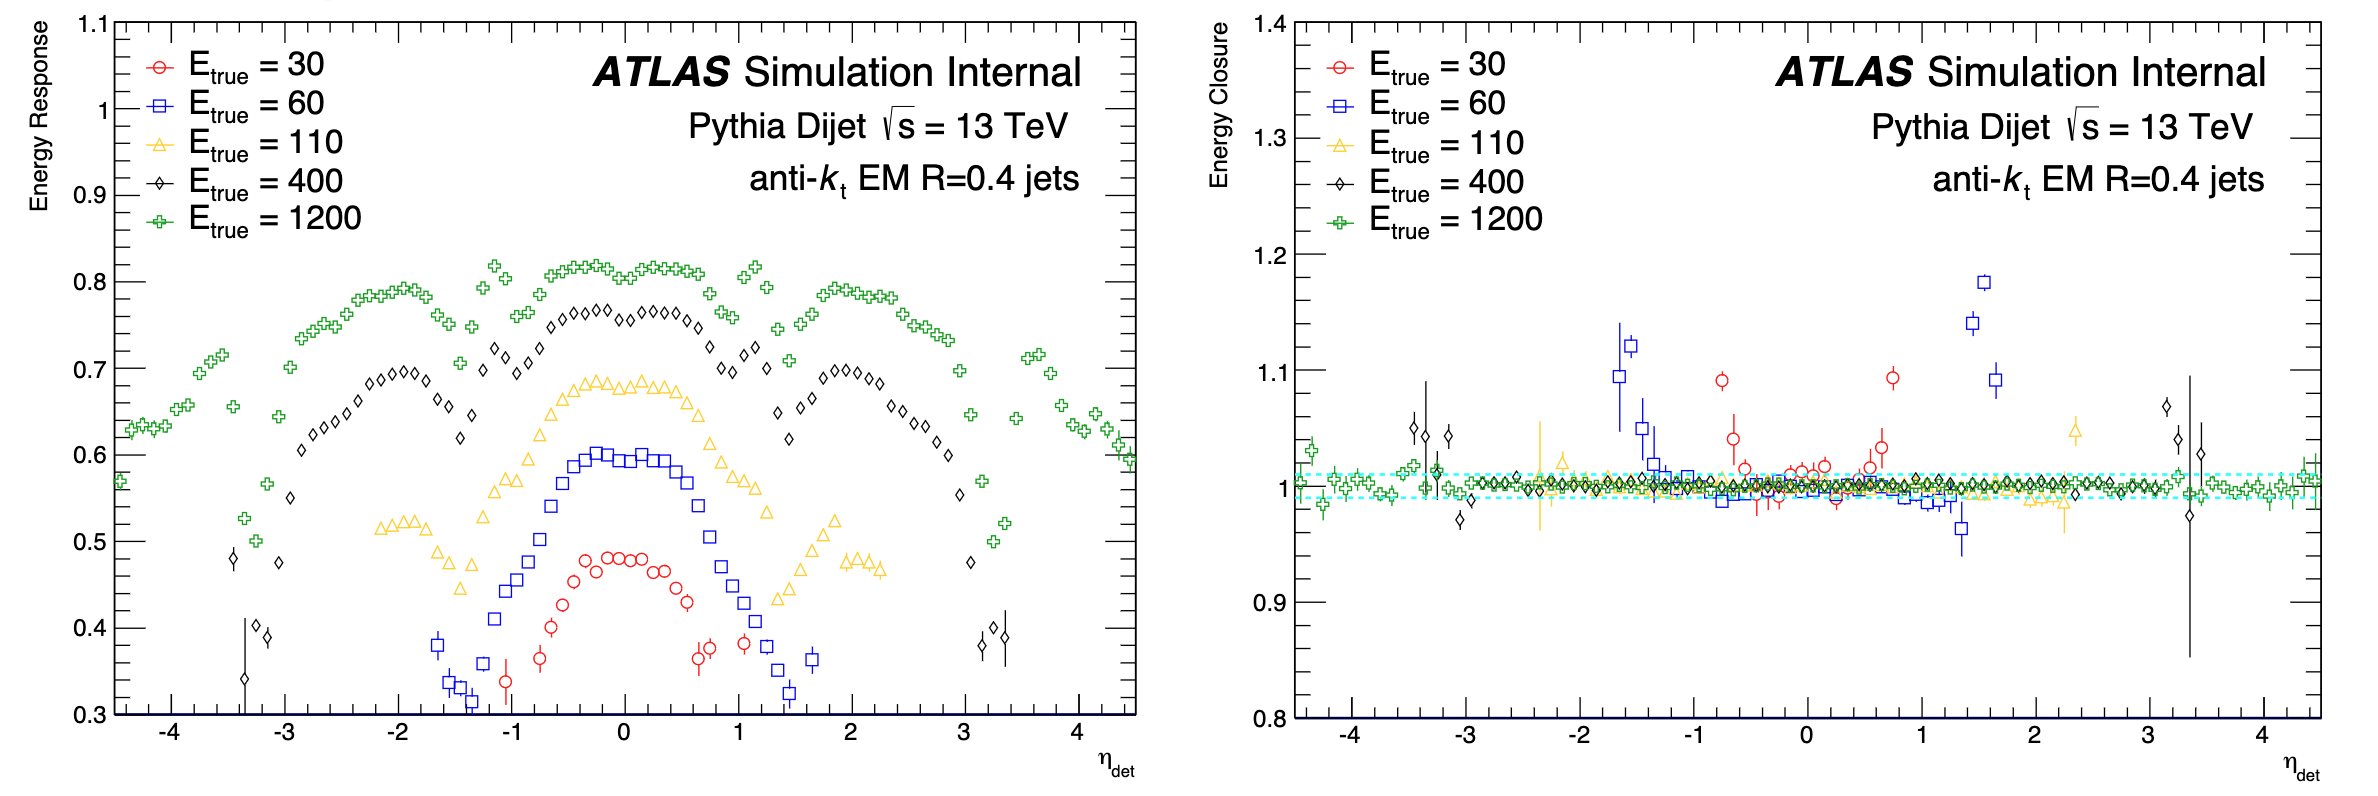
\includegraphics[width=1\textwidth]{jet_eta_mismatch}
  \caption[]{Jet energy response $E_\text{reco}/E_\text{truth}$ for different detector $\eta$ values (left) before and after applying (right) the calibration. Adopted from \citep{jet_eta_calib}.}
  \label{fig:jet_eta_mismatch}
\end{figure}
A clear mismatch between reconstructed and \ac{mc} truth two jet events can be seen in the left plot of figure \ref{fig:jet_eta_mismatch} measured in $\eta$ bins. From this a continuous correction function in $\eta$ is derived and applied to correct for differences in jet energy, $\eta$ and mass. This is exemplified in the right hand plot of figure \ref{fig:jet_eta_mismatch}.

\subsection{Global Sequential Calibration}

This step mainly corrects the jet \pt without changing the mean energy of the jet. It corrects for non-compensation, dead material and leakage effects by using observables like the charged particle fraction, energy fractions in different calorimeter layers, track-related quantities and the muon activity behind the calorimeter. Corrections are again derived in \pt and $\eta$ and are applied sequentially.

\subsection{In situ calibration}
At the final step differences between data and simulation are corrected for in \pt. These variations stem from imperfect simulations of detector materials and the modeling of the involved physics processes. For this well known physics processes are used and correction factors are extracted in \pt. This step is only applied to data.

\subsection{Mass correction for Large-R jets}
The mass of a jet is calculated from the energy deposits in calorimeter clusters $i$ and their transverse momentum as
\begin{equation}
  m_{\text{calo}} = \sqrt{\left(\sum_{i\in \text{Jet}}E_i\right)^2-\left(\sum_{i\in \text{Jet}}\vec{p_i}\right)^2}.
\end{equation}
The spread of decay products inside large-R jets scales with $1/\pt$. For very boosted jets the spread can become the size of the granularity of the calorimeter and the energy resolution degrades. With the help of tracking information the energy and mass resolution can be improved across the whole \pt range \citep{Aaboud:2019aa}. The track assisted jet mass is then
\begin{equation}
  m_{\text{TA}} = \frac{p_{\text{T}}^{\text{calo}}}{p_{\text{T}}^{\text{track}}} \cdot m_{\text{track}}
\end{equation}
where $p_{\text{T}}^{\text{calo}}$ is the transverse momentum measured in the calorimeter, $p_{\text{T}}^{\text{track}}$ is the transverse momentum of the four-vector sum of tracks associated to the large-R jet and $m_\text{track}$ is the invariant mass of this four-vector sum of tracks. Since the \ac{id} is only susceptible to charged particles the ratio of $p_{\text{T}}^{\text{calo}}$ and $p_{\text{T}}^{\text{track}}$ scales the mass measured from tracks to include neutral particles. The improvement is visualized in figure \ref{fig:combined_mass_large_R}. The calorimeter and track-assisted mass measurement are then linearly combined with a weight $w$ to give optimal results
\begin{equation}
  m_{\text{comb}} =  w\cdot m_{\text{calo}}+(1-w)\cdot m_{\text{TA}}.
\end{equation}
\begin{figure}
  \centering
  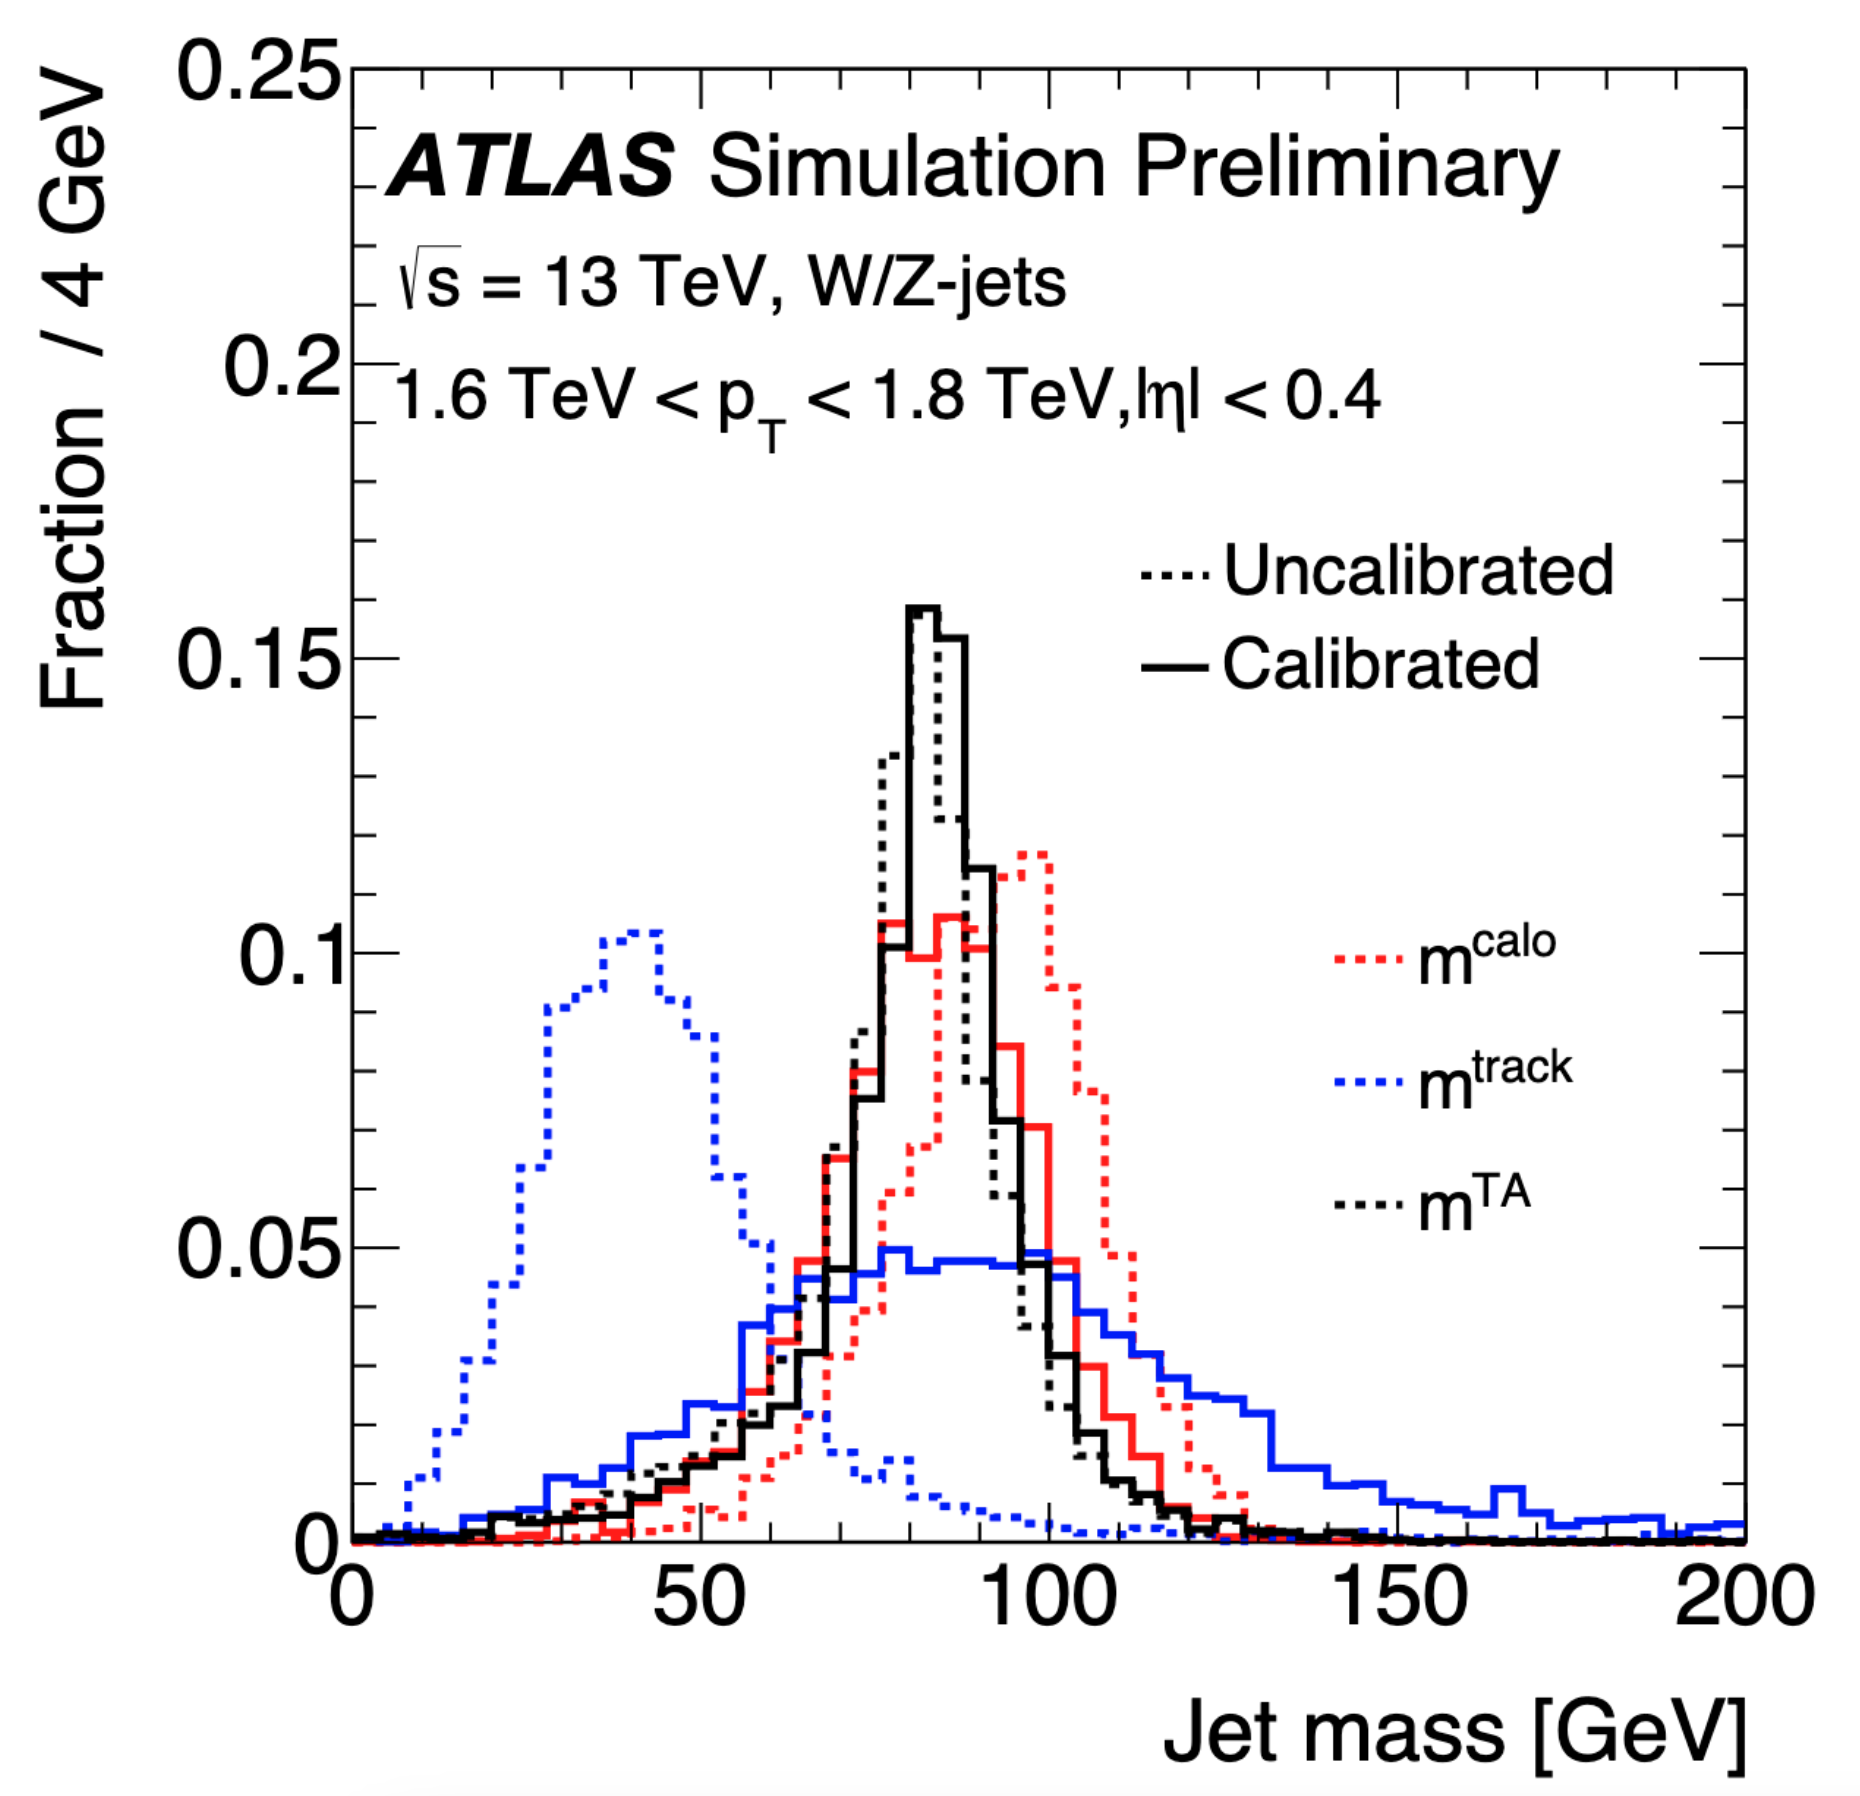
\includegraphics[width=.5\textwidth]{combined_mass_large_R}
  \caption[]{Improvement for track-assisted mass measurement compared to calorimeter and tracking information only. Adopted from \citep{ATLAS-CONF-2016-035} }
  \label{fig:combined_mass_large_R}
\end{figure}

% \chapter{The HH$\rightarrow$4b analysis}

The search for the exact shape of the Higgs potential is an interesting endeavor as its not only  directly related to \ac{ewsb} but also could solve some fundamental questions about the nature of the universe as described in section \ref{sec:beyond_sm}. Since the Higgs interacts via Yukawa couplings from equation \ref{eq:yukawa_term} the coupling strengths for fermions are directly proportional to their mass and thus the Higgs couples most strongly to heavy particles. The main production modes at the \ac{lhc} are shown in figure \ref{fig:main_production_processes}. All couplings in the following are scaled with respect to their \ac{sm} values and are denoted with $\kappa_\mathrm{c} = c/c_\mathrm{sm}$ so that $\kappa_\mathrm{c}=1$ represents the \ac{sm} value of some coupling $c$.

The dominant Higgs pair production processes are shown in figure \ref{fig:main_production_processes}. The first two \ac{ggf} diagrams (a) and (b) have a cross-section of
$\sigma_\text{vbf HH}^\text{SM}=\qty[]{31.05}{fb}$ calculated at a center of mass energy of \qty[]{13}{TeV} at \ac{nnlo} \citep{Grazzini_2018} while the \ac{vbf} processes (c), (d) and (e) of figure \ref{fig:main_production_processes} have a production cross-section of
$\sigma_\text{vbf HH}^\text{SM}=\qty[]{1.73}{fb}$ at \ac{nnnlo} \citep{PhysRevD.98.114016}. A characteristic of the \ac{vbf} processes is that the Higgs pair products are accompanied by two additional quarks. The \ac{vbf} cross section is about \qty[]{3e4}{} times smaller than the production cross section for single Higgs $\sigma_\text{H}^\text{SM}=\qty[]{48.58}{pb}$ at the \ac{lhc} \citep{de2016arxiv} which already illustrates the challenge of discovering Higgs pairs in these final states.
\begin{figure}
    \centering
    \subfigure[]{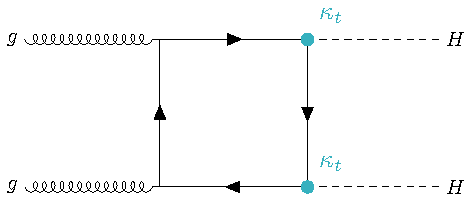
\includegraphics[width=.43\textwidth]{fig_01a}}\hspace{.06\textwidth}
    \subfigure[]{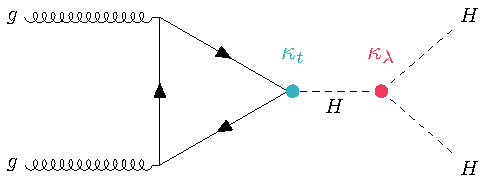
\includegraphics[width=.43\textwidth]{fig_01b}} \\
    \subfigure[]{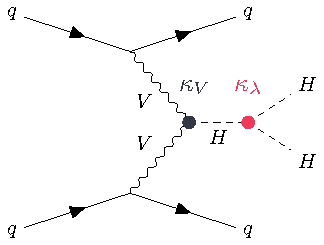
\includegraphics[width=.3\textwidth]{fig_02a}}\hspace{.01\textwidth}
    \subfigure[]{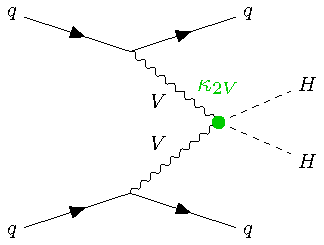
\includegraphics[width=.3\textwidth]{fig_02b}}\hspace{.01\textwidth}
    \subfigure[]{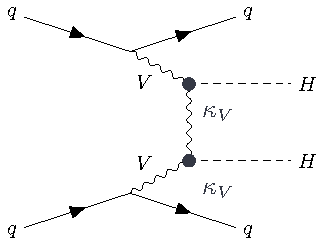
\includegraphics[width=.3\textwidth]{fig_02c}}
    \caption[]{Leading Higgs Pair production processes at the \ac{lhc}. (a), (b) shows \ac{ggf} and (c), (d), (e) \ac{vbf} processes. Adopted from \citep{aad2023search}.}
    \label{fig:main_production_processes}
\end{figure}
% higgs hat keine Ladung whatsoever cannot couple em or qcd 

\begin{figure}
    \centering
    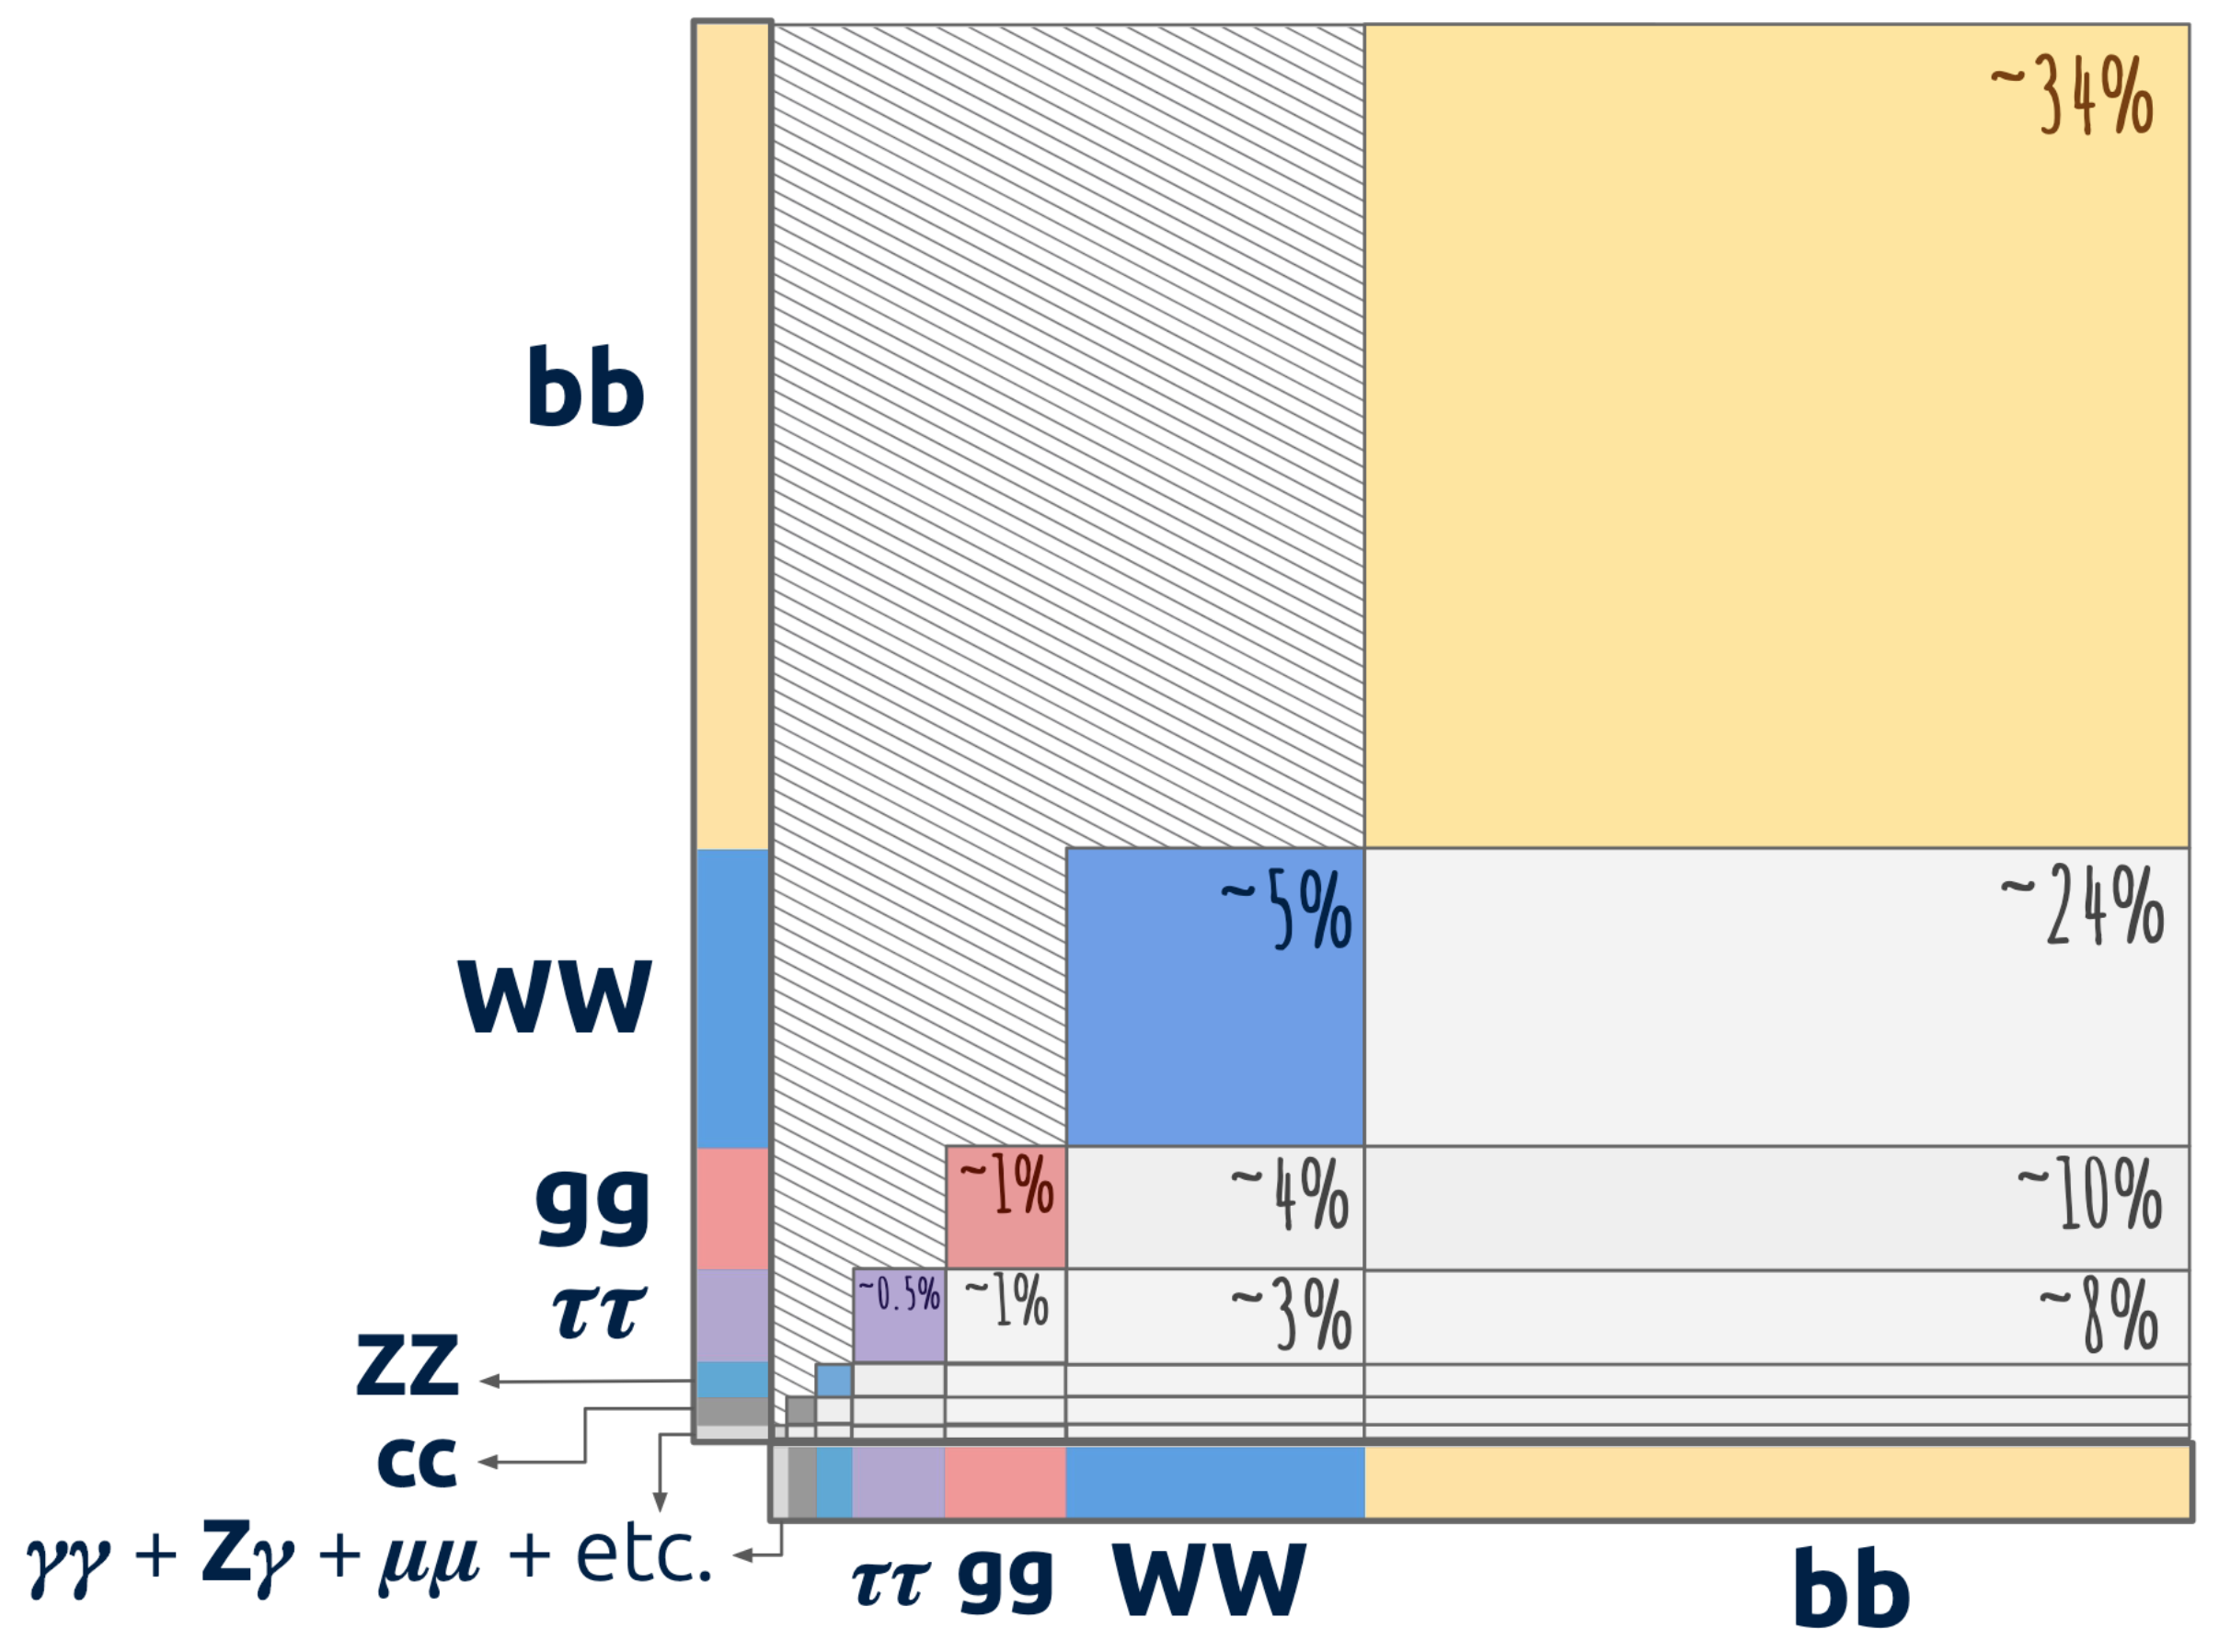
\includegraphics[width=0.7\textwidth]{branching_fraction_hh}
    \caption[]{Contributions of final states represented by area for a pair of Higgs \citep{Abbott:2708599}}
    \label{fig:branching_fraction_hh}
\end{figure}
Figure \ref{fig:branching_fraction_hh} reveals that an interesting channel is the final state with the largest branching fraction of about \qty[]{34}{percent} consisting of four $b$-quarks. However as this a fully hadronic final state it comes with the challenge of large \ac{qcd} backgrounds.

This work focuses on the boosted topology of highly energetic jets which do not allow reconstruction of $b$-jets individually but rather of final states consisting of two collimated $b$-jets inside a larger jet. The advantage of this selection is that it reduces greatly the \ac{qcd} backgrounds since highly energetic jets aare more likely to come from heavy particles such as $b$ quarks. Furthermore it is easy to trigger on events containing jets with large \pt. Although they represent a comparatively clean signal such events are rare and therefore have limited statistical power. For this reason other search strategies are better suited for the discovery of the Higgs pair production process.

A reason for the low cross-section is that diagrams (d) and (e) of figure \ref{fig:main_production_processes} cancel each other destructively for \ac{sm} values. In turn if $\ktwov$ is moved to non-\ac{sm} values the production cross-section increases significantly $\sigma_{\ktwov=0}\approx 20\sigma_{\ktwov=1}$ \citep{bishara2017higgs} and the decay products have much larger transverse momentum as shown in figure \ref{fig:kappa_2v_variations_mhh}.
\begin{figure}
    \centering
    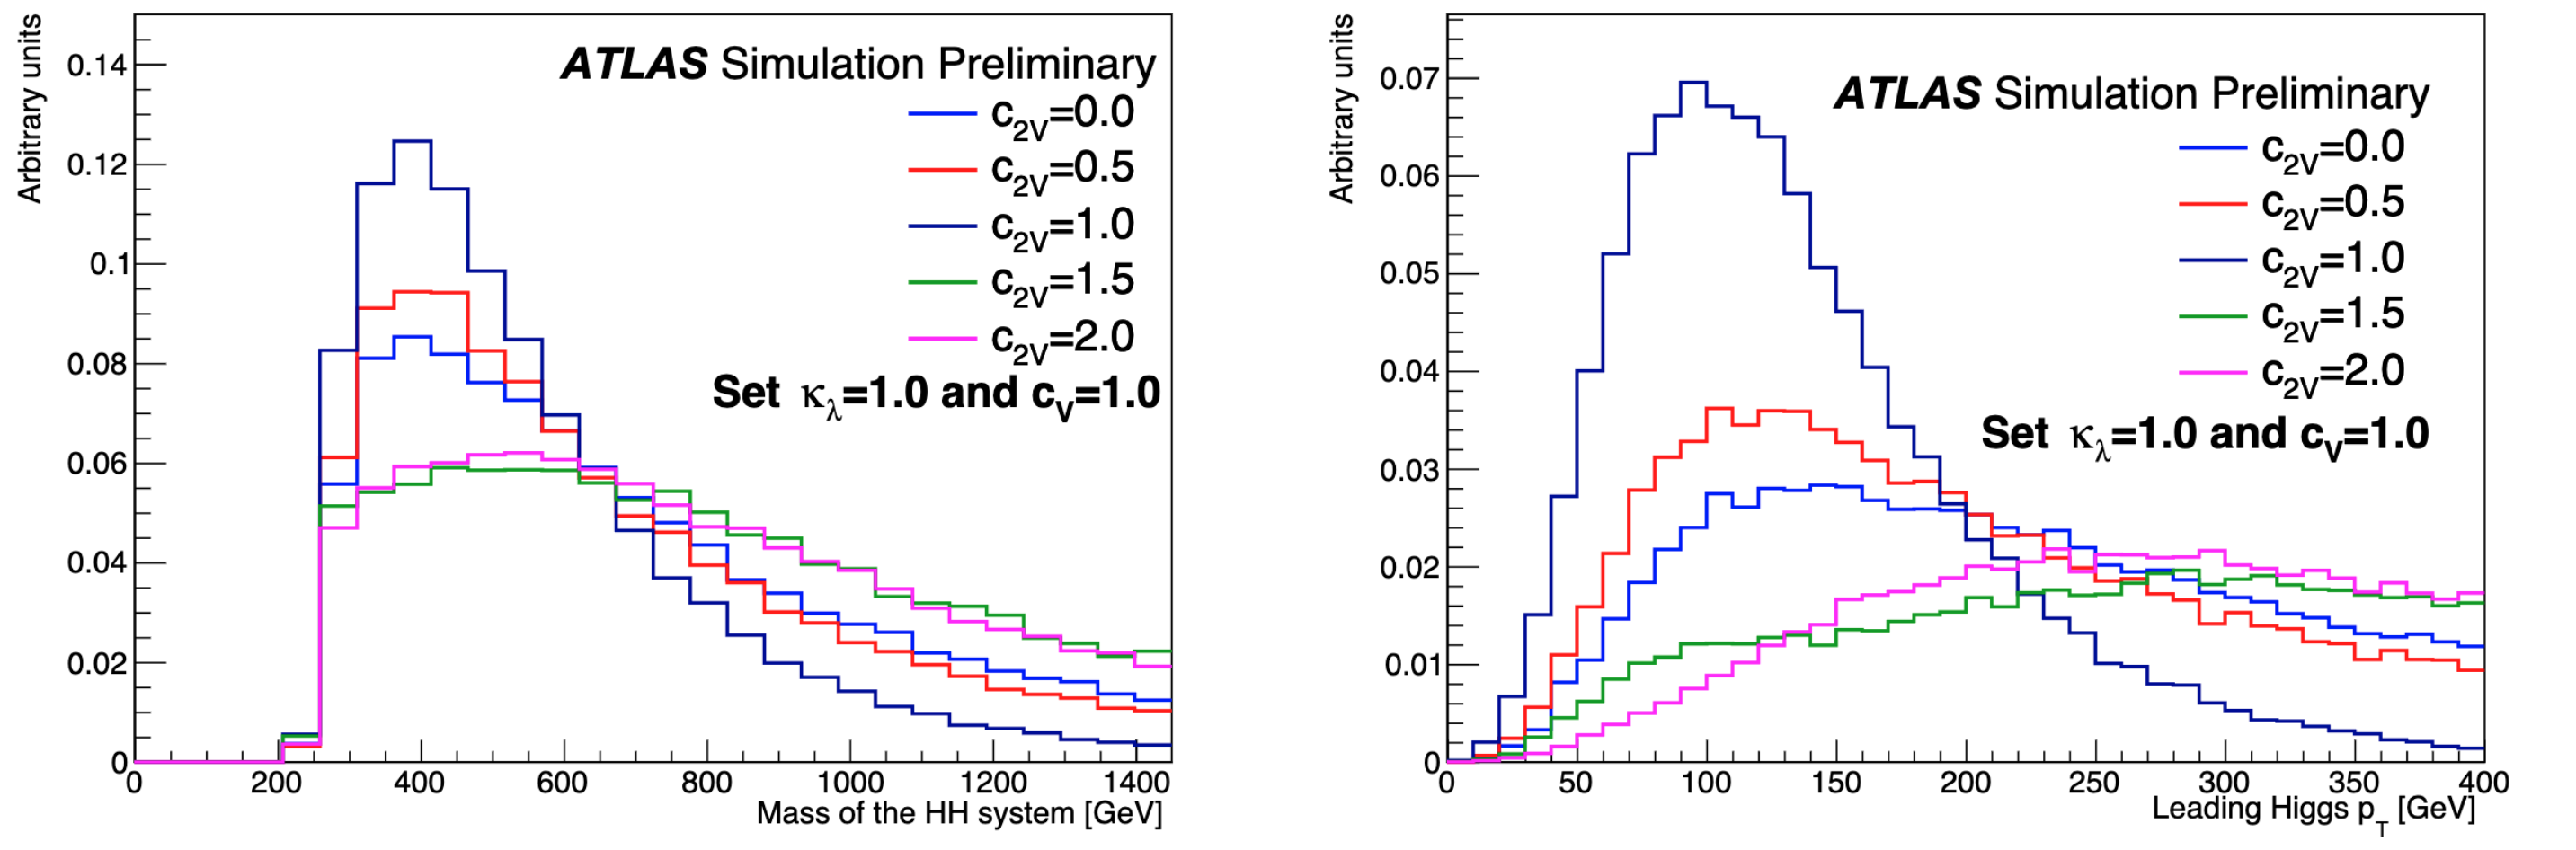
\includegraphics[width=1\textwidth]{kappa_2v_variations_mhh}
    \caption[]{Invariant mass of the Higgs pair system and the leading Higgs candidate jet \pt  reconstructed from simulation for different \ktwov. Adopted from \citep{ATL-PHYS-PUB-2019-007}.}
    \label{fig:kappa_2v_variations_mhh}
\end{figure}
Because of this behavior the power of this analysis lies in constraining and proving the existence of the \ktwov couplings within the \ac{sm} to which it is directly sensitive.



\section{Data and Monte Carlo Simulation}
This analysis uses the full run 2 data taken by \ac{atlas} between 2015 and 2018. The dataset contains \qty[]{140.1}{fb^{-1}} of data good for physics at a center of mass energy of \qty[]{13}{TeV} \citep{DAPR-2021-01}.

\ac{mc} generation in \ac{atlas} is done in three steps. At first at parton level events are generated with \textsc{MadGraph} (v.2.7.3p3.atlas6) \citep{alwall2014automated}. The output of this tool are stochastically sampled four vectors of the final states of the process of interest.

Afterwards \textsc{Pythia8} \citep{Sjostrand:2014zea} simulates the hadronization process. Because of the scaling behavior of \ac{qcd} described in \ref{sec:renormalization} partons inside a proton cannot be modeled since the perturbation ansatz of \ref{sec:qft} breaks down. However the partons momentum fraction can be deduced from \acp{pdf} by measuring them at some energy scale. For this the \textsc{NNPDF3.0nlo} \ac{pdf} is used by \textsc{Pythia8}. For normalization the \ac{sm} \ac{vbf} cross-section is multiplied by the 4b branching ratio $\mathcal{B}(4b)=0.3392$.


\red{add samples linear combination}
% https://www.overleaf.com/project/638e1930f926cd21d5264259
% linear combination
% Unfortunately, MC generation is computationally expensive and time-consuming. As such, only1443
% a handful of MC simulation samples for only a handful of coupling values are actually produced, and a1444
% sample combination technique is employed to model the signal hypothesis across the coupling parameter1445
% space
% https://trexfitter-docs.web.cern.ch/trexfitter-docs/model_building/expression/
% https://gitlab.cern.ch/hh4b/hh4b-boosted-vbf-limits/-/blob/main/create_workspaces/configs/k2V_parameterized_BDT_decorXbb.config?ref_type=heads#L285-331

\section{Analysis objects}
This section presents the details of the reconstruction for the objects used in the analysis. 
\subsection{Large Radius Jets}
Large 
\subsection{$X\rightarrow bb$ tagger}

% This work focuses on the boosted regime of the 4 $b$-quark final state. If jets are very boosted two $b$-jets can overlap and are reconstruct as variable radius jets inside a larger jet.
% as explained in section \ref{sec:vr_jets}.

% xbb tagger citation
% \citep{ATL-PHYS-PUB-2020-019}
% https://cds.cern.ch/record/2724739/files/ATL-PHYS-PUB-2020-019.pdf
% https://cds.cern.ch/record/2777811/files/ATL-PHYS-PUB-2021-035.pdf
% https://cds.cern.ch/record/2866601/files/ATL-PHYS-PUB-2023-021.pdf
% modeling

\subsection{Small Radius Jets}
\section{Analysis Strategy}
To fully capture the boosted topology of two jets that contain 2 collimated $b$-jets each so called Large R jets are used. These are formed with a radius parameter of $R=1.0$ for the Anti-$k_t$ clustering algorithm described in \ref{sec:anti_kt}.

region definitions
\subsection{Trigger}
\subsection{Event selection}
\subsubsection{Kinematic Selection}
\subsection{Background Estimation}


% \chapter{Analysis Optimization}\label{sec:analysis_optimization}
After carefully designing physical objects to represent the final state of a physical process of interest the main task is to construct a quantity that tests the compatibility of the prediction with the observation. Typically this is a kinematic variable such as the invariant mass of the Higgs pair system $m_\text{HH}$ in this analysis, designed to differentiate signal from background. Since the statistical test is based on frequentist statistics as further explained in chapter \ref{sec:statistics} a histogram is constructed from the final quantity. Usually at each step leading to this quantity it is optimized on some ratio of signal to background.

Since the purpose of this quantity is to optimally separate signal from background it is actually better suited to be treated with a \ac{ml} model as already applied widely in particles physics \citep{albertsson2019machine,shlomi2020graph,feickert2021living,Schwartz2021Modern}. These models are typically trained to categorize input events into signal and background(s). However a key issue with signal to background optimization is that they are not optimized for the actual final quantity of interest like a discovery significance or the level of confidence if a tested hypothesis should be accepted or rejected.

While the signal-to-background ratio or the separation ability of the \ac{ml} model may correlate to some extent with the expressivity of the statistical test, it is not optimal, particularly because it does not account for uncertainties that can significantly impact the outcome of the statistical test. This means that even if the statistical test performs exceptionally well on nominal values, its effectiveness may dramatically diminish when presented with inputs that deviate from these nominal values due to uncertainties.

This issue can be addressed with: \textit{\ac{neos}} \citep{Simpson_2023}. It is based on the observation that the classifier training can be done with respect to the actual final quantity of interest by integrating the statistical model into the training.


\section{Machine Learning}
\ac{ml} refers to algorithms that enable computers to learn from data to make predictions for some specific task without being explicitly programmed for \citep{kubat2021introduction}. One particular subset of \ac{ml} are \acp{ann} inspired by the human brain. Their fundamental unit are nodes, the neurons, that are interconnected to several other neurons organized in consecutive layers with an initial input and a desired output as shown in figure \ref{fig:ann}. The signals between neurons are transferred weighted and each neuron has an activation function that converts the received input stimulus into an output strength. Thus learning occurs through adjusting the weights between the neurons. \acp{ann} can be designed in various ways with many layers depending on the specific task.
\begin{figure}
    \centering
    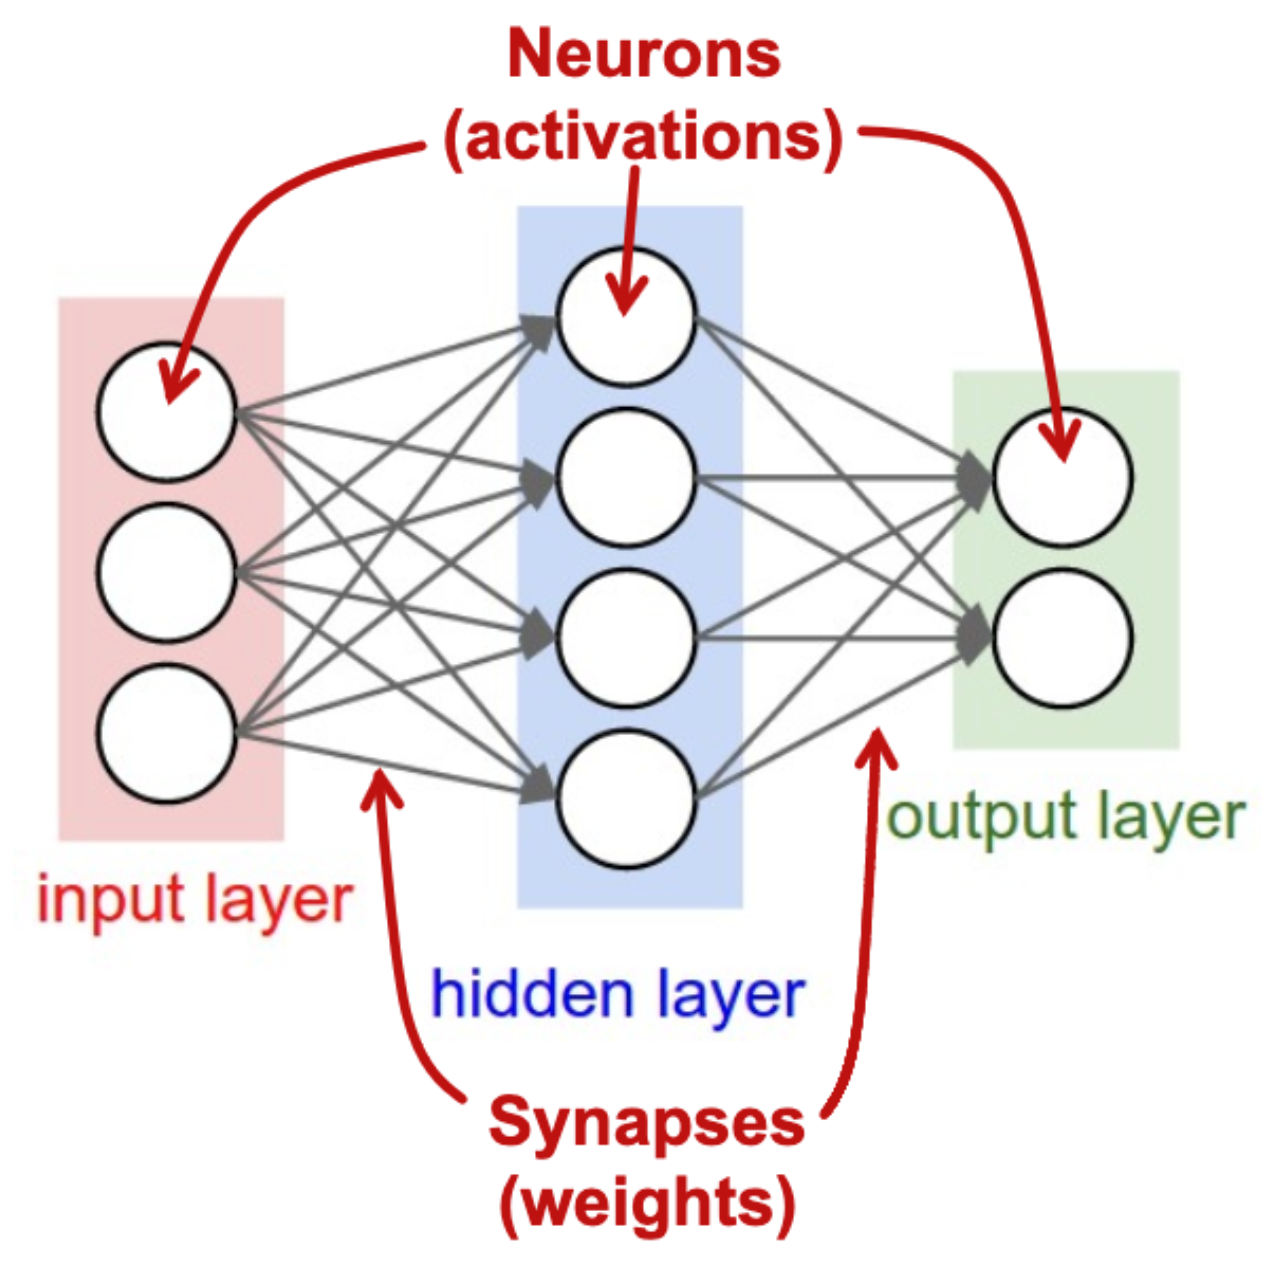
\includegraphics[width=0.4\textwidth]{ann}
    \caption[]{Structure of artificial feed-forward neural networks. Adopted from \citep{8114708}.}
    \label{fig:ann}
\end{figure}

The training of \acp{nn} is usually done with the back-propagation algorithm which seeks to minimize a cost function $C(\bm{\varphi})$ that is designed to measure the deviance of a presented input to a desired output dependent on the model parameters $\bm{\varphi}$. For a feed-forward \ac{nn} these model parameters are the mentioned weights and added biases of the neurons. Via gradient descent the minimum of the cost function can be found stepwise with the first derivative and a chosen learning rate parameter $\gamma$
\begin{equation}
    \bm{\varphi}_{n+1} = \bm{\varphi}_n-\gamma\nabla C(\bm{\varphi}_n).
    \label{eq:grad_descent}
\end{equation}
In three dimensions this corresponds to a mountaineer searching for the valley by going in the direction of the steepest crescent with a stepsize proportional to $\gamma$.



\section{NEOS}
The key idea of \acl{neos} is to choose the cost function as the quantity which is to be minimized. In this case the $\mathrm{CL}_s$ value is a reasonable choice as discussed in chapter \ref{sec:statistics}. For a typical analysis chain as shown in figure \ref{fig:neos} this translates into a mathematical concatenation of the individual steps within the chain.
\begin{figure}
    \centering
    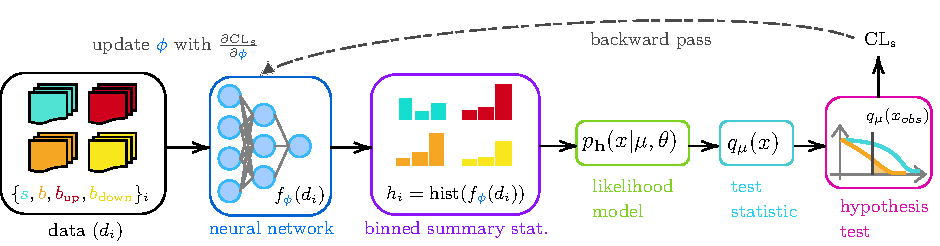
\includegraphics[width=1\textwidth]{neos}
    \caption[]{Typical particle physics analysis chain. For \ac{neos} the $\text{CL}_s$ value is back-propagated to train the neural network parameters $\bm{\varphi}$. Adopted from \citep{Simpson_2023}.}
    \label{fig:neos}
\end{figure}
Hence the cost function $\text{CL}_s$ is a function of the dataset $\mathcal{D}$ and the \ac{ml} model parameters $\bm{\varphi}$
\begin{equation}
    \mathrm{CL}_s = f(\mathcal{D},\bm{\varphi}) = (f_{\mathrm{sensitivity}} \circ f_{\mathrm{test\,stat}} \circ f_{\mathrm{likelihood}}  \circ f_{\mathrm{histogram}}  \circ f_{\mathrm{observable}})(\mathcal{D},\bm{\varphi}).
\end{equation}
In order to find the minimum via the gradient descent of equation \ref{eq:grad_descent} \cls needs to be differentiable with respect to $\bm{\varphi}$. By applying the chain rule this reads for one model parameter $\varphi_i$
\begin{equation}
    \frac{\partial\,\mathrm{CL}_s}{\partial \varphi_i} = \frac{\partial f_{\mathrm{sensitivity}}}{\partial f_{\mathrm{test\,stat}}}\frac{\partial f_{\mathrm{test\,stat}}}{\partial f_{ \mathrm{likelihood}}} \frac{\partial f_{\mathrm{likelihood}}}{\partial f_{\mathrm{histogram}}}   \frac{\partial f_{\mathrm{histogram}}}{\partial f_{\mathrm{observable}}}  \frac{\partial f_{\mathrm{observable}}}{\partial \varphi_i}.
\end{equation}
Apart from histogramming which is inherently discrete all other steps are differentiable. A method to render histograms differentiable is \ac{kde} \citep{CRANMER2001198}. Instead of counting a quantity in bins, a histogram can be approximated by representing each data point by a normal distribution termed the kernel. This distribution has the mean equal to the the data point's value and a chosen value for the standard deviation, also called the bandwidth in this context. Since the area under each Gaussian is equal to one, the collective addition of all Gaussian's yields a smoothed estimate of a histogram that is inherently differentiable. However, it is crucial to select the bandwidth appropriately, ideally around the desired bin width, as the quality of the KDE estimate is highly sensitive to this choice. This is demonstrated in Figure \ref{fig:relaxed_hist}. Although this can be a source of uncertainty any differentiable step or block in figure \ref{fig:neos} can always be reverted back to the exact calculation.
\begin{figure}
    \centering
    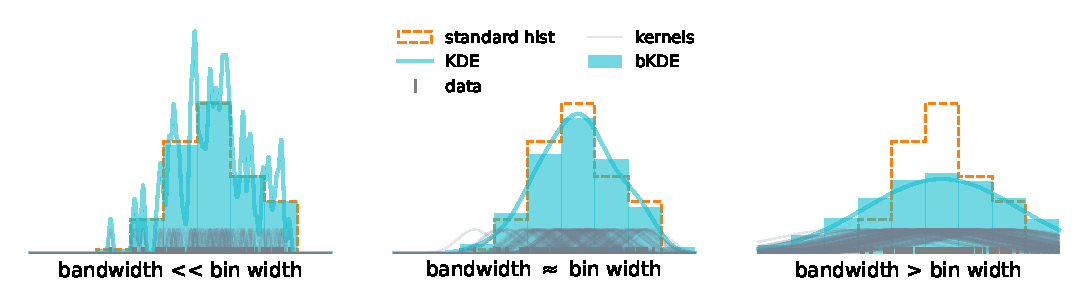
\includegraphics[width=1\textwidth]{relaxed_hist}
    \caption[]{Dependence of the histogram approximation with normal distributions of different standard deviations called bandwidth in the context of \ac{kde}. Depicted in grey small bars on the x-axis are the data points and in grey above them their kernel estimates. Further shown is the standard histogram binned from data, the \ac{kde} and the \ac{bkde} as a histogram calculated from the area under the \ac{kde} in a chosen bin range. Adopted from \citep{Simpson_2023}.}
    \label{fig:relaxed_hist}
\end{figure}


\subsection{Implementation}
Tracing differentiation through software is achievable by recognizing that any software essentially comprises a series of elementary arithmetic operations. Since the analytic solutions for these operations are known, the task reduces to concatenating all these operations and differentiating the resulting function. This is also known as \textit{Automatic Differentiation} and is achieved here with the help of the software package \textsc{jax} \citep{jax2018github}.

While the concept may appear straightforward, one of the challenges that previously hindered its implementation is the difficulty of differentiating across multiple individual software frameworks.That this became feasible within a reasonable time frame builds greatly on the transition efforts  of the individual steps to the \textsc{Python} programming language, moving away from C++ \textsc{ROOT}-based software \citep{ANTCHEVA20092499}. While \textsc{root} was indispensable at its time of emergence it is now less optimal for contemporary scientific analysis. This is because it is not only more difficult to integrate within other current software but also due to its user-unfriendliness compared to \textsc{Python} solutions which are maintained by a broad scientific community doing data-analysis. Using \textsc{python} in this context presents a notable advantage since as it benefits from widespread community support and pre-existing solutions to many common problems, enabling the use of tools like \textsc{jax}, which were not originally connected to \ac{hep}.


The original proposers \citet{Simpson_2023} of \ac{neos} developed differentiable versions of common \ac{hep} tasks like the upper mentioned hypothesis test, histogramming and the optimization of a cut in a packaged called \textsc{relaxed} \citep{Simpson_relaxed_version_0_3_0_2023}. They successfully tested the entire pipeline in a toy model \citep{Simpson_neos_version_0_2_0_2021}. These efforts were transferred and further developed to be applicable to this analysis with \citep{hh_neos}. \red{how about a better repo name: sensitivo, sensitivity optimizer, sensor, sensitor, sensoptimo}


% The text outlines systematic uncertainties in a physics analysis, distinguishing between Monte Carlo (MC) simulation uncertainties and those from data-driven backgrounds. MC uncertainties, per CP group recommendations, impact only the signal and are propagated accordingly. Luminosity uncertainty, at 0.83%, has minimal analysis impact. Jet-related uncertainties involve energy scale, resolution, and mass, corrected through established in situ methods and additional flavor/topology considerations. The \Xbb tagging efficiency discrepancy between data and MC is calibrated using $Z(\rightarrow \bb)+$ jets events, with overall stable calibration but some fluctuations at the 70% working point.

% The impact of \Xbb uncertainties is significant, affecting all signal events' BDT responses by about +70%/-50%. By de-correlating uncertainties across transverse momentum bins, the analysis's sensitivity is improved. Small-R jet uncertainties are calculated using the JetUncertainties tool, considering various effects like dijet balance and single-particle uncertainties.

% Theoretical uncertainties are considered for cross-section calculations and parton shower modeling. The latter compares \PYTHIA8 and \HERWIGV7 generated samples, applying an interpolation strategy for resonant signals. Reweighting uncertainties from ggF to VBF variations are deemed negligible after validation against simulation.

% Background uncertainties include normalization and shape variations. The normalization factor is derived from control regions with an uncertainty of 12.3% for non-resonant and 14.4% for resonant analyses. Shape uncertainties are estimated from validation regions, applying smoothing techniques like the 2-bin method to mitigate statistical fluctuations. Overall, the text concludes with a systematic summary table indicating the influence of each uncertainty on normalization and shape for both signal and background.
\chapter{Systematics Uncertainties}
Any measurement needs to consider uncertainties in order to determine its validity. In this analysis they can be divided into systematic errors for the reconstructed objects, uncertainties from theoretical calculations, methodological errors and statistical uncertainties and are described in the following

\section{Jet Uncertainties}
Jets are calibrated using well known reference objects as described in section \ref{sec:calibration}. These corrections are themselves subject to uncertainties related to detector effects, modeling and statistics leading to corrections of the jet energy and are collectively referred to as \ac{jes} \citep{atlas2021jet,Aaboud:2019aa}. Since simulations of jets have a higher accuracy than observed jets the uncertainties of the simulated jets are broadened to be consistent with the jets observed in the data. These uncertainties are known as \ac{jer}. Furthermore large-$R$ jets are additionally corrected for their mass. The uncer tainties related to this procedure are called \ac{jmr} \citep{ATLAS-CONF-2020-022}.

\section{$X\rightarrow bb$ Tagger Uncertainties}
The \ac{nn} of the $X\rightarrow bb$ tagger was trained using simulations leading to potential discrepancies in selection efficiencies between observed data and simulation. Calibration is conducted with $Z(\rightarrow b\overline{b})+$~jets and $Z(\rightarrow b\overline{b})+\gamma$ applying the same methodology as in \citep{ATL-PHYS-PUB-2021-035}. However as of this analysis the $b$-tagging algorithm for the \ac{vr} track jets has been updated to the DL1d algorithm described in section \ref{sec:b_tagging}. The differences between \ac{mc} and data are measured in large-$R$ jet \pt and the extracted scale factors and their corresponding combined systematic and statistical uncertainties are shown in figure \ref{fig:xbb_sf}.
\begin{figure} 
    \centering
        \subfigure[]{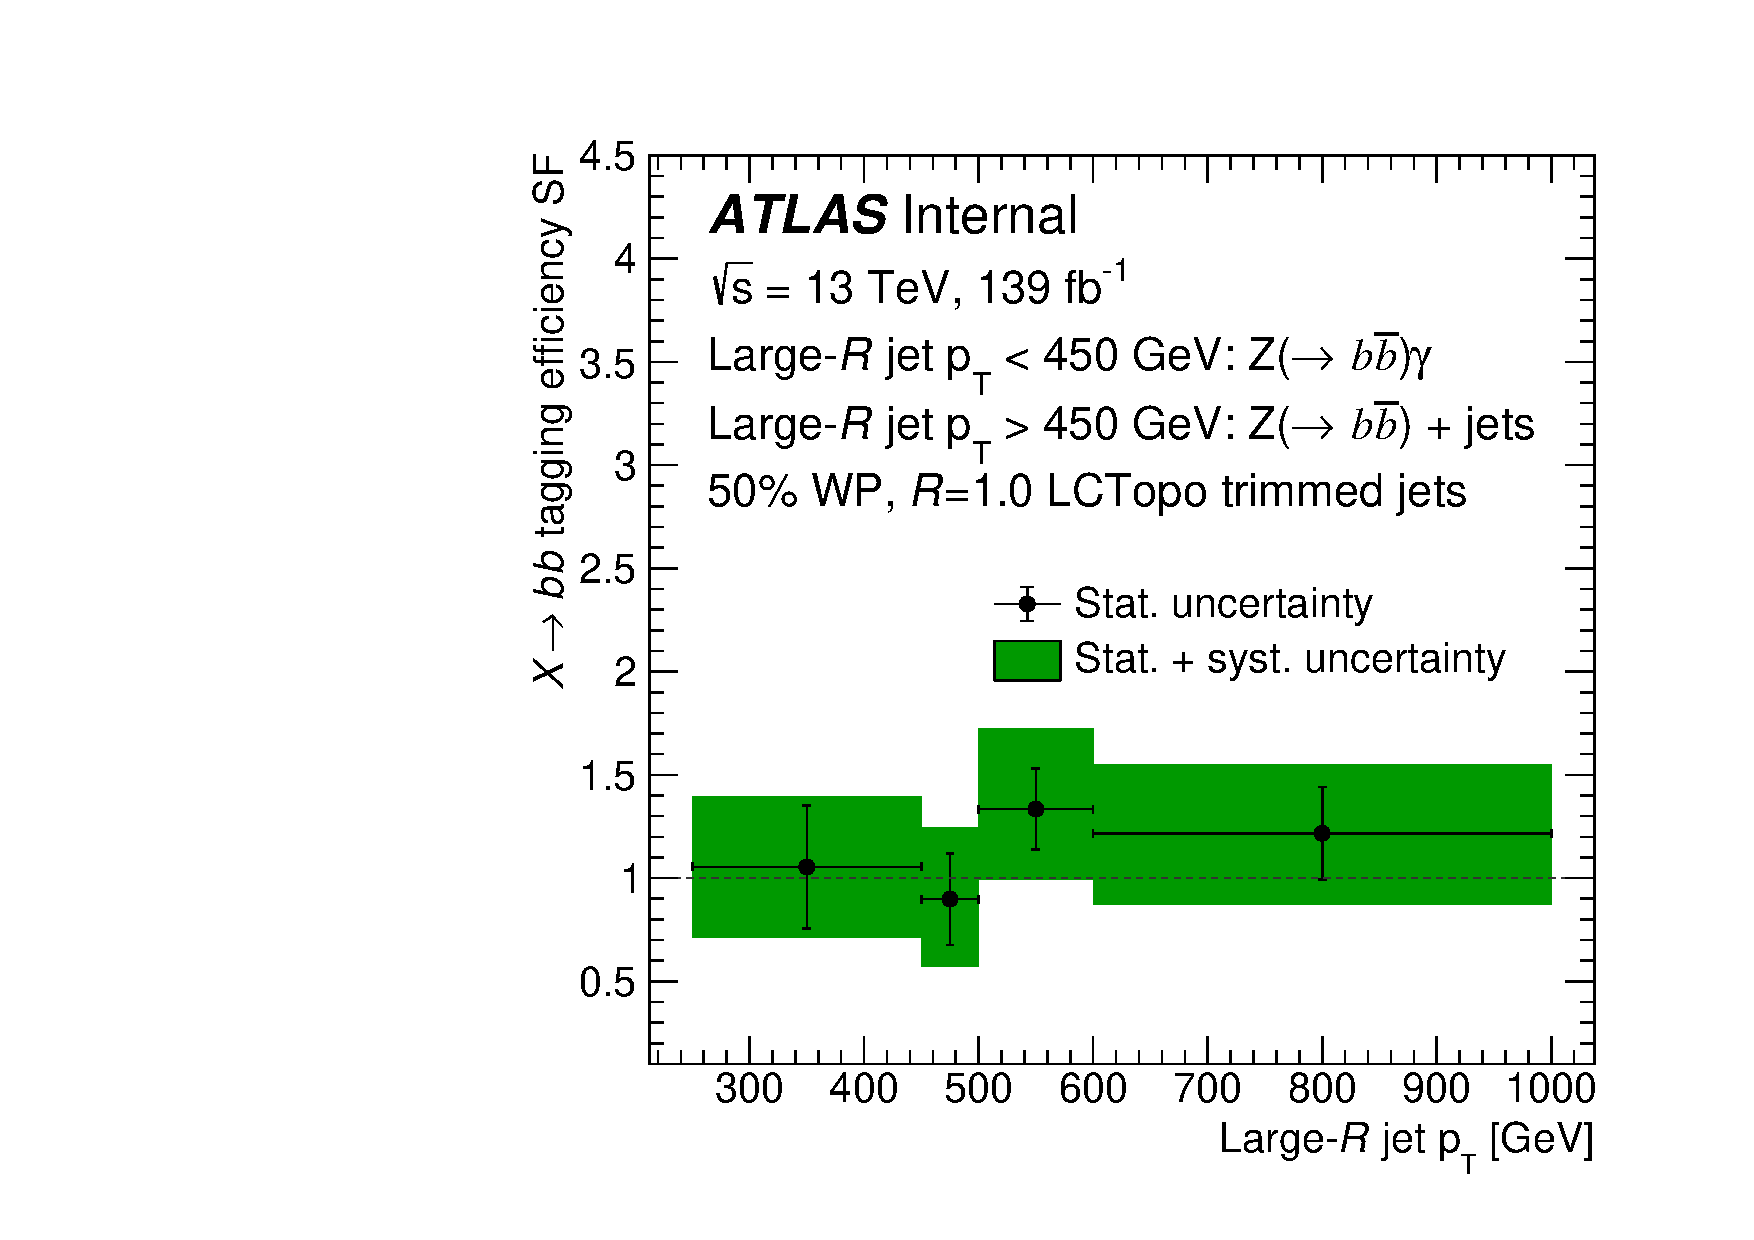
\includegraphics[width=.49\textwidth]{SF_Xbb50_internal_09March2023}}
        \subfigure[]{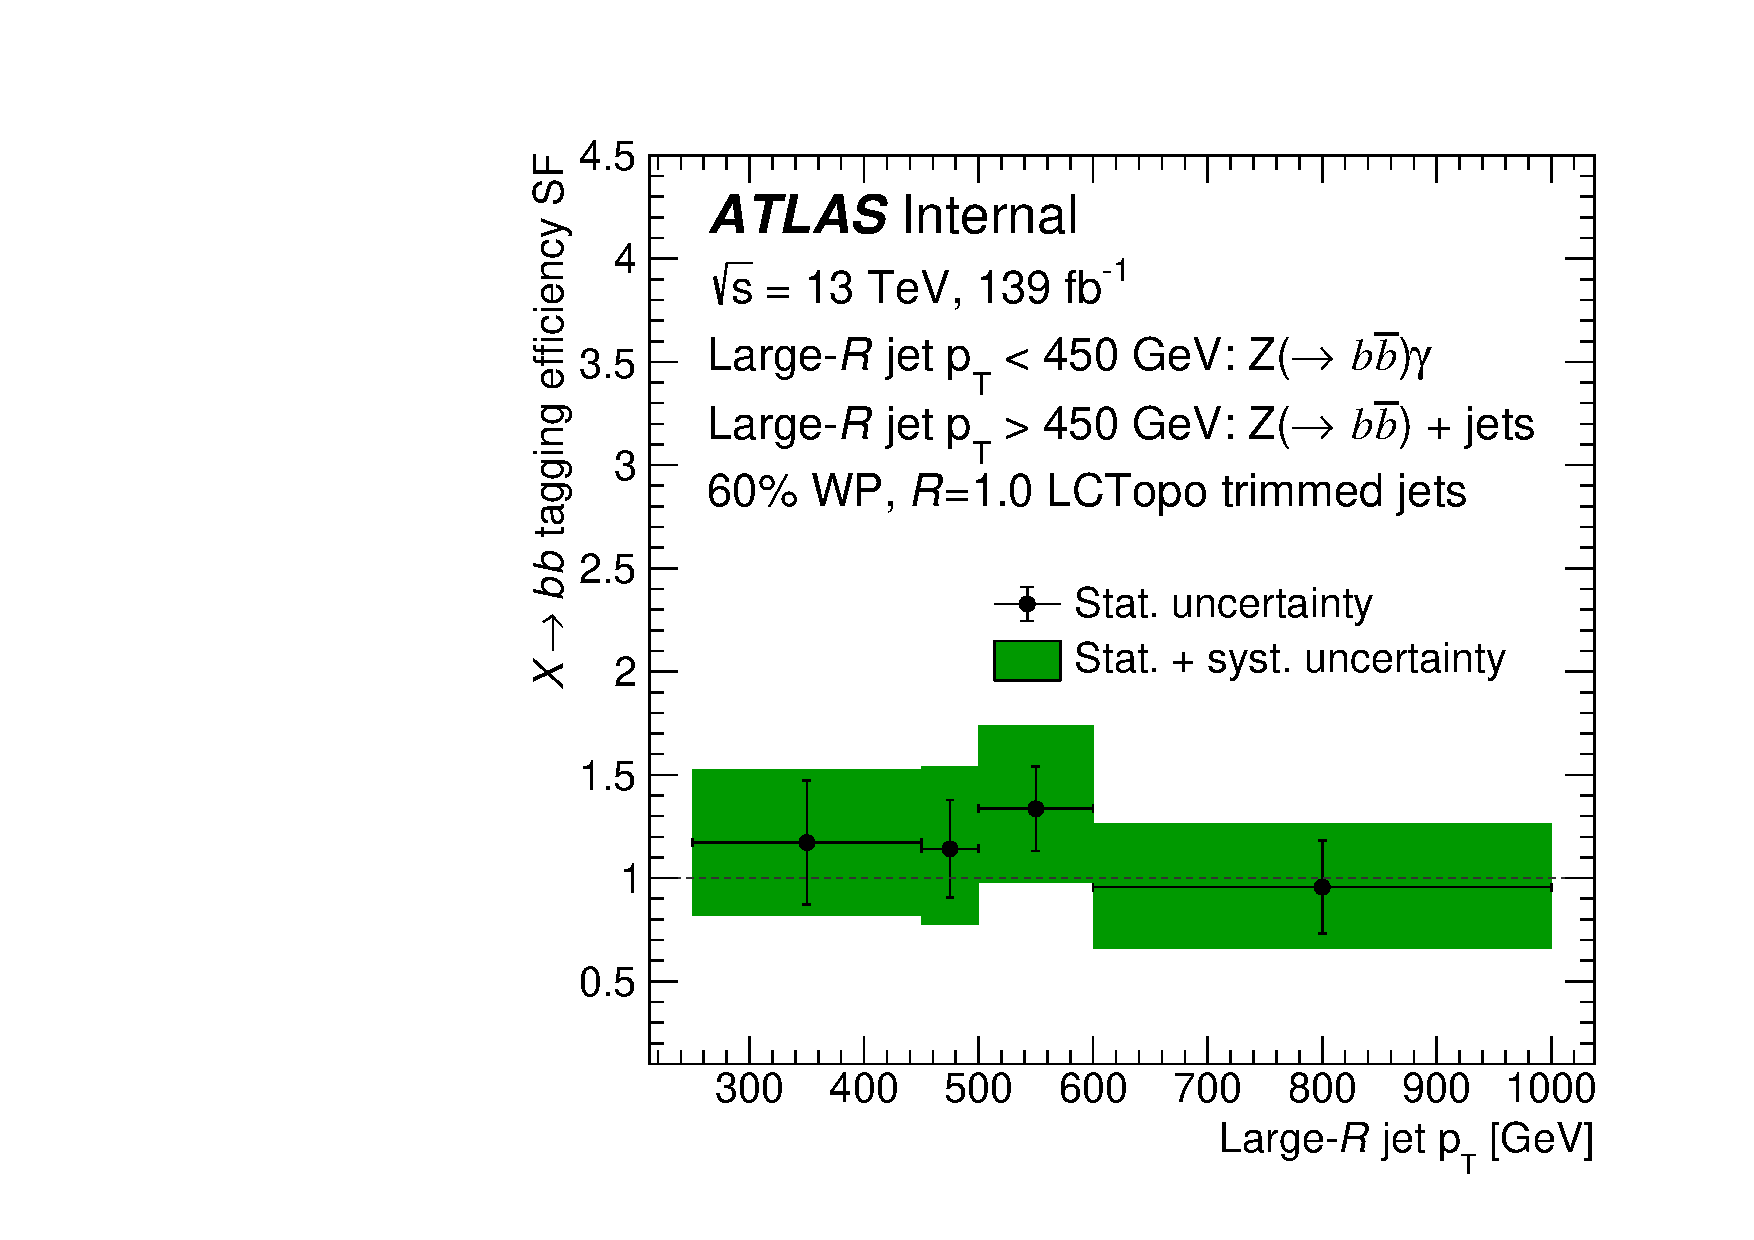
\includegraphics[width=.49\textwidth]{SF_Xbb60_internal_09March2023}} 
\caption[]{Derived scale factors in large-$R$ jet \pt for the \textbf{(a)} \qty[]{50}{\percent} and \textbf{(b)} \qty[]{60}{\percent} \ac{wp} from the calibration of the $X\rightarrow bb$ tagger.}
\label{fig:xbb_sf}    
\end{figure}

\section{Theory Uncertainties}

\section{Background Uncertainties}







theory errors
methodische errors, bkg unc

this analysis driven by stats

modelling errors

statistical unc sqrt(w) blah

luminosity

\section{Reconstruction Uncertainties}

\chapter{Statistics}\label{sec:statistics}

Every scientific investigation starts with a hypothesis that is to be tested empirically. The main objective is to evaluate if the proposed hypothesis agrees or disagrees with observed data, to either accept or reject it against the null-hypothesis which represents a baseline scenario where only known phenomena are presumed to occur.

A key metric that quantifies this is the p-value that arises within hypothesis testing. Test results of an experiment follow some probability density function. Assuming some hypothesis, the p-value is the integrated probability for test results compatible with this hypothesis and ergo measuring the compatibility of the observation to the assumption. In other words if the experiment where to be repeated it gives the probability that the result favors the proposed hypothesis.

In the field of high energy physics a framework has been developed specifically for this task. This section begins to lay out the mathematical fundamentals of the approach and explains its implementation in \textsc{pyhf} \citep{pyhf,pyhf_joss}. The following is based on \citep{cowan2011asymptotic,behnke2013data,pyhf}.

\section{Profile Likelihood Ratio}\label{sec:likelihood}
The statistical model needs to reflect the compatibility of predictions with the observed collision events. This can be quantified by a likelihood $L(\bm{x} | \bm{\phi})$ which is a probability for an observation $\bm{x}$ under a given set of parameters $\bm{\phi}$ that govern the predictions. Given that this is a counting experiment bins of a histogram $\bm{h}=(h_1,...,h_N)$ are the main tool of analysis.

The observation can be subdivided $\bm{x}=(\bm{n},\bm{a})$ into observable histograms $\bm{n}$ and auxiliary measurements. Observable histograms could be the invariant mass of a particle on the other hand auxiliary measurement histograms $\bm{a}$ can be any additional observable that assist in constraining the model. For instance they can be a measurement of a kinematic variable in a phase space region where only background is expected. It should be noted that these auxiliary measurements are not equivalent to the inclusion of uncertainties into the model. The treatment of uncertainties is addressed separately in section \ref{sec:histfactory_model}.

Another useful splitting for the set of parameters $\bm{\phi}=(\bm{\psi},\bm{\Theta})$ into so-called parameters of interest $\bm{\psi}$ and nuisance parameters $\bm{\Theta}$. For this section only one parameter of interest is considered, the signal strength $\mu$.

The bin contents can then be expressed in terms of the amount of signal $s_i(\bm{\Theta})$ and background $b_i(\bm{\Theta})$ in bin $i$ that depend on the nuisance parameters. The prediction (expectation value) of the histogram bins of the observable $n_i$ can then be expressed as
\begin{equation} \label{eq:n_i}
    \langle n_i(\mu,\bm{\Theta})\rangle = \mu s_i(\bm{\Theta}) +b_i(\bm{\Theta}).
\end{equation}
Similarly for auxiliary measurement bins $a_i$ their expectation value are calculable from some function $u_i(\bm{\Theta})$ modeling some observable and is also dependent on the nuisance parameters
\begin{equation} \label{eq:a_i}
    \langle a_i(\bm{\Theta}) \rangle = u_i(\bm{\Theta}).
\end{equation}
Since this is a counting experiment in which events occur at a constant mean rate and independently of time each bin follows a Poisson distribution
\begin{equation}\label{eq:poisson}
    P(r,k)=\frac{r^k e^{-r}}{k!}.
\end{equation}
$r$ is the expected rate of occurrences which translates as the prediction whereas $k$ are the actual measured occurrences. A likelihood can then be constructed from a product of Poisson probabilities
\begin{equation}\label{eq:likelihood}
    L(\mu,\bm{\Theta})=
    \prod_{j=1}^N \frac{(\mu s_j(\bm{\Theta}) + b_j(\bm{\Theta}))^{n_j}}{n_j !} e^{-(\mu s_j(\bm{\Theta}) + b_j(\bm{\Theta}))}
    \prod_{k=1}^M \frac{u_k(\bm{\Theta})^{a_k}}{a_k!} e^{-u_k(\bm{\Theta})}.
\end{equation}
The last product can also be thought of penalizing the likelihood if e.g. an auxiliary measurement displays a very improbable value for some quantity. To test for a hypothesized value of $\mu$, the best choice according to the Neyman-Pearson lemma \citep{behnke2013data}, is the profile likelihood ratio that reduces the dependence to the parameter(s) of interest
\begin{equation}\label{eq:likelihood_ratio}
    \lambda(\mu)=
    \frac{L(\mu,\hat{\hat{\bm{\Theta}}})}
    {L(\hat{\mu},\hat{\bm{\Theta}})}.
\end{equation}
The denominator is the unconditional maximum likelihood estimate so that $\hat{\mu}$ and $\hat{\bm{\Theta}}$ both are free to vary to maximize $L$, whereas the numerator is the found maximum likelihood conditioned on some chosen $\mu$ and the set of nuisance parameters $\hat{\hat{\bm{\Theta}}}$ that maximize the likelihood for that particular $\mu$. This definition gives $0 \leq \lambda \leq 1$ where $\lambda = 1$ corresponds to perfect agreement of the hypothesized value of $\mu$ to the model.

\section{Test Statistic and p-value}
To test for alternative hypotheses it is useful to transform the profile likelihood into a test statistic
\begin{equation}
    t(\mu)=-2\ln \lambda(\mu).
\end{equation}
This translates to $t \rightarrow 0$ as increasing agreement and $t \rightarrow \infty$ as decreasing agreement to the model. A right-tail p-value can then be calculated from the probability density function of the test statistic: \ac{pdf}$(t) = f(t | \mu)$
\begin{equation}\label{eq:p-value}
    p= \int_{t_\text{obs}}^{\infty}
    f(t | \mu) \mathrm{d}t
\end{equation}
$t_\text{obs}$ is the test statistic $t$ evaluated at the observed data which means replacing the predictions in the likelihood of the numerator of equation \ref{eq:likelihood_ratio} with the values observed in data. Similar to the \ac{pdf} of a standard normal distribution the \ac{pdf} in this context quantifies how probable a particular value of the test statistic $t$ is under a fixed value of the signal strength. This essentially measures how frequently a particular value of $t$ occurs in comparison to all other possible values that $t$ can take.

To calculate p-values the integral of equation \ref{eq:p-value} must be solved. The test statistic's specific form is useful because of existing approximations for $f(t | \mu)$ \citep{cowan2011asymptotic}. Let $f(t | \mu')$ be the probability distribution for the true strength parameter $\mu'$. \citet{wald1943tests} demonstrated that for a single parameter of interest the test statistic is equivalent to a normalized sum of squared distances between the tested parameter $\mu$ and its maximum likelihood estimate $\hat{\mu}$
\begin{equation}
    t(\mu)=-2\ln \lambda(\mu)=
    \left(\frac{\mu-\hat{\mu}}{\sigma_{\hat{\mu}}} \right)^2
    + \mathcal{O}(\frac{1}{\sqrt{N}}).
\end{equation}
The maximum likelihood estimate $\hat{\mu}$ is in the large sample limit normally distributed around their true value $\mu'$ with standard deviation $\sigma_{\hat{\mu}}$. This is the definition of a $\chi$-squared distribution with one degree of freedom. It can be shown that \citep{cowan2011asymptotic} the \ac{pdf} of $t$ is  asymptotically follows
\begin{equation}\label{eq:chi-square}
    f(t | \mu)=\frac{1}{2\sqrt{t}}\frac{1}{\sqrt{2\pi}}
    \left[
        \exp\left(-\frac{1}{2}\left(\sqrt{t}+\sqrt{\Lambda}_\mu\right)\right)
        +
        \exp\left(-\frac{1}{2}\left(\sqrt{t}-\sqrt{\Lambda}_\mu\right)\right)
        \right],
\end{equation}
with the non-centrality parameter as the normalized distance between the tested $\mu$ and true parameter of interest $\mu'$
\begin{equation}
    \Lambda_\mu=\frac{(\mu-\mu')^2}{\sigma^2}.
\end{equation}
Figure \ref{fig:test_stat_example} illustrates these steps. Being able to calculate p-values allows to state how likely it is that the proposed hypothesis is reflected by the observed data. In other words, the p-value represents the probability, how incompatible the proposed hypothesis or prediction is with the observation.
\begin{figure}
    \centering
    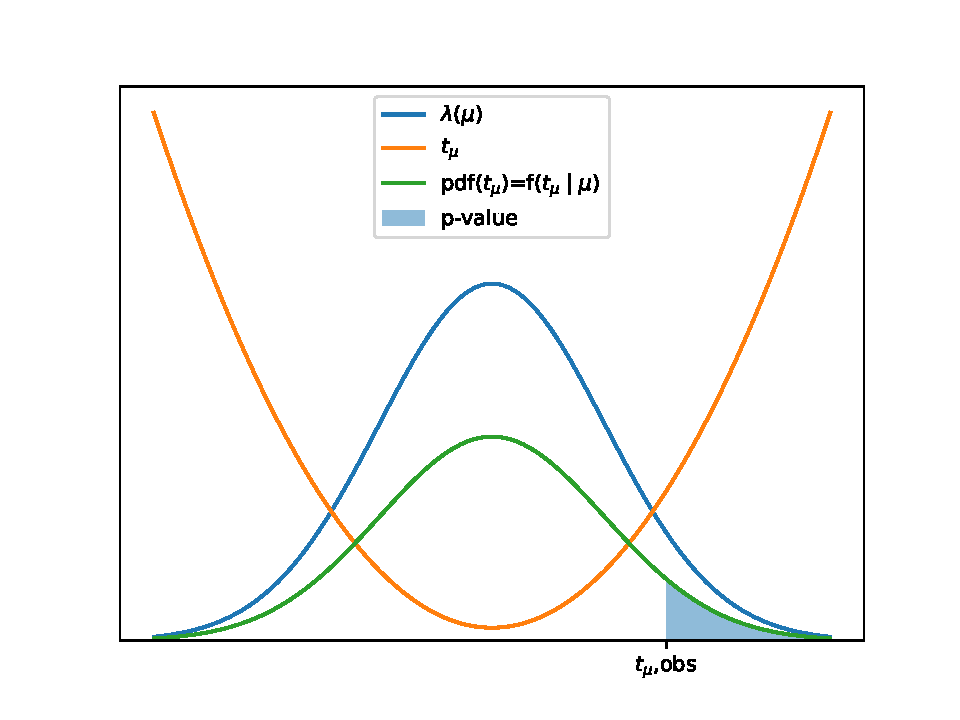
\includegraphics[width=0.8\textwidth]{test_stat_example.pdf}
    \caption[]{A sketch to follow the steps to calculate p-values. (\textbf{left}) The profile likelihood ({\color[HTML]{1f77b4}{$\bm{\diagup}$}}) has essentially some hill-like form with a maximum at ${\lambda(\hat{\mu},\hat{\bm{\Theta}})}$. The test statistic $t$ ({\color[HTML]{ff7f0e}{$\bm{\diagup}$}}) is calculated as $-2\mathrm{ln}(\lambda)$. (\textbf{right}) For one parameter of interest in the large sample limit $f(t | \mu)$ from equation \ref{eq:chi-square} follows a non-central chi-squared distribution with one degree of freedom. The blue shaded area under the \acp{pdf} is a right hand sided p-value.}
    \label{fig:test_stat_example}
\end{figure}

In the scientific community a p-value of 0.05 is commonly accepted as significant. Though particle physicists only claim discovery of a new phenomenon for $p$ < \qty{2.87e-7}{} corresponding to 5 standard deviations of the standard normal distribution and exclude hypotheses if the p-value is not below 2 standard deviations of the standard normal distribution $p$ $\lesssim$ \qty{0.05}{}. A key consideration is that $t$ can assume negative values for $\mu$ which might be non-physical depending on the context. This is handled by cutting off the test statistic for undesired behavior. An example of an adjusted test statistic for setting upper limits is
\begin{equation}
    q_\mu=
    \begin{cases}
        -2\ln \lambda(\mu) & \hat{\mu}\leq\mu \\
        0                  & \hat{\mu}> \mu
    \end{cases}.
\end{equation}
Here if a tested signal strength $\mu$ is not larger than the maximum estimate it would not be regarded as less compatible and is therefore set to zero. Various cases and approximations of \acp{pdf} in different scenarios are detailed in \citep{cowan2011asymptotic}.

\section{The CL$_s$ value}\label{sec:cls}
Particle physicists typically concentrate on two key aspects when performing statistical tests to discover new phenomena: the accurate modeling of known backgrounds and whether there is evidence in the observations for a new phenomenon. This involves assessing two distinct hypotheses: a background only ($b$) and one that involves signal and background ($s+b$). Each will result in a p-value of their own.

For example, a p-value of $p_{b} = 0$ would indicate a perfect modeling of the background model reflected in observational data, meaning that known phenomena have been accurately accounted for. Conversely, a p-value of $p_{s+b} < 0.05$ might signal the presence of new phenomena, such as previously undiscovered physics.

To synthesize these two aspects into a unified metric particle physicists developed a pseudo Confidence Level/p-value referred to as CL$_s$. This measure not only considers the potential presence of new phenomena but also the accuracy of the background modeling.
\begin{equation}
    \mathrm{CL}_s=\frac{p_{s+b}}{1-p_{b}}=
    \frac
    {\int_{t_\text{obs}}^{\infty}
        f(t_{s+b} | \mu) \mathrm{d}t}
    {1-\int_{t_\text{obs}}^{\infty}
        f(t_{b} | \mu) \mathrm{d}t}.
\end{equation}
The numerator represents the p-value for the alternative hypothesis while the denominator p-value penalizes the CL$_s$ based on how compatible the background model is with the observational data.  This concept can also be understood visually from the first figure of the paper that introduced the CL$_s$ quantity \citep{read2002presentation} and is explained here in figure \ref{fig:cls}.
\begin{figure}
    \centering
    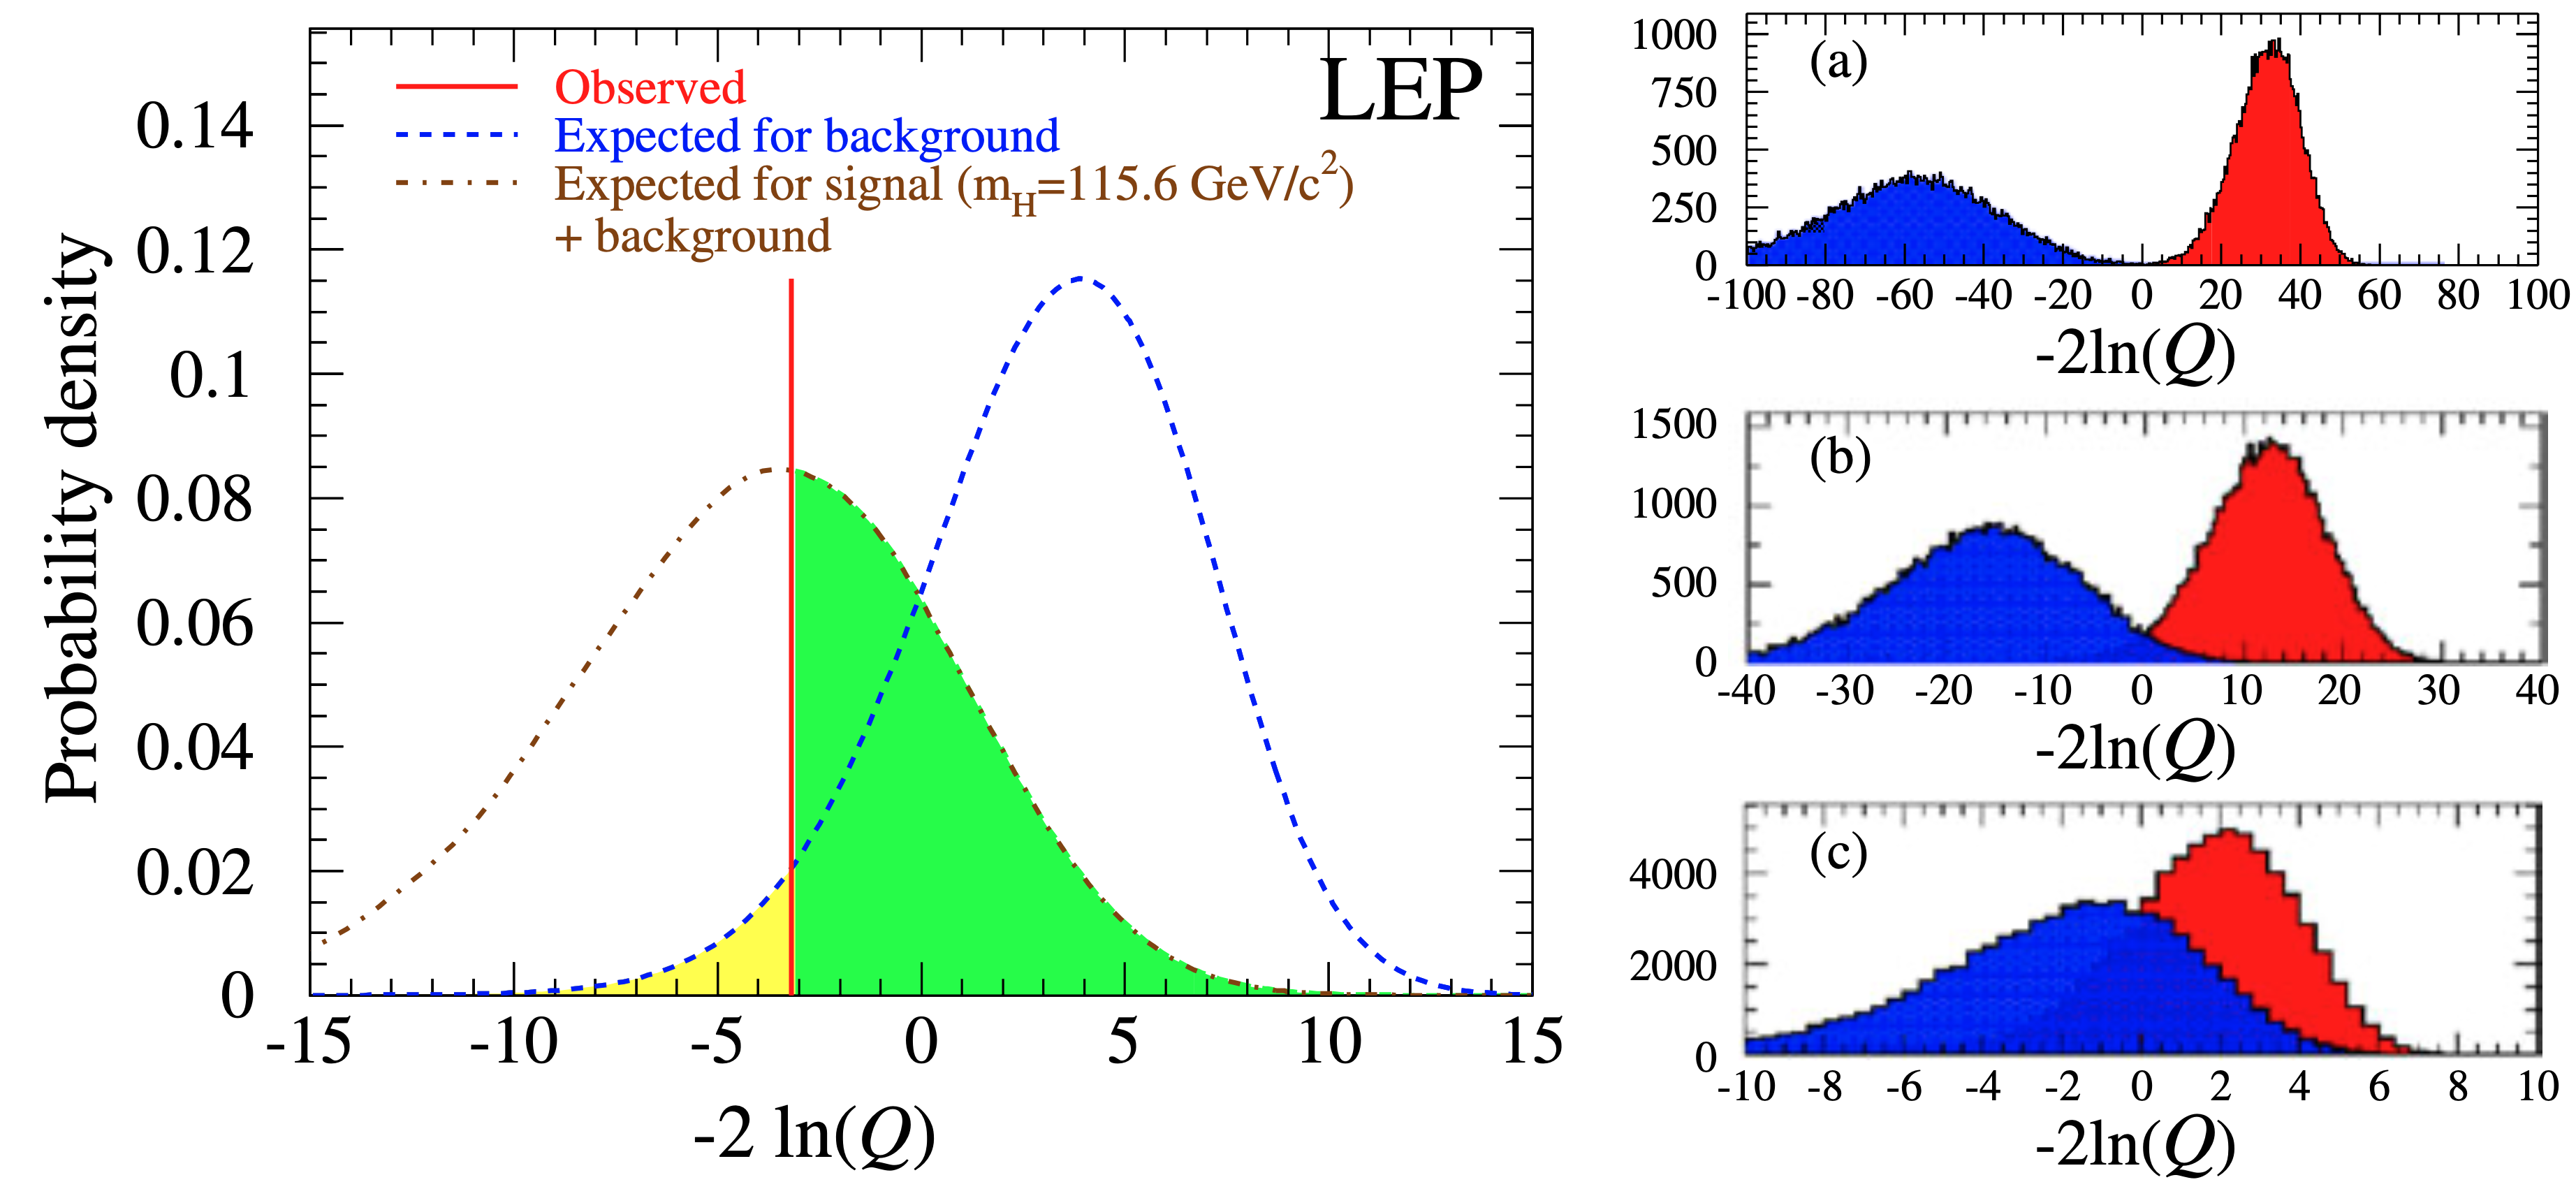
\includegraphics[width=1\textwidth]{cls.png}
    \caption[]{Probability density functions of test statistics from a Higgs search at LEP illustrating the calculation of p-values ($\lambda$ becomes $Q$). (\textbf{left}) The \acp{pdf}'s of the test statistic $f(t | \mu)$ of the signal + background ({\color[HTML]{804000}{$\bm{\diagup}$}}) and background ({\color[HTML]{2100FF}{$\bm{\diagup}$}}) only hypotheses. The p-value is calculated by integration from $t_\text{obs}$ (the red observed line ({\color[HTML]{FF0000}{$\bm{\diagup}$}})) to infinity (see eq. \ref{eq:p-value}). The green shaded area (\hexbox{00FF00}) corresponds to $p_{s+b}$ whereas the yellow area (\hexbox{FDFF02}) corresponds to $1-p_b$ since the integral over one whole \acp{pdf} is 1. (\textbf{right}) Degradation of search sensitivity from (a) to (c). Note that the colors of the \acp{pdf}'s change here to signal + background (\hexbox{2100FF}) and background only (\hexbox{FF0000}). For example putting the observation ($t_\text{obs}$) on the x-axis at 0 in these plots, one would get for plot (a) $p_{b}\approx 1$ and $p_{s+b}\approx 0$ resulting in a CL$_s\approx 0$, whereas with increasing overlap the CL$_s$ value increases and the sensitivity decreases. Adopted from \citep{read2002presentation}.}
    \label{fig:cls}
\end{figure}


\section{HistFactory}\label{sec:histfactory_model}
A widely-used model for constructing likelihoods as discussed in section \ref{sec:likelihood} is known as HistFactory \citep{cranmer2012histfactory}. This model is implemented in the \textsc{pyhf} toolkit \citep{pyhf} and the following section is primarily based on the introduction to HistFactory found in the \textsc{pyhf} documentation. HistFactory simplifies the process of building a likelihood by breaking it down into several fundamental components. To understand this it is helpful to consider a different categorization of the model parameters $\bm{\phi}$
\newcommand{\freeset}{\bm{\eta}}
\newcommand{\constrset}{\bm{\chi}}
\newcommand{\singleconstr}{\chi}
\newcommand{\channelcounts}{\bm{n}}
\newcommand{\auxdata}{\bm{a}}
\newcommand{\poiset}{\bm{\psi}}
\newcommand{\nuisset}{\bm{\theta}}
\newcommand{\fullset}{\bm{\phi}}
\newcommand{\singlefull}{\phi}
\begin{equation}
    L(\bm{x}|\fullset) \quad=\quad
    L(\bm{x}|\overbrace{\poiset}^{\llap{\text{parameters of interest}}},\underbrace{\nuisset}_{\llap{\text{nuisance parameters}}}) \quad=\quad
    L(\bm{x}|\overbrace{\freeset}^{\rlap{\text{free}}},\underbrace{\constrset}_{\rlap{\text{constrained}}}),
\end{equation}
Free parameters $\freeset$ are free to choose in the model and can be for example a cross-section of a process. Constrained parameters $\constrset$ are used to incorporate uncertainties into the likelihood to constrain it. Further there might be several histograms of an observable, for example measured in orthogonal kinematic regions, that are called channels $c$. Bins have the index $b$ here and constraint terms are denoted $c_{\singleconstr}$. The likelihood can thus be described by
\begin{equation}
    L(\channelcounts, \auxdata \,|\,\freeset,\constrset)
    = \underbrace{\color{blue}{\prod_{c\in\mathrm{\,channels}} \prod_{b \in \mathrm{\,bins}_c}
            \textrm{Pois} ( 
                \;\overbrace{n_{cb}}^{\llap{\text{\strut observed}\quad\;}}
            \,|\, \overbrace{\nu_{cb}\left(\freeset,\constrset\right)}^{\llap{\quad\text{\strut predicted}}}
            \;)}}_{\substack{\text{Simultaneous measurement}\\%
            \text{of multiple channels}}}
    \underbrace{\color{red}{\prod_{\singleconstr \in \constrset} c_{\singleconstr}(a_{\singleconstr} |\, \singleconstr)}}_{\substack{\text{constraint terms}\\%
            \text{for }\text{auxiliary measurements}}}.
            \label{eq:histfactory_likelihood}
\end{equation}
$\bm{n}$ and $\bm{a}$ are the observations auxiliary measurement hisograms as defined in section \ref{sec:likelihood}. The $n_{cb}$ is the observed bin content and $\nu_{cb}(\freeset,\constrset)$ the predicted bin content. $c_{\singleconstr}(a_{\singleconstr} |\, \singleconstr)$ are functions that calculate a probabilistic impact to the likelihood $L$ of uncertainties $a_\chi$ to constrain the parameter $\singleconstr$ and are discussed in detail section \ref{sec:constraint_terms}.

The prediction is a sum of nominal bin counts\footnote{also called rates, like in the definition of a Poisson distribution} $\nu_{scb}^0$ over all samples $s$ (e.g. $t\overline{t}$, multijet-background, etc.). These nominal bin counts are subject to uncertainties. Therefore the bin content can be varied within the bounds of these uncertainties. However the effect of this modification to the likelihood must be taken into account which is through the constraint terms. These penalize the likelihood proportional to the modification. Modifiers are discussed in detail in section \ref{sec:modifiers}. They enter the likelihood through linear modeling of the nominal bin content $\nu_{scb}^0$ with multiplicative $\kappa_{scb}$ and additive modifiers $\Delta_{scb}$ 
\begin{align}
    \nu_{cb}\left(\freeset,\constrset\right) & = \sum_{s\in\mathrm{\,samples}} \nu_{scb}\left(\freeset,\constrset\right)                                                                                                \\
                                             & = \sum_{s\in\mathrm{\,samples}}\underbrace{\left(\prod_{\kappa\in\,\bm{\kappa}} \kappa_{scb}\left(\freeset,\constrset\right)\right)}_{\text{multiplicative modifiers}}\,
    \Bigg(\nu_{scb}^0 + \underbrace{\sum_{\Delta\in\bm{\Delta}} \Delta_{scb}\left(\freeset,\constrset\right)}_{\text{additive modifiers}}\Bigg).
    \label{eq:modifier_equation}
\end{align}
The usefulness of this approach becomes clear when considering one uncertainty $a_\chi$ on a nominal bin count estimate $\nu_{scb}^0$. The main goal remains to maximize the overall likelihood $L$. This can be achieved via maximizing the Poisson probability (blue part in equation \ref{eq:histfactory_likelihood}) and at the same time keeping the constraint term (red part in equation \ref{eq:histfactory_likelihood}) large. It is illustrative to consider one nuisance parameter $\chi$ as a multiplicative modifier $\kappa_{scb}=\chi$ on $\nu_{scb}^0$. An optimum can be found by modifying the prediction to move closer to the observed value (blue part in equation \ref{eq:histfactory_likelihood}) while at the same time keeping the constraint term $c_\kappa(\kappa)$ (red part in equation \ref{eq:histfactory_likelihood}) controlled by the same $\chi$ at values where the penalization of the likelihood stays insignificant. This works well for example when $\kappa$ has a very large uncertainty rendering the constraint term's influence on the likelihood relatively small. 

\subsection{The Modifiers}\label{sec:modifiers}
In HistFactory there are by convention four types $\{\lambda,\mu,\gamma,\alpha\}$ of such multiplicative rate modifiers that are explained in this section. There are \textbf{free rate modifiers} for the luminosity $\lambda$ and signal strength $\mu$ that affect all bins equally
\begin{equation}
    \nu_{scb}(\mu)=\mu \nu_{scb}^0.
\end{equation}
These are bin-independent normalization factors and preserve the shape of the histogram.
Further there are \textbf{bin-wise modifiers} $\gamma_b$ (uncorrelated shape)
\begin{equation}
    \nu_{scb}(\gamma_b)=\gamma_b \nu_{scb}^0.
\end{equation}
These are useful for example to include uncertainties of a per bin data-driven background estimate. This type without a constraint term is not of much use as if there is only one sample or channel, the fit would always match the data perfectly.
In addition there exist \textbf{interpolation parameters $\alpha$} (shape factors) that enter the modeling through an interpolation function $\eta$ instead of being the factor itself. They exist in multiplicative versions
\begin{equation}
    \nu_{scb}(\alpha)=\eta(\alpha) \nu_{scb}^0,
\end{equation}
and additive versions
\begin{equation}
    \nu_{scb}(\alpha)=\nu_{scb}^0 + \eta(\alpha).
\end{equation}
This is useful to include systematic uncertainties. Typically they are known for one standard deviation of a bin count $\eta_{-1}=\nu_{scb}^\mathrm{1down}$ and $\eta_{1}=\nu_{scb}^\mathrm{1up}$ to the nominal value $\nu_{scb}^0$. These are then used to construct interpolation functions that modify the nominal value controlled by the nuisance parameter that also controls the constraint term $c_\alpha$ which is further explained in section \ref{sec:constraint_terms}. Thus one parameter controls the modification and constraint at a time.

In HistFactory there exists four of such interpolation functions. For those exist an identity operator
\begin{equation}
    \eta_0=\eta (\alpha=0) =
    \begin{cases}
        1 , & \text{multiplicative modifier, } (\kappa) \\
        0 , & \text{additive modifier, } (\lambda).
    \end{cases}
\end{equation}
One example of these interpolation functions that scales the bin count linearly over the known deviations $\eta_{-1}=\nu_{scb}^\mathrm{1down}$ and $\eta_{1}=\nu_{scb}^\mathrm{1up}$ is
\begin{equation}
    \eta_\mathrm{linear}(\alpha)=
    \begin{cases}
        \alpha(\eta_0 - \eta_1) ,    & \alpha>0 \\
        \alpha(\eta_0 - \eta_{-1}) , & \alpha<0
    \end{cases}
\end{equation}
This is illustrated in fig. \ref{fig:interp_func}(a). For the other ones see e.g. \citep{heinrich2019searches}. It is noted that $\alpha$ is the nuisance parameter and not the function $\eta(\alpha)$ and there is an associated constraint term $c_\alpha$ to each $\alpha$.
\begin{figure}
    \centering
    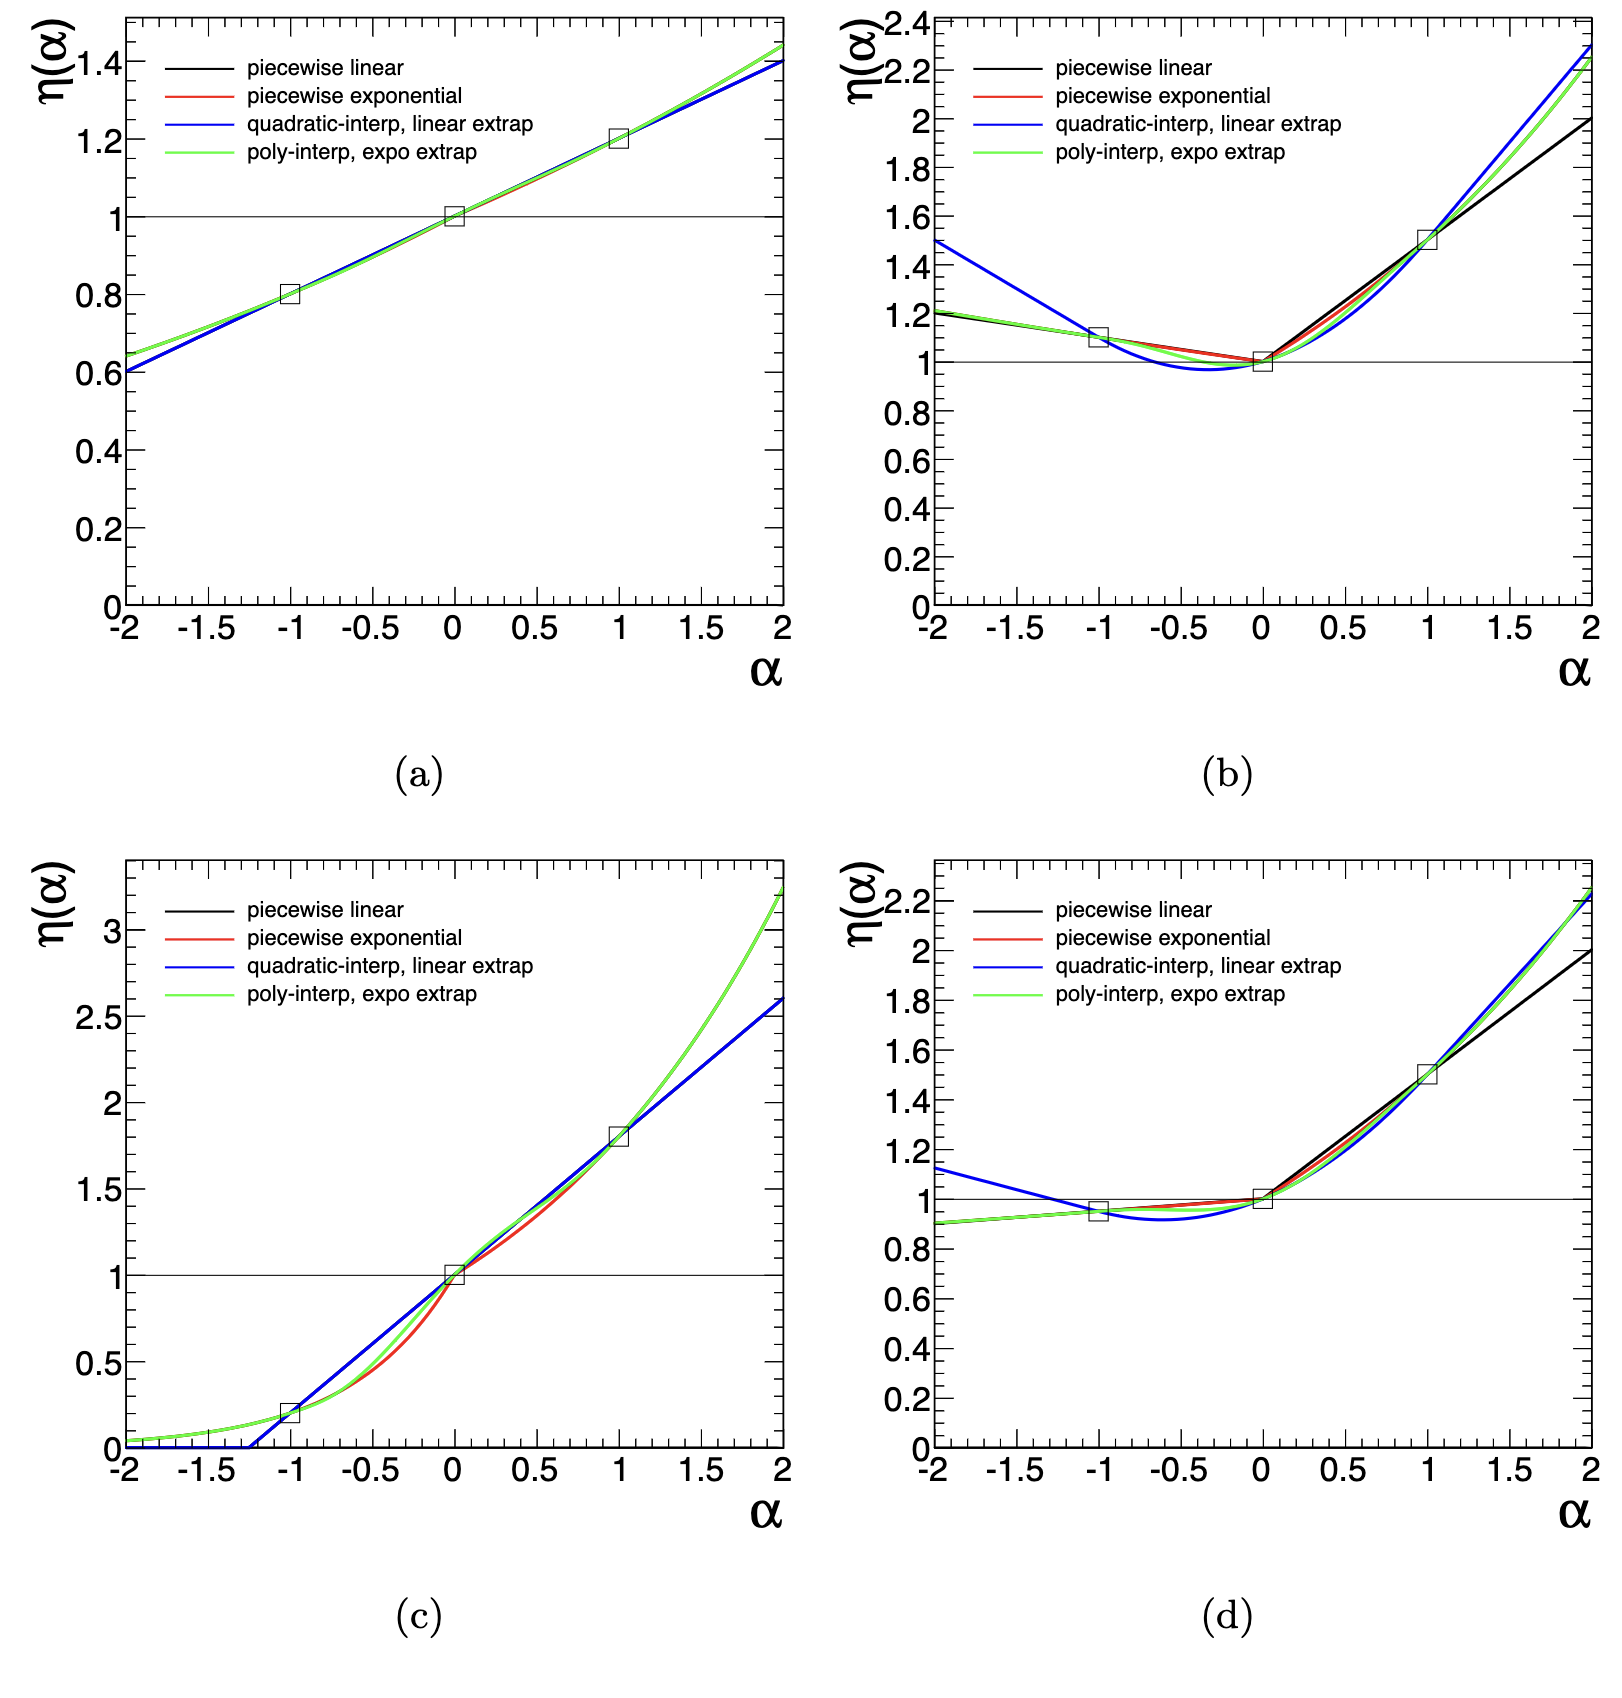
\includegraphics[width=.8\textwidth]{interp_func.png}
    \caption[]{The four interpolation functions $\eta(\alpha)$ for different up and down standard deviation values. For example in (a) the bin count will be scaled with a factor of 0.8 for an $\alpha=-1$ (1.2 for an $\alpha=1$). From \citep{cranmer2012histfactory}.}
    \label{fig:interp_func}
\end{figure}

\subsection{The constraint terms}\label{sec:constraint_terms}
Uncertainties are modeled either Gaussian or Poissonian. The Gaussian uncertainty implementation is straightforward as the standard deviation $\sigma$ appears in the definition of the Gaussian with mean $\mu$
\begin{equation}
    \text{Gaus}(\mu|x,\sigma)=\frac{1}{\sigma\sqrt{2\pi}}e^{-\frac{1}{2}\left(\frac{x-\mu}{\sigma}\right)^2}.
\end{equation}
So that the likelihood for a Gaussian uncertainty is constrained by a Gaussian scaled to one standard deviation controlled by the nuisance parameter $\alpha$: \mbox{$\mathrm{Gauss}(\alpha | a, \sigma=1)$}.

Similar to the Gaussian uncertainty for an uncertainty that is Poissonian distributed
\begin{equation}
    \text{Pois}(k|r)= \frac{r^k e^{-r}}{k!}.
\end{equation}
the nuisance parameter for a multiplicative factor $\kappa_{scb}=\gamma$ in equation \ref{eq:modifier_equation} should control the Poisson constraint term such that the uncertainty $\sigma$ is reflected by the variance of the Poisson $\text{Var}(\text{Pois})=r=\sigma^2$. This is achieved by scaling the distribution with a factor $f$ which is then solved for the one with the desired uncertainty by evaluating it at the nominal value of the multiplicative modifier $\gamma_0=1$ 
\begin{equation}
    \mathrm{Var}\left[\mathrm{Pois}(k=f\gamma_0 | r=f\gamma)\right]
    =
    r=f\gamma\;\stackrel{\gamma=\gamma_0}{=}\;f\gamma_0=(f\sigma)^2 
    \quad 
    \rightarrow \quad f=(1/\sigma^2).
\end{equation}
Thus a Poissonian constraint term for a multiplicative modifier $\gamma$ with uncertainty $\sigma$ reads \mbox{$\text{Pois}(k=\sigma^{-2}|r=\sigma^{-2}\gamma)$.} This completes the necessities for the HistFactory model. The different types of modifiers and their constraint terms are summarized in table \ref{tab:histfactory}.
\begin{table}[]
    \caption[]{Modifiers and constraint terms used in HistFactory implemented by \textsc{pyhf}. Note that the interpolation functions are called $f_p$ and $g_p$ here instead of $\eta$ as chosen in the full text. Input for the constraint terms are the corresponding uncertainties. Adapted from \citep{pyhf}.}
    \centering
    \resizebox{0.97\textwidth}{!}{
        \begin{tabular}{l|l|l|l}\label{tab:histfactory}
            Description          & Modification                                                                                            & Constraint Term $c_\singleconstr$                                                               & $c_\chi$ input                     \\
            \hline
            Uncorrelated Shape   & $\kappa_{scb}(\gamma_b) = \gamma_b$                                                                     & $\prod_b \mathrm{Pois}\left(k_b = \sigma_b^{-2}\middle|\,r_b = \sigma_b^{-2}\gamma_b\right)$ & $\sigma_{b}$                       \\
            Correlated Shape     & $\Delta_{scb}(\alpha) = f_p\left(\alpha\middle|\,\Delta_{scb,\alpha=-1},\Delta_{scb,\alpha = 1}\right)$ & $\displaystyle\mathrm{Gaus}\left(a = 0\middle|\,\alpha,\sigma = 1\right)$                       & $\Delta_{scb,\alpha=\pm1}$         \\
            Normalisation Unc.   & $\kappa_{scb}(\alpha) = g_p\left(\alpha\middle|\,\kappa_{scb,\alpha=-1},\kappa_{scb,\alpha=1}\right)$   & $\displaystyle\mathrm{Gaus}\left(a = 0\middle|\,\alpha,\sigma = 1\right)$                       & $\kappa_{scb,\alpha=\pm1}$         \\
            MC Stat. Uncertainty & $\kappa_{scb}(\gamma_b) = \gamma_b$                                                                     & $\prod_b \mathrm{Gaus}\left(a_{\gamma_b} = 1\middle|\,\gamma_b,\delta_b\right)$                 & $\delta_b^2 = \sum_s\delta^2_{sb}$ \\
            Luminosity           & $\kappa_{scb}(\lambda) = \lambda$                                                                       & $\displaystyle\mathrm{Gaus}\left(l = \lambda_0\middle|\,\lambda,\sigma_\lambda\right)$          & $\lambda_0,\sigma_\lambda$         \\
            Normalisation        & $\kappa_{scb}(\mu_b) = \mu_b$                                                                           &                                                                                                 &                                    \\
            Data-driven Shape    & $\kappa_{scb}(\gamma_b) = \gamma_b$                                                                     &                                                                                                 &                                    \\
        \end{tabular}
    }
\end{table}


\part{Results}
% \chapter{Studies with the Soft Muon Tagger}
In analyses where final states involve  $b$-quarks, as is the case in this study, heavily rely on the accurate identification of these quarks. Thus ongoing research and development efforts are focused on improving the accuracy and efficiency of this identification process. This chapter presents a study on how muons can contribute to the identification of $b$-quarks in current $b$-tagging algorithms applied to small-$R$ jets.

\section{Soft Muon tagging}
\label{sec:SoftMuonTagging}
Algorithms currently in use for $b$-tagging described in section \ref{sec:b_tagging}, primarily exploit the displaced secondary vertex that is characteristic of the long lifetime of $b$-quarks. Besides vertex finding algorithms muons can be used as indication for the presence of a $b$-hadron. This is because approximately \qty{20}{\percent} of the $b$-jets undergo semi-leptonic decays that involve a muon as exemplified in figure \ref{fig:semileptonicDecay}. The branching fractions for these decays are roughly \qty{11}{\percent} for direct $b$ to muon decays $BR( b \rightarrow \mu \nu X )$ and about \qty{10}{\percent} for cascade decays $BR( b \rightarrow c \rightarrow \mu \nu X )$ \citep{expectedPerformanceAtlas}.
\begin{figure}[]
  \centering
  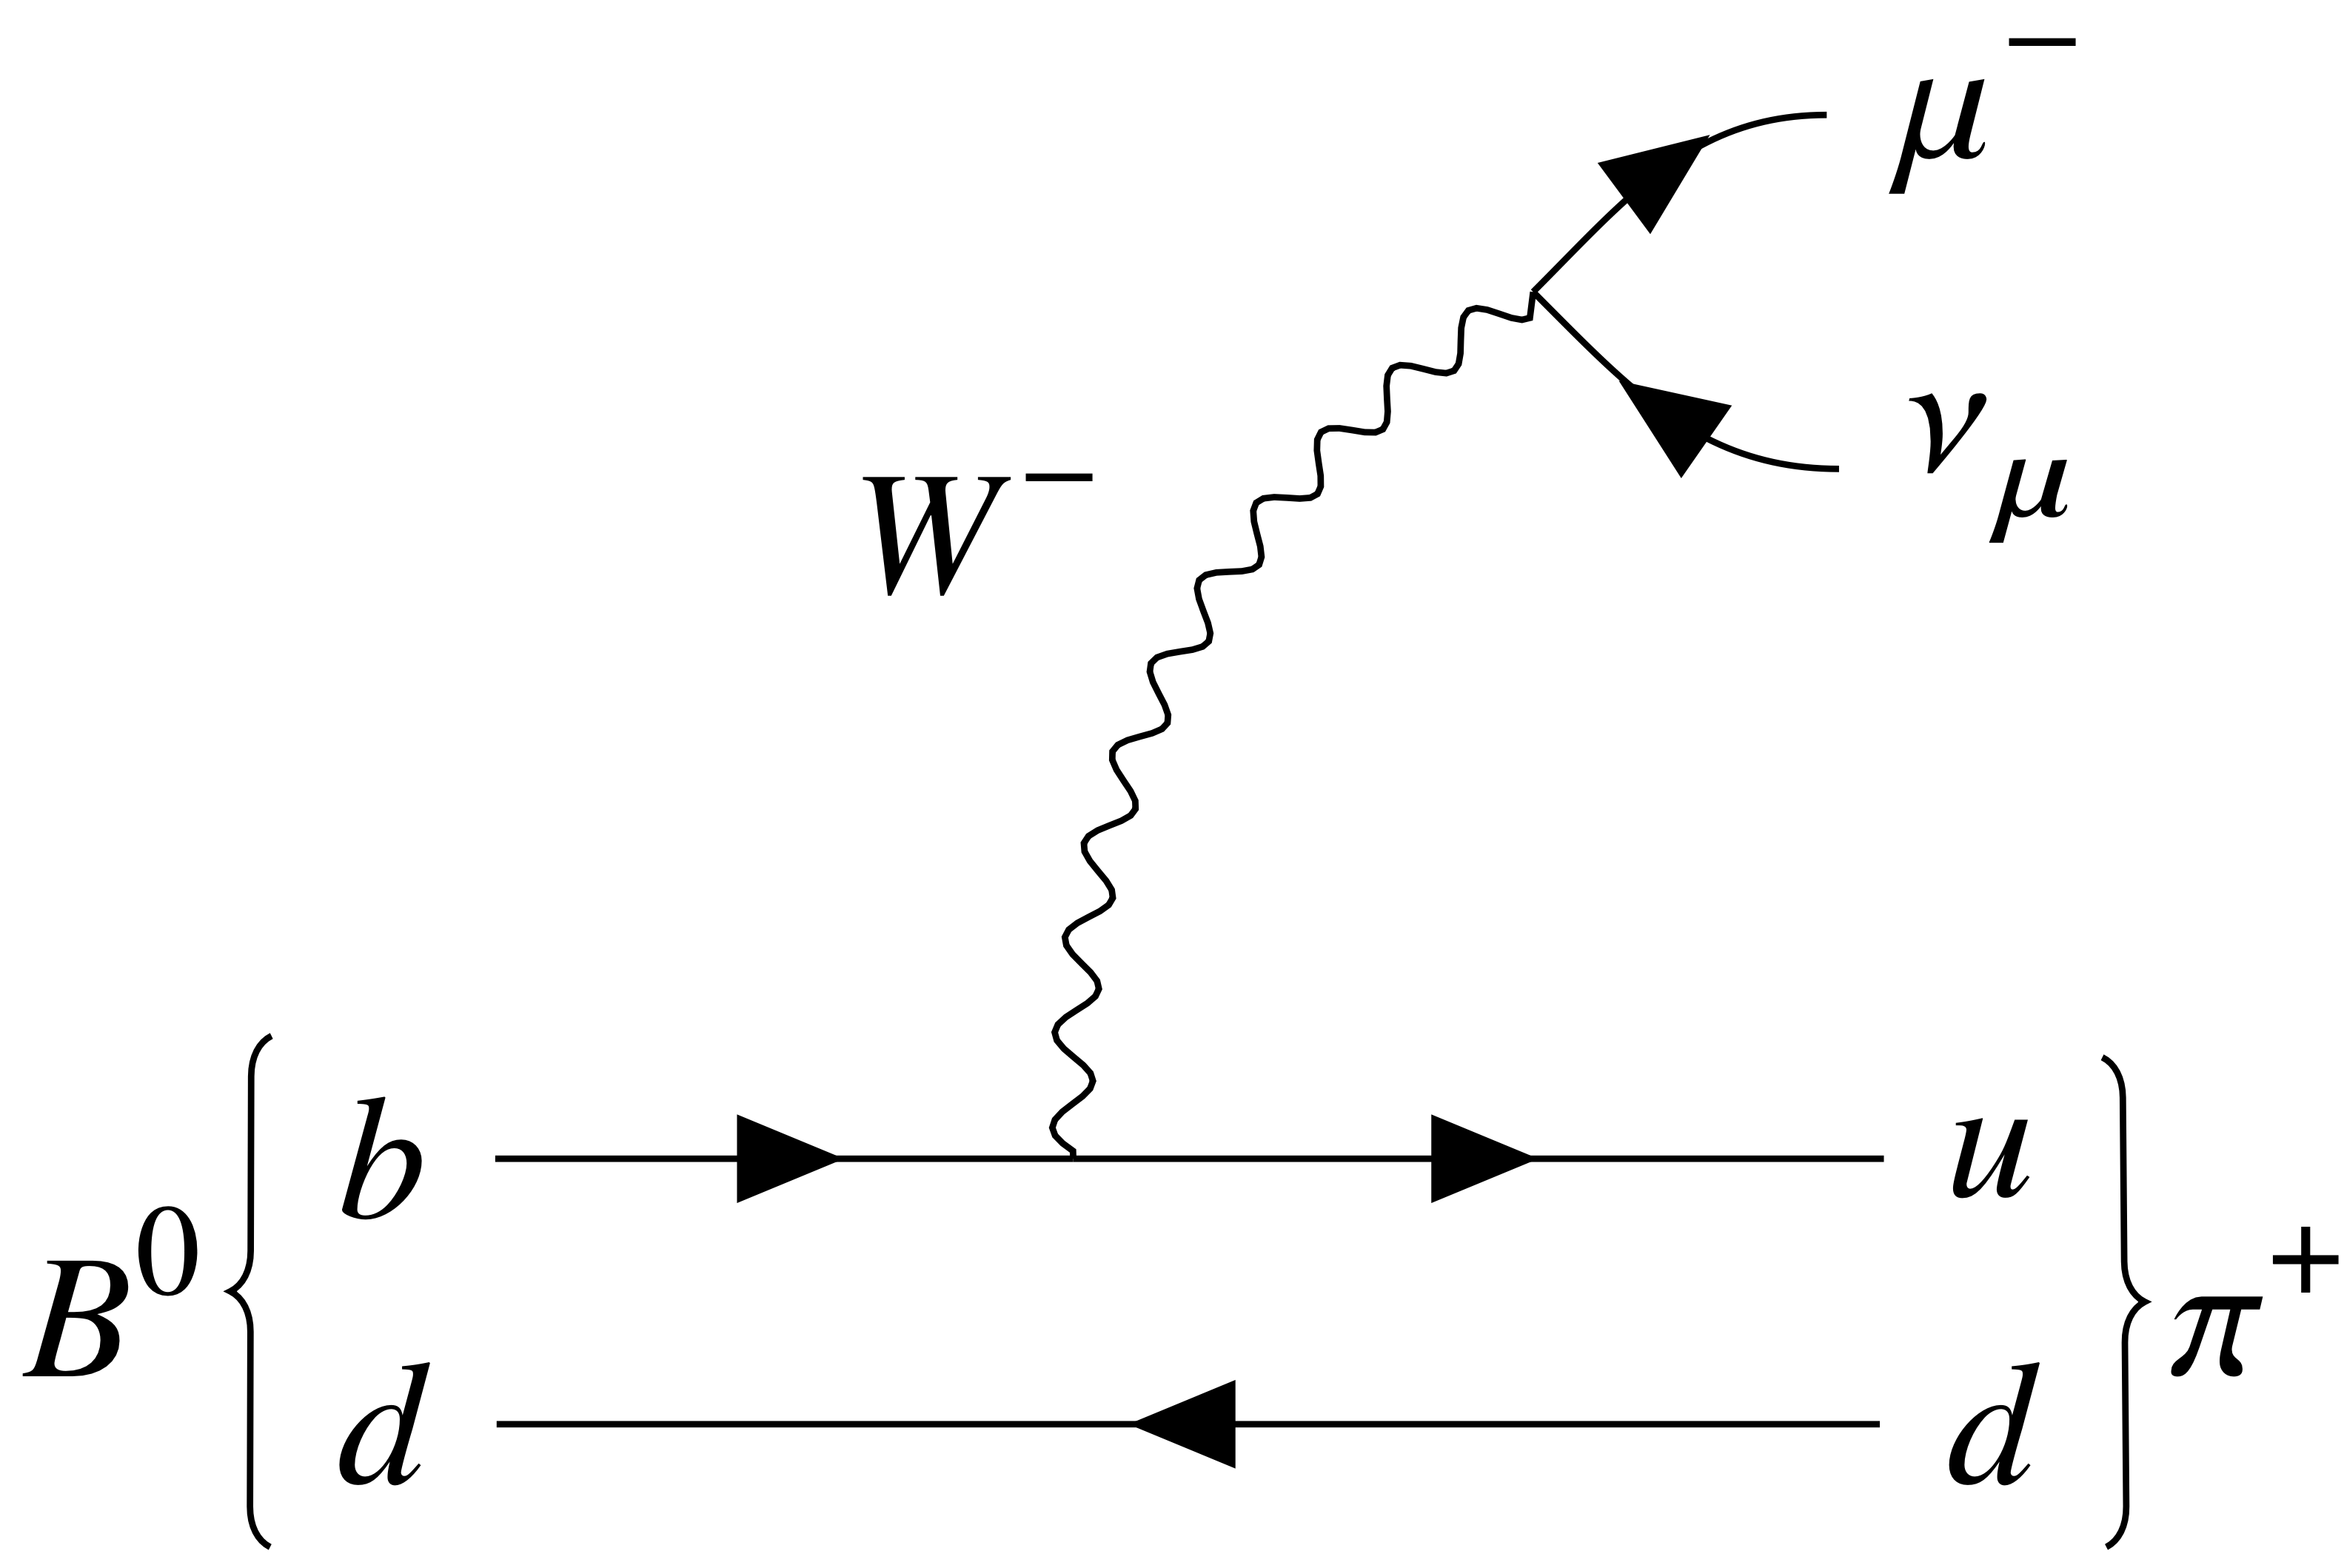
\includegraphics[width=0.4\textwidth]{semileptonic_b_decay}
  \caption{Feynman Diagram depicting a typical semi-leptonic decay of an Anti-$B^0$-meson containing a muon in the final state.}
  \label{fig:semileptonicDecay}
\end{figure}

Despite their limited branching ratio, muons from semi-leptonic heavy-flavor decays are valuable in complementing impact parameter- and vertex-based $b$-tagging methods. These muons typically exhibit higher transverse momentum compared to those from lighter hadron decays, as shown in figure \ref{fig:softMuon_pt}. This relates also to the fact that muons from $b$-decays tend to be more boosted transverse to the jet axis and therefore have a larger orthogonal projection $p_\text{T}^\text{rel}$ of the muon-\pt onto the jet axis. This is calculated by taking the perpendicular part of the three vector muon-momentum to the three-vector jet momentum. The term ``soft'' is derived from the fact that their \pt is smaller than that typically possessed by muons from electroweak boson decays, since they originate from a secondary process \citep{ATL-PHYS-PUB-2017-013}.
\begin{figure}[]
  \centering
  \subfigure[]{
    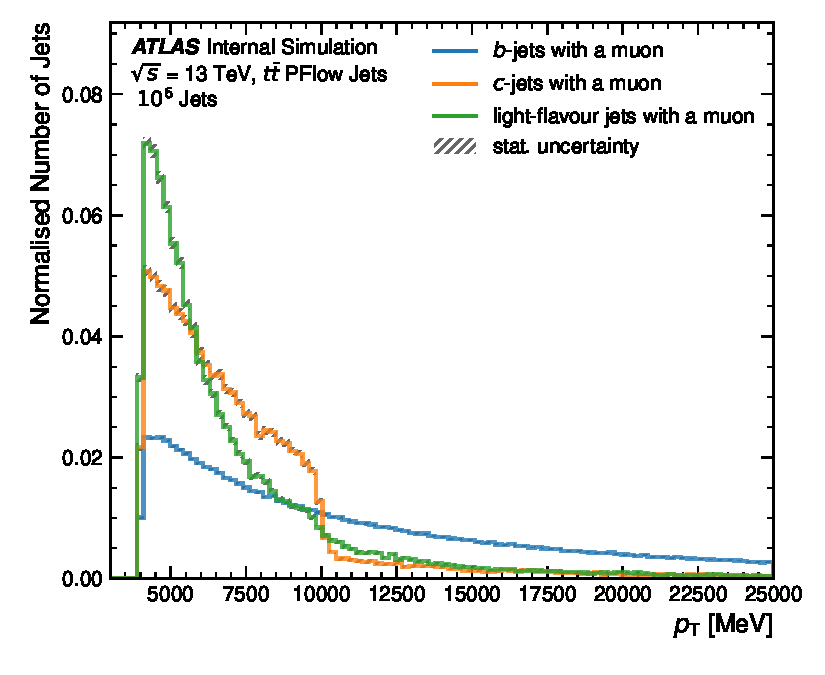
\includegraphics[width=0.45\textwidth]{softMuon_pt}
    \label{fig:softMuon_pt}
  }\hspace*{0.5cm}
  \subfigure[]{
    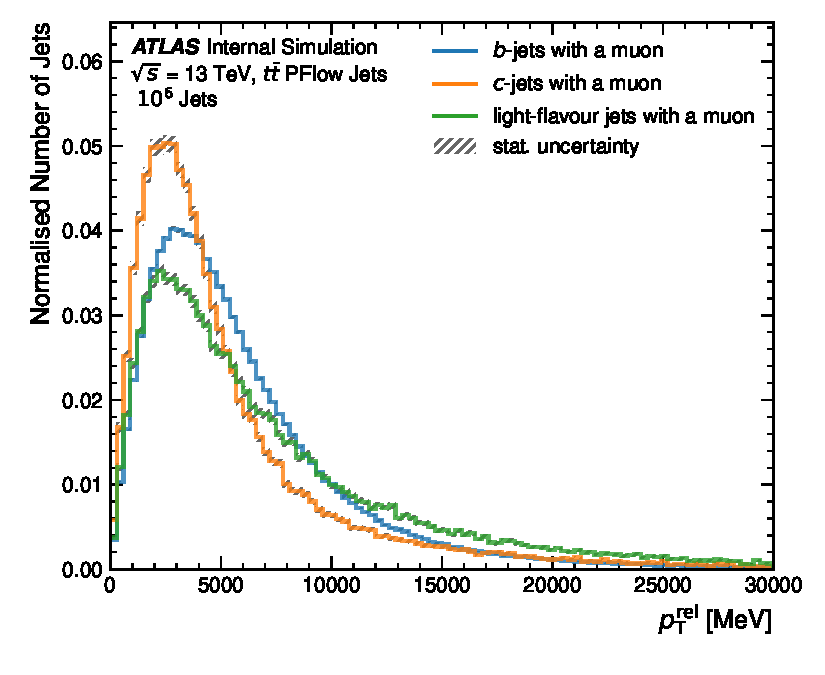
\includegraphics[width=0.45\textwidth]{softMuon_pTrel}
    \label{fig:softMuon_pTrel_sketch}
  }\\
  \subfigure[]{
    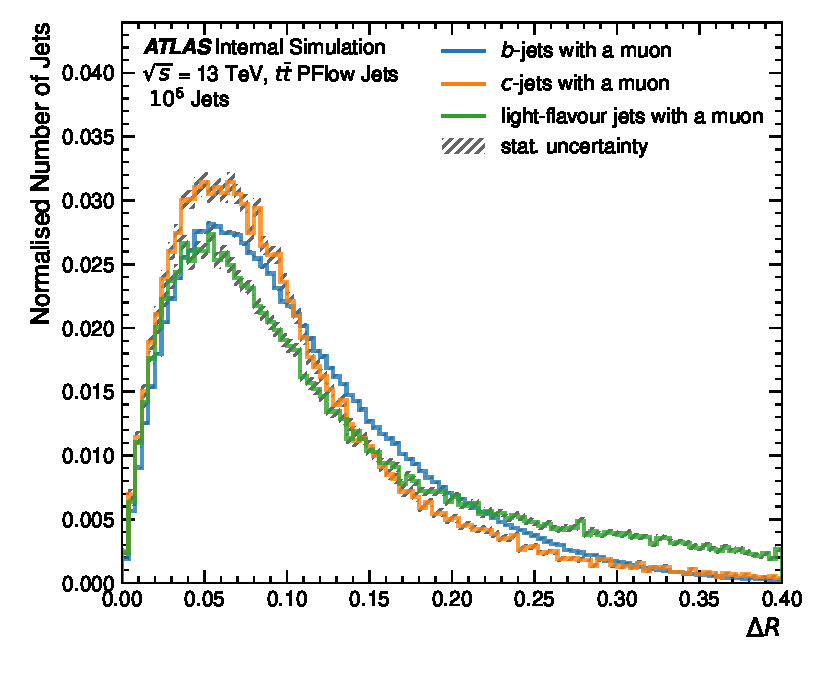
\includegraphics[width=0.49\textwidth]{softMuon_dR}
    \label{fig:softMuon_dR}
  }
  \caption{Kinematics of soft muons: \textbf{(a)} transverse momentum distribution, \textbf{(b)} relative transverse momentum ($p_\text{T}^\text{rel}$) indicative of muons from direct $b$-jet decays being more boosted transversely to the jet axis, and \textbf{(c)} $\Delta R$ distribution between soft muons and jets, normalized per flavor.}
  \label{fig:muonsForSMT}
\end{figure}



% ---------------------------
\section{Muon Selection}
\label{sec:MuonSelection}
%-------------------------------------------------------------------------------
The particle flow algorithm used to reconstruct small-$R$ jets described in section \ref{sec:particle_flow} does not include muons. Thus they are added after jet reconstruction using the shrinking association \DeltaR cone as depicted in figure \ref{fig:shrinkCone}.
\begin{figure}[]
  \centering
  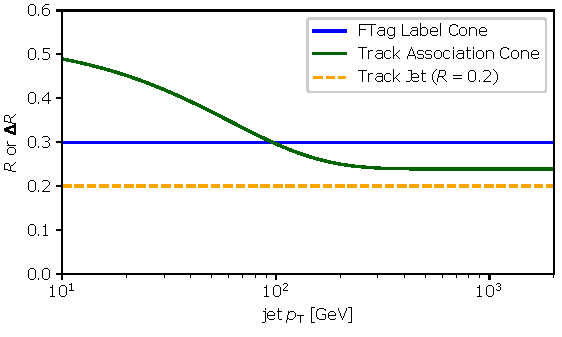
\includegraphics[width=0.5\textwidth]{shrinkCone}
  \caption{The shrinking particle association cone (\hexline{006401}) used to associate muons with a $\DeltaR_\mathrm{\mu, jet}$ smaller than the cone depending on the transverse momentum of the jet. Adopted from \citep{Jacobs:2697316}. }
  \label{fig:shrinkCone}
\end{figure}
Selected muons must be combined muons meaning they are reconstructed using both the inner detector and the muon spectrometer. The closest muon within $\DeltaR_\mathrm{\mu, jet} < 0.4$ to the jet axis is chosen provided it has a minimum \pt of \qty{4}{GeV}. This threshold is set as muon reconstruction below \qty{3}{GeV} is generally unreliable due to minimally ionizing particles losing approximately \qty{3}{GeV} in the ATLAS calorimeters \citep{expectedPerformanceAtlas}.

Truth studies revealed that most muons associated to jets result from secondary (non-prompt) decays of $c$- and $b$-hadrons as evidenced in figure \ref{fig:muonTruth}(a). However this figure also reveals the introduction of $b$-tagging backgrounds since muons are also associated to light jets. These backgrounds predominantly arise from in flight decays of pions and kaons but also prompt muons from nearby $W$-boson decays and muons from light and strange mesons as shown in figure \ref{fig:muonTruth}(b).
\begin{figure}[]
  \centering
  \subfigure[]{
    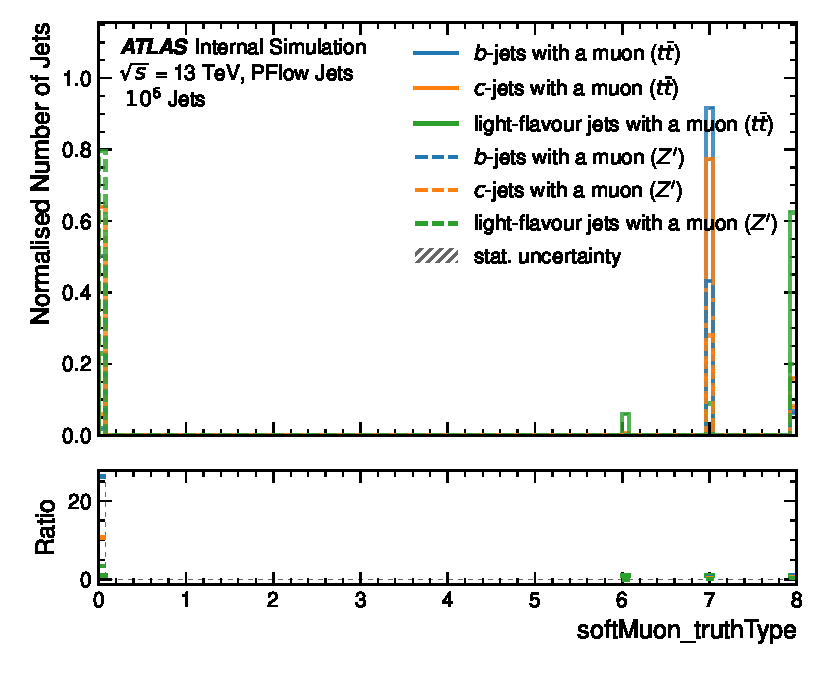
\includegraphics[width=0.47\textwidth]{softMuon_truthType_norm}
  }
  \subfigure[]{
    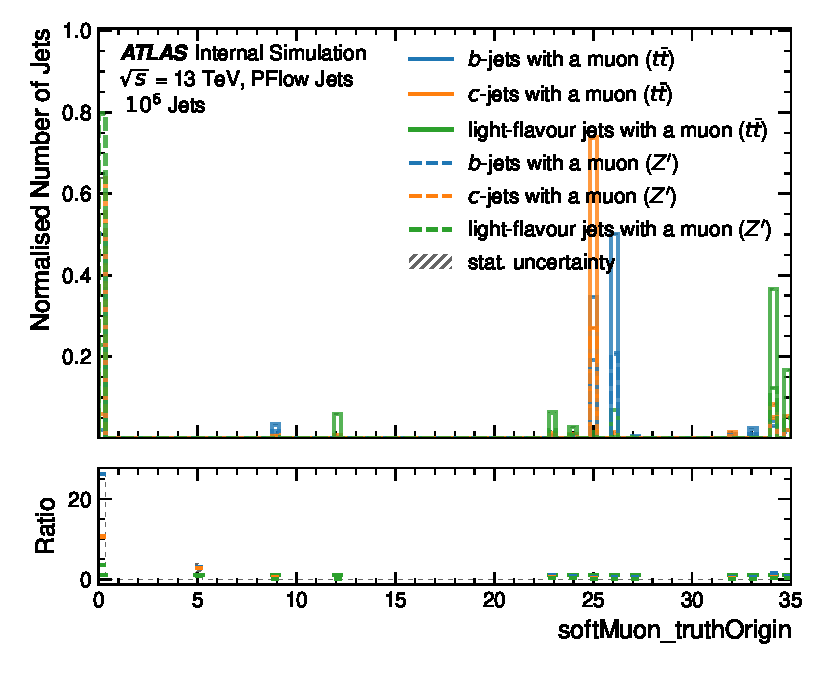
\includegraphics[width=0.47\textwidth]{softMuon_truthOrigin_norm}
  }
  \caption{Jet truth type (a) and truth origin (b) for jets with an associated muon normalized per flavor from $t\overline{t}$ and $Z'$ samples. Truth types: unclassified (0), prompt (6), non-prompt (7) and background muon (8). Truth origins: tau lepton decays (9), prompt muons from nearby W decays (12), light (23), strange (24), charm (25), bottom (26) mesons and in flight decays of pions (34) and kaons (35) according to the Monte Carlo truth classification \citep{mctruthclassification}.}
  \label{fig:muonTruth}
\end{figure}
Table \ref{tab:MuonJetFlavors} shows the proportion of jets with an associated muon for each flavor. Approximately \qty{15}{\percent} of $b$-jets and around \qty{1}{\percent} of both light and tau jets have an associated muon.
\begin{table}[]
  \caption{Fraction of associated muons per flavor. The large fraction for $b$-jets compared to the other flavors is the reason why muons are a useful discriminator for $b$-tagging. }
  \label{tab:MuonJetFlavors}
  \centering
  \begin{tabular}{ l c }
    \hline
    Jet flavor & Fraction of jets with an associated muon \\
    \hline
    light      & 0.0134                                   \\
    c          & 0.0472                                   \\
    b          & 0.1490                                   \\
    tau        & 0.0138                                   \\
    \hline
  \end{tabular}
\end{table}
Figure \ref{fig:muon_2d_truth} visualizes the amount of fake muons in $b$-jets with an associated muons depending on the jet- and muon-\pt. A notable trend is that $b$-jets with low momentum tend to have low momentum muons. Falsely associated muons become more common at high jet momentum and low muon momentum.
\begin{figure}[]
  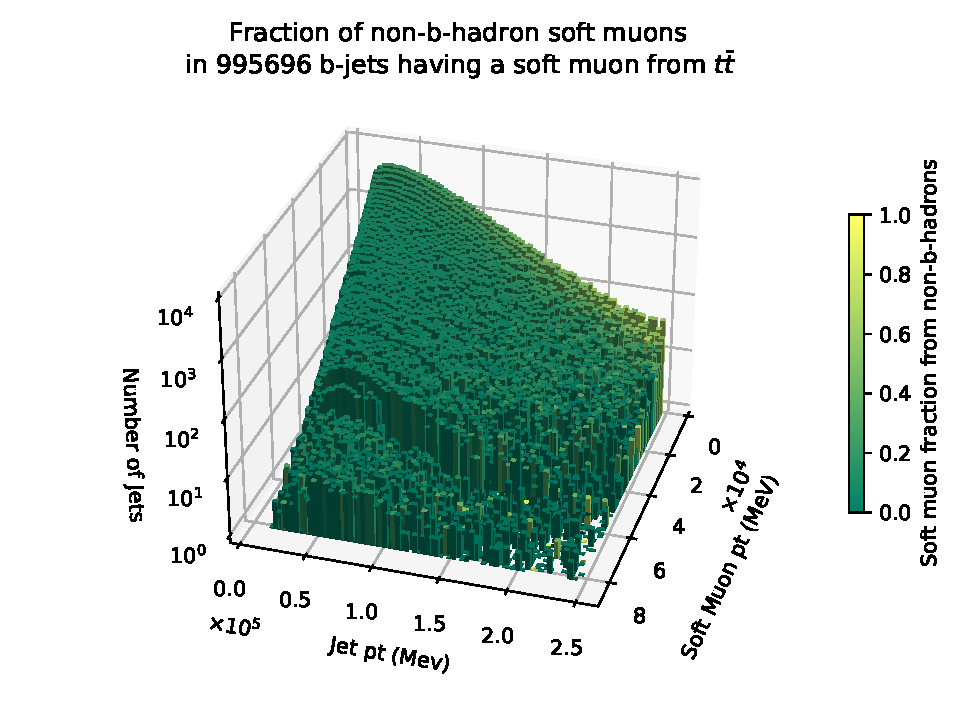
\includegraphics[width=1\textwidth]{muon_2d_truth_ttbar}
  \caption{2D histograms of $p_\mathrm{T}^\mathrm{jet}$ and $p_\mathrm{T}^\mathrm{muon}$ for $b$-jets with an associated muons from a $t\bar{t}$ sample. The colorbar is the fraction of muons that do not originate from b-hadrons. Irregularities in the distribution are due to a bug in the plotting library.}
  \label{fig:muon_2d_truth}
\end{figure}



\section{Soft Muon Variables}
\label{sec:SoftMuonVariables}
The soft muon variables are selected based on their $b$-tagging discrimination power. The impact parameters of jets as described in section \ref{sec:b_tagging} are determined with the three dimensional impact parameter algorithm (IP3D) detailed in \citep{ATL-PHYS-PUB-2017-013} and are shown in figure \ref{fig:softMuon_ip3dD0}-\ref{fig:softMuon_ip3dZ0Significance}.
\begin{figure}[]
  \centering
  \subfigure[]{
    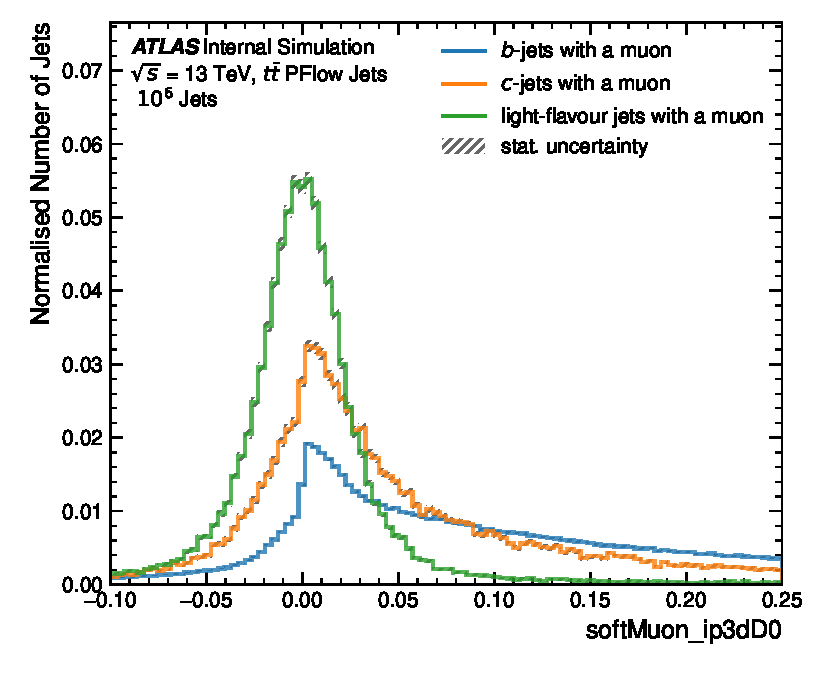
\includegraphics[width=0.47\textwidth]{softMuon_ip3dD0}
    \label{fig:softMuon_ip3dD0}
  }
  \subfigure[]{
    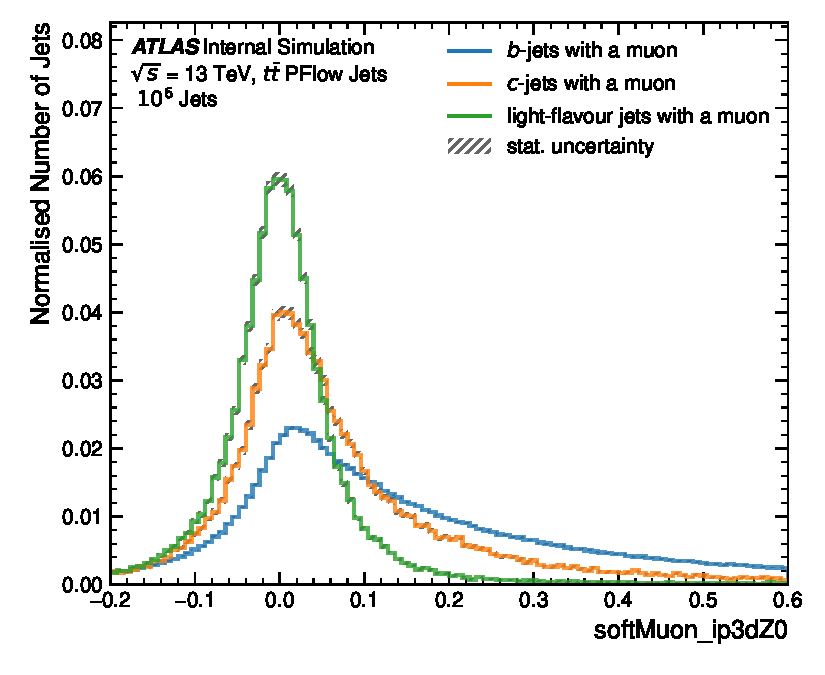
\includegraphics[width=0.47\textwidth]{softMuon_ip3dZ0}
    \label{fig:softMuon_ip3dZ0}
  }
  \\
  \subfigure[]{
    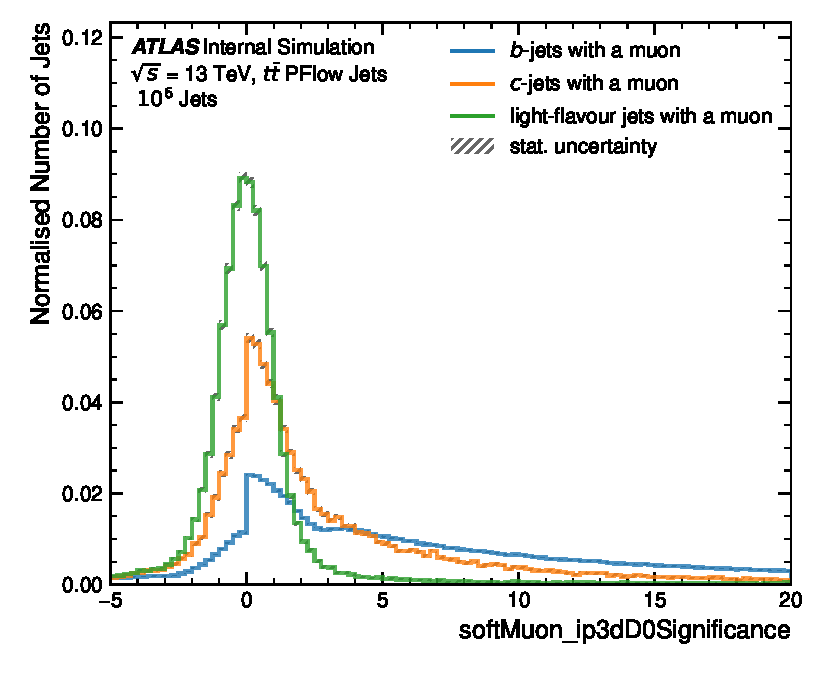
\includegraphics[width=0.47\textwidth]{softMuon_ip3dD0Significance}
    \label{fig:softMuon_ip3dD0Significance}
  }
  \subfigure[]{
    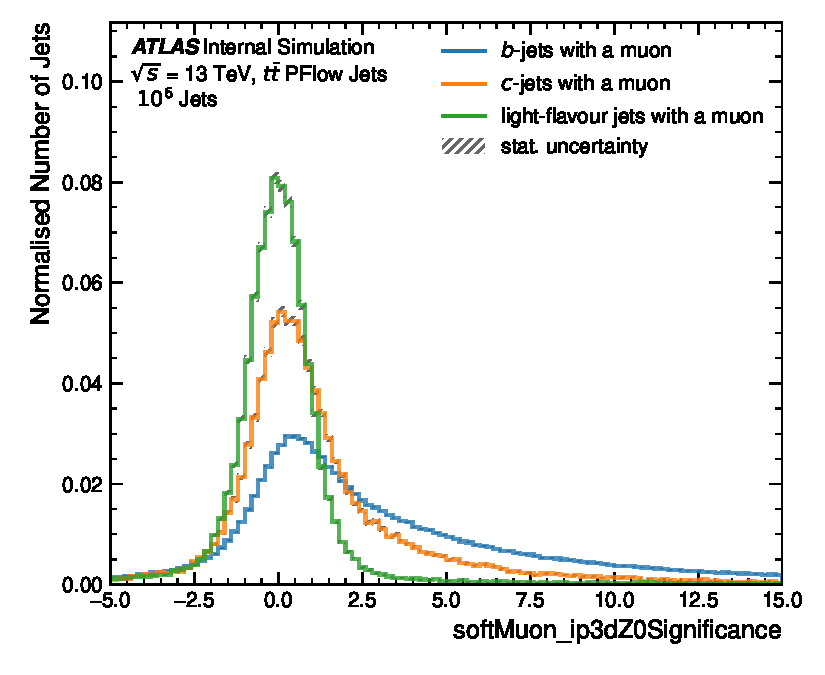
\includegraphics[width=0.47\textwidth]{softMuon_ip3dZ0Significance}
    \label{fig:softMuon_ip3dZ0Significance}
  }
  \caption{Impact parameters of the soft muon retrieved with the IP3D algorithm \citep{ATL-PHYS-PUB-2017-013}.}
  \label{fig:softMuonKinematics}
\end{figure}
In addition variables are used to reject muons from in flight decays of Kaons and Pions \citep{ATLAS-CONF-2020-030}. The Scattering Neighbor Significance measures if the track of a particle has kinks that could be a sign of an additional decay. By connecting neighboring detector hits along the track with straight lines and measuring the angles between adjacent lines the Scattering Neighbor Significance is obtained by taking the maximum of the angle divided by its uncertainty. In figure \ref{fig:softMuon_scatteringNeighbourSignificance} light jets therefore tend to have larger values as they have a smaller \pt (cf. figure \ref{fig:softMuon_pt}). Another variable to identify possible background sources is the Momentum Balance Significance. It calculates the difference of the muon-\pt determined with the inner detector with the one from the muon spectrometer and corrects it for energy deposits in the calorimeters. This would be zero in figure \ref{fig:softMuon_momentumBalanceSignificance} for a perfect energy loss correction and if the muon did not arise from an in flight decay. Furthermore there is the curvature comparison between inner detector (ID) and the one from the muon spectrometer (MS) termed q over p ratio: $(q/p)_\mathrm{ID}\, \bm{/}\, (q/p)_\mathrm{MS}$ in figure \ref{fig:softMuon_qOverPratio}.

\begin{figure}[]
  \centering
  \subfigure[]{
    \includegraphics[width=0.47\textwidth]{softMuon_scatteringNeighbourSignificance}
    \label{fig:softMuon_scatteringNeighbourSignificance}
  }
  \subfigure[]{
    \includegraphics[width=0.47\textwidth]{softMuon_momentumBalanceSignificance}
    \label{fig:softMuon_momentumBalanceSignificance}
  }
  \\
  \subfigure[]{
    \includegraphics[width=0.47\textwidth]{softMuon_qOverPratio}
    \label{fig:softMuon_qOverPratio}
  }
  \caption{Variables designed to reject light jet backgrounds. Description in section \ref{sec:SoftMuonVariables}.}
  \label{fig:softMuonVariables2}
\end{figure}


\section{Neural Network Training}
For all trainings the Umami neural network training framework \citep{Froch:2857164} is used with \ttbar and \Zprime Monte Carlo samples described in \citep{ATL-PHYS-PUB-2017-013}. \Zprime is a hypothetical particle used here to enhance the statistics at larger jet-\pt$>\SI{250}{GeV}$. For the training both \ttbar and \Zprime samples are merged and resampled to make the \pt and $\eta$ distributions appear the same for all flavors. This is done to allow for a fair \ac{nn} training between flavor categories, as the kinematic regimes are neither over- nor under-represented between flavors. The flavor composition of jets can be seen before and after applying the resampling in figure \ref{fig:resampling}. A total of \qty{23.6e6}{} jets are used with \qty{3.9e6}{} jets (\qty{16.6}{\percent}) having an associated soft muon.
\begin{figure}
  \centering
  \subfigure[]{\includegraphics[width=.8\textwidth]{pt_btagJes-cut_spectrum}}\\
  \subfigure[]{\includegraphics[width=.8\textwidth]{pt_btagJes-downsampled}}
  \caption[]{Jet-\pt per flavor normalized to unity for \ttbar and \Zprime samples \textbf{(a)} before and \textbf{(b)} after resampling. Adopted from \citep{umamiDocs}.}
  \label{fig:resampling}
\end{figure}


\section{Adding muons to $b$-tagging algorithms}\label{sec:add_muons}
Current $b$-tagging algorithms in use are deep feed-forward neural networks with the prefix \ac{dl1} that assign a probability score ($p_\mathrm{b}, p_\mathrm{c}, p_\mathrm{light}$) to a jet depending on its flavor content. Depending on the strategy used to introduce additional tracking information associated with the jet \ac{dl1} can become DL1r if the outputs of the RNNIP (Recurrent Neural Network Impact Parameter) \citep{Gilles:2806947} tagger or DL1d if the outputs of the \ac{dips} \citep{ATL-PHYS-PUB-2020-014} tagger are added as inputs to \ac{dl1}. The outputs of these taggers are then combined into a single signal to background ratio variable, the discriminant, defined as
\begin{equation}
  \mathrm{D}=\ln\left(\frac{p_b}{f_c \cdot p_c + (1-f_c)\cdot p_\mathrm{light} }\right).
\end{equation}
$f_c$ is the fraction of charm jets in the background and can be used to tune the importance of the different background classes ($\sum f_\mathrm{bkg} =1$). Figure \ref{fig:scores_comparison_DL1d_to_DL1dmu} illustrates the flavor distribution of this discriminant.
\begin{figure}[]
  \centering
  \includegraphics[width=0.7\textwidth]{scores_comparison_DL1d_to_DL1dmu}
  \caption{Discriminant comparison between DL1d ($\bm{\diagup$}) and DL1dmu (\textbf{- -}). Enhanced model performance is indicated by greater visual separation between the classes.}
  \label{fig:scores_comparison_DL1d_to_DL1dmu}
\end{figure}

The selected muon variables are added to DL1r/DL1d as additional inputs. For a performance reference point initial trainings of DL1r were conducted and two ways of introducing the muon information were explored. The first refers to an approach where the muon variables itself were used to train an additional neural network called the \ac{smt} with architecture: (soft muon input variables) $\rightarrow$ 3 hidden layers (100, 20, 10) $\rightarrow (p_\text{b}, p_\text{c}, p_\text{light})$. The output scores of the \ac{smt} are then added as inputs to the \ac{dl1} training. The tagger resulting from this method will be referred to as DL1rSMT. In a second approach the muon variables were added directly as inputs to the DL1r training and are denoted as DL1rmu.

\section{Performance evaluation}
A retraining of the DL1r or DL1d tagger serves in all cases as performance baseline against which other models are compared to. As a typical evaluation metric \ac{roc} curves are used to evaluate a classifier. In these curves the true positive rate (rate at which the classifier identifies correctly what it should identify) is plotted against the false positive rate (rate at which the classifier identifies falsely what it should identify). The first translates here into the $b$-jet efficiency. It corresponds to integrating from right to left in figure \ref{fig:scores_comparison_DL1d_to_DL1dmu} for a desired $b$-jet efficiency. The latter (false positive rate) will be plotted inversely here as rejection instead of as efficiency (1/$\epsilon_\mathrm{flavor}$). For the case at hand the performance increases if the curve moves to the upper right corner, as the model can reject more background for a designated $b$-jet efficiency. If the \ac{roc} curve of a classifier would be a \qty{45}{\degree} line the classifier is of no use as there would be always a \qty{50}{\percent} chance to correctly or falsely identify a property of interest, essentially performing no better than random chance.

\section{DL1rmu vs. DL1rSMT}
\ac{roc} curves comparing performances of DL1r, DL1rmu and DL1rSMT are shown in figure \ref{fig:DL1rmu_vs_DL1r_SMT_tt} and \ref{fig:DL1rmu_vs_DL1r_SMT_z} and display for both methods a \qty{25}{\percent} improvement in the light flavor jet rejection and a \qty{10}{\percent} $c$-flavor jet rejection upon introducing muon variables. Since adding the soft muon variables to the inputs of DL1r/DL1d results in fewer technical interdependencies and also allows DL1r to figure out potential correlations to other variables, it was decided to default to this option.

\begin{figure}[]
  \centering
  \subfigure[]{
    \includegraphics[width=0.477\textwidth]{DL1r_light_flavour_ttbar_229}
    \label{fig:DL1rmu_vs_DL1r_SMTa}
  }
  \subfigure[]{
    \includegraphics[width=0.477\textwidth]{DL1r_c_flavour_ttbar_229}
    \label{fig:DL1rmu_vs_DL1r_SMTb}
  }
  \caption{ROC curves of different trainings. Official performance of DL1r (\hexline{1F77B5}), Trainings: DL1r (\hexline{549F41}), DL1rmu (\hexline{EF8636}) adds the soft muon variables to the inputs variables of DL1r,  DL1rSMT (\hexline{C53A32}) adds the outputs from the standalone Soft Muon Tagger neural network to the inputs of DL1r evaluated on \ttbar. }
  \label{fig:DL1rmu_vs_DL1r_SMT_tt}
\end{figure}

\begin{figure}[]
  \centering
  \subfigure[]{
    \includegraphics[width=0.477\textwidth]{DL1r_light_flavour_zpext_229}
    \label{fig:DL1rmu_vs_DL1r_SMTc}
  }
  \subfigure[]{
    \includegraphics[width=0.477\textwidth]{DL1r_c_flavour_zpext_229}
    \label{fig:DL1rmu_vs_DL1r_SMTd}
  }
  \caption{ROC curves of different trainings. Official performance of DL1r (\hexline{1F77B5}), Trainings: DL1r (\hexline{549F41}), DL1rmu (\hexline{EF8636}) adds the soft muon variables to the inputs variables of DL1r,  DL1rSMT (\hexline{C53A32}) adds the outputs from the standalone Soft Muon Tagger neural network to the inputs of DL1r evaluated on \Zprime. }
  \label{fig:DL1rmu_vs_DL1r_SMT_z}
\end{figure}



\section{Additional soft muon variables}
The full potential of muons were explored phenomenologically by successively adding input variables of four different classes to \ac{dl1}. New inputs are categorized into variables related to quality criteria used by the \ac{mcp} group, number of hits in the various subdetectors of the inner detector and of course the tracking information from \ac{dips} and mentioned \ac{smt} variables as detailed in \ref{sec:SoftMuonVariables}.

The different variations of input variables are shown in table \ref{tab:smtAbbreviations} and \ref{tab:DL1dModels} while figures \ref{fig:smt_vars_1}-\ref{fig:smt_vars_7} show their distributions per flavor. Table \ref{tab:smtAbbreviations} is a reduced version of available variables since some of them did not display any flavor discrimination power. A detailed explanation and modeling of these variables can be found in \citep{Assamagan:1099953,Bugge:2665711}.

\begin{table}[]
  % \sisetup{group-minimum-digits=4}
  \caption{Abbreviations for the different sets of variables}%
  \label{tab:smtAbbreviations}
  \centering
  \resizebox{0.97\textwidth}{!}{
    \begin{tabular}{c|l|l
      }
      \hline
      Abbreviation                & SMT                              & Hits                                      \\
      \hline
      \multirow{15}{*}{Soft Muon} & \pt                              & numberOfInnermostPixelLayerHits           \\
                                  & \DeltaR                          & numberOfInnermostPixelLayerSplitHits      \\
                                  & q over p ratio                   & numberOfInnermostPixelLayerSharedHis      \\
                                  & Momentum Balance Significance    & numberOfInnermostPixelLayerOutliers       \\
                                  & Scattering Neighbor Significance & numberOfNextToInnermostPixelLayerHits     \\
                                  & \ptrel                           & numberOfNextToInnermostPixelLayerOutliers \\
                                  & ip3dD0                           & numberOfPixelHits                         \\
                                  & ip3dZ0                           & numberOfPixelSplitHits                    \\
      Variables                   & ip3dD0 Significance              & numberOfPixelSharedHits                   \\
                                  & ip3dZ0 Significance              & numberOfPixelSpoiltHits                   \\
                                  & isDefaults                       & numberOfPixelHoles                        \\
                                  &                                  & numberOfSCTHits                           \\
                                  &                                  & numberOfSCTSharedHits                     \\
                                  &                                  & numberOfSCTHoles                          \\
                                  &                                  & expectInnermostPixelLayerHits             \\
                                  &                                  & expectNextToInnermostPixelLayerHits       \\

      \hline
      Abbreviation                & MCP                              & dips                                      \\
      \hline
      \multirow{9}{*}{Soft Muon}  & segmentDeltaEta                  & dipsLoose20210729 pb                      \\
                                  & segmentDeltaPhi                  & dipsLoose20210729 pc                      \\
                                  & ParamEnergyLoss                  & dipsLoose20210729 pu                      \\
                                  & ParamEnergyLossSigmaPlus         &                                           \\
                                  & ParamEnergyLossSigmaMinus        &                                           \\
      Variables                   & MeasEnergyLoss                   &                                           \\
                                  & MeasEnergyLossSigma              &                                           \\
                                  & CaloMuonScore                    &                                           \\
                                  & Muon Quality                     &                                           \\
                                  & Nr. of Associated Muons          &                                           \\
                                  & CaloMuonIDTag                    &                                           \\
      \hline
    \end{tabular}
  }
\end{table}

\begin{table}[]
  % \sisetup{group-minimum-digits=4}
  \caption{Variables used in the different trainings of DL1d}%
  \label{tab:DL1dModels}
  \centering

  \begin{tabular}{c| llll
    }
    \hline
    Model                            & DL1d & DL1dmu & DL1dmu add hits & DL1dmu add all \\
    \hline
    \multirow{4}{*}{Input Variables} & DL1  & DL1    & DL1             & DL1            \\
                                     & dips & dips   & dips            & dips           \\
                                     &      & SMT    & SMT             & SMT            \\
                                     &      &        & Hits            & Hits           \\
                                     &      &        &                 & MCP            \\
    \hline
  \end{tabular}
\end{table}

\newcommand\plotsize{0.30}
\begin{figure}[]
    \centering
    \subfigure[]{
        \includegraphics[width=\plotsize\textwidth]{input_vars_smt_ttbar_zpext/softMuon_pt}
    }
    \subfigure[]{
        \includegraphics[width=\plotsize\textwidth]{input_vars_smt_ttbar_zpext/softMuon_dR}
    }
    \subfigure[]{
        \includegraphics[width=\plotsize\textwidth]{input_vars_smt_ttbar_zpext/softMuon_eta}
    }\\
    \subfigure[]{
        \includegraphics[width=\plotsize\textwidth]{input_vars_smt_ttbar_zpext/softMuon_phi}
    }
    \subfigure[]{
        \includegraphics[width=\plotsize\textwidth]{input_vars_smt_ttbar_zpext/softMuon_qOverPratio}
    }
    \subfigure[]{
        \includegraphics[width=\plotsize\textwidth]{input_vars_smt_ttbar_zpext/softMuon_momentumBalanceSignificance}
    }\\
    \subfigure[]{
        \includegraphics[width=\plotsize\textwidth]{input_vars_smt_ttbar_zpext/softMuon_scatteringNeighbourSignificance}
    }
    \subfigure[]{
        \includegraphics[width=\plotsize\textwidth]{input_vars_smt_ttbar_zpext/softMuon_pTrel}
    }
    \subfigure[]{
        \includegraphics[width=\plotsize\textwidth]{input_vars_smt_ttbar_zpext/softMuon_ip3dD0}
    }\\
    \subfigure[]{
        \includegraphics[width=\plotsize\textwidth]{input_vars_smt_ttbar_zpext/softMuon_ip3dZ0}
    }
    \subfigure[]{
        \includegraphics[width=\plotsize\textwidth]{input_vars_smt_ttbar_zpext/softMuon_ip3dD0Significance}
    }
    \subfigure[]{
        \includegraphics[width=\plotsize\textwidth]{input_vars_smt_ttbar_zpext/softMuon_ip3dZ0Significance}
    }
    \caption{Explored muon variables (1/7)}
    \label{fig:smt_vars_1}
\end{figure}








\begin{figure}[]
    \centering
    \subfigure[]{
        \includegraphics[width=\plotsize\textwidth]{input_vars_smt_ttbar_zpext/softMuon_isDefaults}
    }
    \subfigure[]{
        \includegraphics[width=\plotsize\textwidth]{input_vars_smt_ttbar_zpext/softMuon_ip3dD0Uncertainty}
    }
    \subfigure[]{
        \includegraphics[width=\plotsize\textwidth]{input_vars_smt_ttbar_zpext/softMuon_ip3dZ0Uncertainty}
    }\\
    \subfigure[]{
        \includegraphics[width=\plotsize\textwidth]{input_vars_smt_ttbar_zpext/softMuon_dr_closest_reco_lepton}
    }
    \subfigure[]{
        \includegraphics[width=\plotsize\textwidth]{input_vars_smt_ttbar_zpext/softMuon_dr_closest_prompt_truth_lepton}
    }
    \subfigure[]{
        \includegraphics[width=\plotsize\textwidth]{input_vars_smt_ttbar_zpext/softMuon_dr_closest_non_prompt_truth_lepton}
    }\\
    \subfigure[]{
        \includegraphics[width=\plotsize\textwidth]{input_vars_smt_ttbar_zpext/softMuon_truthOrigin}
    }
    \subfigure[]{
        \includegraphics[width=\plotsize\textwidth]{input_vars_smt_ttbar_zpext/softMuon_truthType}
    }
    \subfigure[]{
        \includegraphics[width=\plotsize\textwidth]{input_vars_smt_ttbar_zpext/softMuon_nr_truth_muons_in_max_dr}
    }\\
    \subfigure[]{
        \includegraphics[width=\plotsize\textwidth]{input_vars_smt_ttbar_zpext/softMuon_nr_reco_muons_in_max_dr}
    }
    \subfigure[]{
        \includegraphics[width=\plotsize\textwidth]{input_vars_smt_ttbar_zpext/softMuon_nr_prompt_leptons}
    }
    \subfigure[]{
        \includegraphics[width=\plotsize\textwidth]{input_vars_smt_ttbar_zpext/softMuon_nr_non_prompt_leptons}
    }
    \caption{Explored muon variables (2/7)}
    \label{fig:smt_vars_2}
\end{figure}







\begin{figure}[]
    \centering
    \subfigure[]{
        \includegraphics[width=\plotsize\textwidth]{input_vars_smt_ttbar_zpext/softMuon_quality}
    }
    \subfigure[]{
        \includegraphics[width=\plotsize\textwidth]{input_vars_smt_ttbar_zpext/softMuon_passed_lowPT_counter}
    }
    \subfigure[]{
        \includegraphics[width=\plotsize\textwidth]{input_vars_smt_ttbar_zpext/softMuon_isLowPT}
    }\\
    \subfigure[]{
        \includegraphics[width=\plotsize\textwidth]{input_vars_smt_ttbar_zpext/muon_scatteringCurvatureSignificance}
    }
    \subfigure[]{
        \includegraphics[width=\plotsize\textwidth]{input_vars_smt_ttbar_zpext/muon_spectrometerFieldIntegral}
    }
    \subfigure[]{
        \includegraphics[width=\plotsize\textwidth]{input_vars_smt_ttbar_zpext/muon_segmentDeltaEta}
    }\\
    \subfigure[]{
        \includegraphics[width=\plotsize\textwidth]{input_vars_smt_ttbar_zpext/muon_segmentDeltaPhi}
    }
    \subfigure[]{
        \includegraphics[width=\plotsize\textwidth]{input_vars_smt_ttbar_zpext/muon_segmentChi2OverDoF}
    }
    \subfigure[]{
        \includegraphics[width=\plotsize\textwidth]{input_vars_smt_ttbar_zpext/muon_t0}
    }\\
    \subfigure[]{
        \includegraphics[width=\plotsize\textwidth]{input_vars_smt_ttbar_zpext/muon_beta}
    }
    \subfigure[]{
        \includegraphics[width=\plotsize\textwidth]{input_vars_smt_ttbar_zpext/muon_annBarrel}
    }
    \subfigure[]{
        \includegraphics[width=\plotsize\textwidth]{input_vars_smt_ttbar_zpext/muon_annEndCap}
    }
    \caption{Explored muon variables (3/7)}
    \label{fig:smt_vars_3}
\end{figure}




\begin{figure}[]
    \centering
    \subfigure[]{
        \includegraphics[width=\plotsize\textwidth]{input_vars_smt_ttbar_zpext/muon_innAngle}
    }
    \subfigure[]{
        \includegraphics[width=\plotsize\textwidth]{input_vars_smt_ttbar_zpext/muon_midAngle}
    }
    \subfigure[]{
        \includegraphics[width=\plotsize\textwidth]{input_vars_smt_ttbar_zpext/muon_msInnerMatchChi2}
    }\\
    \subfigure[]{
        \includegraphics[width=\plotsize\textwidth]{input_vars_smt_ttbar_zpext/muon_msOuterMatchChi2}
    }
    \subfigure[]{
        \includegraphics[width=\plotsize\textwidth]{input_vars_smt_ttbar_zpext/muon_meanDeltaADCCountsMDT}
    }
    \subfigure[]{
        \includegraphics[width=\plotsize\textwidth]{input_vars_smt_ttbar_zpext/muon_CaloLRLikelihood}
    }\\
    \subfigure[]{
        \includegraphics[width=\plotsize\textwidth]{input_vars_smt_ttbar_zpext/muon_FSR_CandidateEnergy}
    }
    \subfigure[]{
        \includegraphics[width=\plotsize\textwidth]{input_vars_smt_ttbar_zpext/muon_EnergyLoss}
    }
    \subfigure[]{
        \includegraphics[width=\plotsize\textwidth]{input_vars_smt_ttbar_zpext/muon_ParamEnergyLoss}
    }\\
    \subfigure[]{
        \includegraphics[width=\plotsize\textwidth]{input_vars_smt_ttbar_zpext/muon_MeasEnergyLoss}
    }
    \subfigure[]{
        \includegraphics[width=\plotsize\textwidth]{input_vars_smt_ttbar_zpext/muon_EnergyLossSigma}
    }
    \subfigure[]{
        \includegraphics[width=\plotsize\textwidth]{input_vars_smt_ttbar_zpext/muon_ParamEnergyLossSigmaPlus}
    }
    \caption{Explored muon variables (4/7)}
    \label{fig:smt_vars_4}
\end{figure}



\begin{figure}[]
    \centering

    \subfigure[]{
        \includegraphics[width=\plotsize\textwidth]{input_vars_smt_ttbar_zpext/muon_ParamEnergyLossSigmaMinus}
    }
    \subfigure[]{
        \includegraphics[width=\plotsize\textwidth]{input_vars_smt_ttbar_zpext/muon_MeasEnergyLossSigma}
    }
    \subfigure[]{
        \includegraphics[width=\plotsize\textwidth]{input_vars_smt_ttbar_zpext/muon_CaloMuonScore}
    }\\
    \subfigure[]{
        \includegraphics[width=\plotsize\textwidth]{input_vars_smt_ttbar_zpext/muon_msInnerMatchDOF}
    }
    \subfigure[]{
        \includegraphics[width=\plotsize\textwidth]{input_vars_smt_ttbar_zpext/muon_msOuterMatchDOF}
    }
    \subfigure[]{
        \includegraphics[width=\plotsize\textwidth]{input_vars_smt_ttbar_zpext/muon_CaloMuonIDTag}
    }\\
    \subfigure[]{
        \includegraphics[width=\plotsize\textwidth]{input_vars_smt_ttbar_zpext/softMuon_numberOfPixelHits}
    }
    \subfigure[]{
        \includegraphics[width=\plotsize\textwidth]{input_vars_smt_ttbar_zpext/softMuon_numberOfPixelSharedHits}
    }
    \subfigure[]{
        \includegraphics[width=\plotsize\textwidth]{input_vars_smt_ttbar_zpext/softMuon_numberOfSCTHits}
    }\\
    \subfigure[]{
        \includegraphics[width=\plotsize\textwidth]{input_vars_smt_ttbar_zpext/softMuon_numberOfSCTSharedHits}
    }
    \subfigure[]{
        \includegraphics[width=\plotsize\textwidth]{input_vars_smt_ttbar_zpext/softMuon_numberOfNextToInnermostPixelLayerHits}
    }
    \subfigure[]{
        \includegraphics[width=\plotsize\textwidth]{input_vars_smt_ttbar_zpext/softMuon_numberOfInnermostPixelLayerHits}
    }
    \caption{Explored muon variables (5/7)}
    \label{fig:smt_vars_5}
\end{figure}


\begin{figure}[]
    \centering

    \subfigure[]{
        \includegraphics[width=\plotsize\textwidth]{input_vars_smt_ttbar_zpext/softMuon_numberOfInnermostPixelLayerSharedHits}
    }
    \subfigure[]{
        \includegraphics[width=\plotsize\textwidth]{input_vars_smt_ttbar_zpext/softMuon_numberOfInnermostPixelLayerSplitHits}
    }
    \subfigure[]{
        \includegraphics[width=\plotsize\textwidth]{input_vars_smt_ttbar_zpext/softMuon_numberOfPixelSplitHits}
    }\\
    \subfigure[]{
        \includegraphics[width=\plotsize\textwidth]{input_vars_smt_ttbar_zpext/softMuon_numberOfUsedHitsdEdx}
    }
    \subfigure[]{
        \includegraphics[width=\plotsize\textwidth]{input_vars_smt_ttbar_zpext/softMuon_numberOfNextToInnermostPixelLayerSharedHits}
    }
    \subfigure[]{
        \includegraphics[width=\plotsize\textwidth]{input_vars_smt_ttbar_zpext/softMuon_numberOfNextToInnermostPixelLayerSplitHits}
    }\\
    \subfigure[]{
        \includegraphics[width=\plotsize\textwidth]{input_vars_smt_ttbar_zpext/softMuon_numberOfPixelSpoiltHits}
    }
    \subfigure[]{
        \includegraphics[width=\plotsize\textwidth]{input_vars_smt_ttbar_zpext/softMuon_numberOfDBMHits}
    }
    \subfigure[]{
        \includegraphics[width=\plotsize\textwidth]{input_vars_smt_ttbar_zpext/softMuon_numberOfSCTSpoiltHits}
    }\\
    \subfigure[]{
        \includegraphics[width=\plotsize\textwidth]{input_vars_smt_ttbar_zpext/softMuon_numberOfTRTHits}
    }
    \subfigure[]{
        \includegraphics[width=\plotsize\textwidth]{input_vars_smt_ttbar_zpext/softMuon_numberOfTRTHighThresholdHits}
    }
    \subfigure[]{
        \includegraphics[width=\plotsize\textwidth]{input_vars_smt_ttbar_zpext/softMuon_numberOfTRTHighThresholdHitsTotal}
    }
    \caption{Explored muon variables (6/7)}
    \label{fig:smt_vars_6}
\end{figure}

\begin{figure}[]
    \centering


    \subfigure[]{
        \includegraphics[width=\plotsize\textwidth]{input_vars_smt_ttbar_zpext/softMuon_numberOfTRTTubeHits}
    }
    \subfigure[]{
        \includegraphics[width=\plotsize\textwidth]{input_vars_smt_ttbar_zpext/softMuon_numberOfTRTXenonHits}
    }
    \subfigure[]{
        \includegraphics[width=\plotsize\textwidth]{input_vars_smt_ttbar_zpext/softMuon_numberOfTRTSharedHits}
    }\\
    \subfigure[]{
        \includegraphics[width=\plotsize\textwidth]{input_vars_smt_ttbar_zpext/softMuon_TRTdEdxUsedHits}
    }
    
    \caption{Explored muon variables (7/7)}
    \label{fig:smt_vars_7}
\end{figure}

\section{Adding a muon quality criterion}
Muons used in the association are as inclusive as possible and therefore apart from the selection mentioned in section \ref{sec:MuonSelection} no further quality criterion were applied initially. In other trainings muons were required to have the  ``low pt'' muon identification working point \citep{ATL-PHYS-PUB-2020-002}. This quality criterion improves the muon selection efficiency for muons in the range particularly relevant for this study $\qty[]{3}{GeV}<\pt < \qty[]{6}{GeV}$ (cf. figure \ref{fig:softMuon_pt}). It reduces the backgrounds by \qty{54}{\percent} for light flavor jets and by \qty{23}{\percent} for tau-jets by keeping \qty{77}{\percent} of the $c$-jets and \qty{90}{\percent} of the $b$-jets (cf. table \ref{tab:lowPtMuonJetFlavors}).
\begin{table}[]
  % \sisetup{group-minimum-digits=4}
  \caption{Fraction of associated low pt working point muons per flavor. Fraction of low pt muons to all associated muons (fractions to table \ref{tab:MuonJetFlavors}), the fraction of muons kept after applying the working point. }%
  \label{tab:lowPtMuonJetFlavors}
  \centering
  \resizebox{0.97\textwidth}{!}{
    \begin{tabular}{%
        l
        c
        c
      }
      \hline
      {Jet flavor} & {Fraction of jets with an associated low pt muon} & Fraction of low pt muons \\
      \hline
      light        & 0.0062                                            & 0.4626                   \\
      c            & 0.0363                                            & 0.7690                   \\
      b            & 0.1338                                            & 0.8979                   \\
      tau          & 0.0096                                            & 0.6956                   \\
      \hline
    \end{tabular}}
\end{table}
One way to introduce this information into the neural network is to add another Boolean input variable \textit{isLowPt} that indicates whether the muon meets the necessary requirements for the identification working point. Another option is to use only the muons that passed the identification working point. Both methods were tested in separate trainings.

\section{Performance comparison to DL1d}
The various additions of muon information to different trainings of \ac{dl1} is evaluated in figure \ref{fig:DL1dmu_ttbar} and \ref{fig:DL1dmu_zpext}. DL1dmu shows similar to DL1r a \qty{25}{\percent} improvement in the light flavor jet rejection and a \qty{10}{\percent} $c$-flavor jet rejection but does neither improve significantly upon adding the hits variables nor for adding the parameters from the muon combined performance variables. Notably, when the ``lowPt'' identification working point is applied, DL1dmu shows further improvement in its rejection capabilities. Specifically, there's an additional increase of approximately $\sim$\qty{10}{\percent} in rejecting light flavor jets and about $\sim$\SI{5}{\percent} in rejecting $c$-flavor jets.

This is regardless if the more inclusive muon selection is used, where only the boolean \textit{lowPt} information is added as a variable or by using the \textit{lowPt} selected muons only which removes a notable \qty{44}{\percent} of the muons. This means that the neural network does not learn anything from the background muons, and that having a muon associated with a $b$-jet is the strongest indicator for a b-hadron. Hence, DL1dmu with the \textit{islowPt} variable, improves light flavor rejection by $\sim$\qty{40}{\percent} and c-flavor rejection by $\sim$\qty{30}{\percent} compared to the nominal DL1d training.

\begin{figure}[]
  \centering
  \includegraphics[width=1\textwidth]{DL1dmu_ttbar}
  \caption{ROC curves of studied models with reference to a trained DL1d model evaluated on \ttbar.}
  \label{fig:DL1dmu_ttbar}
\end{figure}
\begin{figure}[]
  \centering
  \includegraphics[width=1\textwidth]{DL1dmu_zpext}
  \caption{ROC curves of studied models with reference to a trained DL1d model evaluated on \Zprime.}
  \label{fig:DL1dmu_zpext}
\end{figure}

\section{Feature importance}
To understand the influence of a variable to a training of a neural network it can be evaluated with a framework called \ac{shap} \citep{shap,NIPS2017_7062}. It is based on the idea to turn input features on and off and to compare the \ac{ml} model's prediction for both cases. If this is done for all possible combinations the average impact a feature for a machine learning model can be estimated with the \ac{shap} value. Large positive or negative \ac{shap} values are thus indicators how significantly a particular input feature influences the model's prediction. In the context of $b$-tagging large negative \ac{shap} values will help the model to better reject whereas features with large positive \ac{shap} values helps the model to learn that these are most probably jets from a \ac{nn} output node of interest.

The evaluation for DL1dmu, with the boolean \textit{isLowPt} variable added, is shown in fig. \ref{fig:shapleyDL1dmu}. It clearly shows that main improvements over the previous implementation are due to the addition of the muon \pt and the low pt working point information to DL1dmu.
\begin{figure}[]
  \centering
  \includegraphics[width=1\textwidth]{ttbar_r22_shapley_b-jets}
  \caption{SHAP values for the $b$-jet output node of DL1dmu representing the impact of an input features influence to the neural network.}
  \label{fig:shapleyDL1dmu}
\end{figure}
The evaluation for the model that added all variables is shown in fig. \ref{fig:ttbar_r22_shapley_b_all_vars}. Even though a lot of the \ac{mcp} variables (see table \ref{tab:DL1dModels}) rank mediocre there was basically no improvement in performance (figure \ref{fig:DL1dmu_ttbar}-\ref{fig:DL1dmu_zpext}).
\begin{figure}[]
  \centering
  \includegraphics[width=0.97\textwidth]{ttbar_r22_shapley_b-jets_all_vars}
  \caption{SHAP values for the $b$-jet output node of the DL1dmu\_all\_vars representing the impact of an input features influence to the neural network.}
  \label{fig:ttbar_r22_shapley_b_all_vars}
\end{figure}
The minimal impact of incorporating most MCP variables on the model's performance is likely due to their strong linear correlation with the muon's transverse momentum. This correlation is clearly evident in the correlation matrix presented in Figure \ref{fig:correlation_matrix}. Since the \pt of the muon is already informatively represented in other variables, such as the Momentum Balance Significance, the additional MCP variables do not contribute significant new information to the model. A more detailed visual representation is shown in scatter plots of Figure \ref{fig:scatterplot_matrix_mcp} showcasing the relationships among \ac{smt} and \ac{mcp} variables.
\begin{figure}[]
  \centering
  \includegraphics[width=1\textwidth]{correlation_matrix}
  \caption{Linear correlations between all explored soft muon variables. E.g. \pt is strongly correlated to ParamEnergyLossSigmaPlus, which in turn is  correlated to ParamEnergyLoss. }
  \label{fig:correlation_matrix}
\end{figure}

\begin{figure}[]
  \centering
  \includegraphics[width=1\textwidth]{scatterplot_matrix_mcp}
  \caption{\ac{smt} and \ac{mcp} variables (see table \ref{tab:smtAbbreviations}) plotted against each other to reveal correlations. Overlays represent one standard deviation scattered points.}
  \label{fig:scatterplot_matrix_mcp}
\end{figure}

% VIVA_13.05.22.pdf ! 


\chapter{$HH\rightarrow 4b$ Results}\label{ch:hh4b-results}

This chapter presents the extracted cross-section limits for the $HH\rightarrow 4b$ analysis. 
\red{lets move the lin combine to the methodology part}
To test on any \ktwov hypothesis a linear combination of available samples is employed as explained and validated in \ref{sec:linear_combination}.The approach is employed bin-wise as the extraction factors deviate substantially per bin as shown in figure \ref{fig:linear_combine_bin_solutions}.
\begin{figure}
    \centering
    \includegraphics[width=.47\textwidth]{linear_combine_bin_solutions}
    \caption[]{Extracted reweighting factors for \red {equation blah} per bin.}
    \label{fig:linear_combine_bin_solutions}
\end{figure}
The method is validated with a $\ktwov=0$ sample for which also the nominally mc generated sample exists. Figure \ref{fig:tomatos_cls_5_nominal_reweighted_ratio} reveals a \qty[]{5}{\percent} deviation for this approach. \red{should one introduce a very conservative uncertainty because of that? the behavior across all values however is unclear with just one validation sample, maybe something for the outlook. } 
\begin{figure}
    \centering
    \includegraphics[width=.6\textwidth]{tomatos_cls_5_nominal_reweighted_ratio}
    \caption[]{Comparison between a \ac{mc}-generated $\ktwov=0$ signal sample and a signal sample created with the reweighting approach by linearly combining different \ktwov hypotheses. \red{whats with the mc stat error in general for the reweighted, makes stat err small as taken and scaled in my code from k2v=0}}
    \label{fig:tomatos_cls_5_nominal_reweighted_ratio}
\end{figure}


\begin{landscape}
    \begin{figure}
        \centering
        \subfigure[]{\includegraphics[width=.7\textwidth]{k2v_scan_limits_overlay_vbf_cut}}
        \subfigure[]{\includegraphics[width=.7\textwidth]{k2v_scan_limits_overlay_no_vbf_cut}}
        \caption[]{\red{(a) with vbf cut (b) without vbf cut, still unhappy with these plots, probably only show expected, and say as can be seen in figures sowieso that the limits are similar between all of them. y-axis should be cls}}
        \label{fig:k2v_scan_limits_overlay}
    \end{figure}
\end{landscape}


go back, correct objects,  orrect neos, correct bkg estimate, put all the stuff from this to methodology

m_hh, tomatos_bce, tomatos_cls
k2v=1, k2v=0
vbf_cut, no_vbf_cut
pre and post fit 
uncertainties--> uncertainties chapter
pulls, already in ranking
what does hh4b paper say to ttbar background


where does the twist happen to decide to use tomatos? show fit results first, if the decisions actually comes at last, then maybe here in the argumentation too...
show one whole iteration of a fit for sm and k2v=0

show plot with signal, ggf, vbf for sm and k2v=0 with and without vbf cut?

even though mhh benefits from the vbf cut, the overall performance is always better for the \ac{ml} models and even improves upon removing the vbf cut
does removing the vbf cut actually reduce the CLs upper limit by a factor of $\sim 2$

unblinded plot
fit plots
ranking
scan
show bin studies?
\red{in theory could turn on binning, by figuring how to disable binning parameters so the opimization cant find gradients anymore
    degeneracy argument… hat nichts gebracht etc. nn should learn which bin, oder erwähnen, show plots of the nn score with/without}

how to frame it, show improvement comparison to naive training?, whole scan or k2v0 enough

we are better without vbf cut
% The analysis has very limited sensitivity to constrain 𝜅𝜆 as it’s in the boosted regime while 𝜅𝜆 is sensitive959
% in the region of lower 𝑚HH . And VBF topology with two forward jets is required thus ggF signal which960
% contributes most to 𝜅𝜆 is suppressed. A combination with the resolved analysis [44] can present more961
% stringent constraint on 𝜅𝜆.



\red{Pulls allow one to estimate how well a model fits the data. A pull is a value computed for each data bin. It is given by (observed - predicted) / standard-deviation. If the model is correct, the expectation value of each pull is zero and its variance is one in the asymptotic limit of infinite samples. Under these conditions, the chi-square statistic is computed from the sum of pulls squared has a known probability distribution if the model is correct. It therefore serves as a goodness-of-fit statistic.}



\begin{appendix}
    \appendixpage
    \addappheadtotoc
    %*******************************************************
% Acronyms
%*******************************************************

\chapter{Acronyms}
\begin{acronym}[neos]
    \acro{cern}[CERN]{Organisation européenne pour la recherche nucléaire}
    \acro{atlas}[ATLAS]{A Toroidal LHC Apparatus}

    % Theory
    \acro{sm}[SM]{Standard Model}
    \acro{qft}[QFT]{Quantum Field Theory}
    \acro{qcd}[QCD]{Quantum Chromodynamics}
    \acro{qed}[QED]{Quantum Electrodynamics}
    \acro{ew}[EW]{Electroweak}
    \acro{ewsb}[EWSB]{Electroweak Symmetry Breaking}
    \acro{vev}[VEV]{Vacuum Expectation Value}
    \acro{ckm}[CKM]{Cabibbo-Kobayashi-Maskawa}
    \acro{em}[EM]{electromagnetic}
    \acro{ip}[IP]{impact parameter of tracks}
    \acro{ml}[ML]{Machine Learning}
    \acro{neos}[\textsc{neos}]{neural end-to-end-optimized summary statistics}
    \acro{hep}[HEP]{High Energy Physics}



    % Detector
    \acro{lhc}[LHC]{Large Hadron Collider}
    \acro{hllhc}[HL-LHC]{High Luminosity \acs{lhc}}
    \acro{id}[ID]{Inner Detector}
    \acro{sct}[SCT]{semiconductor tracker}
    \acro{trt}[TRT]{transition radiation tracker}
    % \acro{itk}[ITk]{Inner Tracker}
    \acro{ibl}[IBL]{insertable $b$-layer}
    % \acro{em}[EM]{electromagnetic}
    % \acro{lar}[LAr]{liquid argon}
    % \acro{ms}[MS]{muon spectrometer}
    % \acro{rpc}[RPCs]{resistive plate chambers}
    % \acro{tgc}[TGCs]{thin gap chambers}
    % \acro{mdt}[MDTs]{monitored drift tubes}
    % \acrodefplural{mdt}[MDT]{monitored drift tubes}
    % \acro{csc}[CSCs]{cathod strip chambers}
    % \acrodefplural{csc}[CSCs]{Cathod strip chambers}
    \acro{hlt}[HLT]{high level trigger}
    % \acro{roi}[RoI]{region of interest}
    % \acrodefplural{roi}[RoIs]{regions of interest}
    \acro{l1}[L1]{Level-1}
    \acro{pfo}[PFO]{Particle Flow Object}
    \acro{tcc}[TCC]{Track CaloCluster}
    \acro{ufo}[UFO]{Unified Flow Object}
    \acro{jes}[JES]{Jet Energy Scale}
    \acro{jer}[JER]{Jet Energy Resolution}
    \acro{jmr}[JMR]{Jet Mass Resolution}


    % hh4b analysis
    \acro{ggf}[GGF]{gluon-gluon fusion}
    \acro{vbf}[VBF]{vector-boson fusion}
    \acro{nnlo}[NNLO]{next-to-next-to-leading order}
    \acro{nnnlo}[N$^3$LO]{next-to-next-to-next-to-leading order}
    \acro{sr}[SR]{Signal Region}
    \acro{vr}[VR]{Validation Region}
    \acro{cr}[CR]{Control Region}
    \acro{kde}[KDE]{Kernel Density Estimation}
    \acro{bkde}[bKDE]{binned Kernel Density Estimation}

    

    % \acro{pdf}[PDF]{Parton Distribution Function}
    % \acro{dglap}[DGLAP]{Dokshitzer–Gribov–Lipatov–Altarelli–Parisi}
    \acro{mc}[MC]{Monte Carlo}
    % \acro{mpi}[MPI]{multi-parton interaction}
    % \acro{ps}[PS]{parton shower}
    % \acro{me}[ME]{matrix element}
    % \acro{isr}[ISR]{initial state radiation}
    % \acro{fsr}[FSR]{final state radiation}
    % \acro{4fs}[4FS]{four-flavour scheme}
    % \acro{5fs}[5FS]{five-flavour scheme}
    % \acro{nlo}[NLO]{next-to-leading order}
    % \acro{}[]{}

    \acro{pdf}[PDF]{Parton Density Function}


    \acro{pv}[PV]{primary vertex}
    \acro{jvt}[JVT]{jet vertex tagger}

    % \acro{ml}[ML]{Machine Learning}
    % \acro{mle}[MLE]{Maximum Likelihood Estimation}
    % \acro{llr}[LLR]{Log-likelihood ratio}
    % \acro{bdt}[BDT]{Boosted Decision Tree}
    \acro{nn}[NN]{Neural Network}
    \acro{ann}[ANN]{Artificial Neural Network}
    
    % \acro{relu}[\textsc{ReLU}]{Rectified Linear Unit}
    % \acro{adaboost}[AdaBoost]{Adaptive Boost}
    % \acro{HP}{Hyperparameter}


    % btagging
    % \acro{dl1}[DL1]{Deep Learning based heavy-flavour tagger}
    \acro{wp}[WP]{working point}
    \acro{vr}[VR]{variable radius}
    % \acro{ip}[IP]{impact parameter}
    % \acro{sv}[SV]{secondary vertex}
    % \acro{sv1}[SV1]{inclusive displaced secondary vertex reconstruction algorithm}
    % \acro{jf}[JF]{\textsc{JetFitter}}
    % \acro{smt}[SMT]{Soft Muon Tagger}
    % \acro{dips}[DIPS]{Deep Impact Parameter Sets}


    % \acro{sr}[SR]{signal region}
    % \acro{cr}[CR]{control region}
    % \acro{stxs}[STXS]{Simplified Template Cross-Section}

    % \acro{wlcg}[WLCG]{Worldwide LHC Computing Grid}
\end{acronym}

% more package info: https://www.namsu.de/Extra/pakete/Acronym.html
% Befehl	Wirkung
% ac{Kuerzel}	Bei der ersten Verwendung von ac{Kuerzel} wird die Langfassung der Abkürzung und die Abkürzung selbst in Klammern dargestellt. Wird der Befehl ac{Kuerzel} das nächste mal aufgerufen erschneit nur nocht die Abkürzung.
% \acresetall	Der Befehl \acresetall ermöglicht es das Gedächnis des ac Befehls zu löschen. Wird der Befehl \acresetall gesetzt verhält sich der ac Befehl danach wie beim ersten Aufruf (Bei allen bisher gesetzten Abkürzungen).
% acf{Kuerzel}	Mit acf{Kuerzel} gibt es ein zweites Erstes Mal für diese Abkürzung. Das heißt, sie wird wieder in der Langform und der geklammerten Abkürzung gezeigt.
% acs{Kuerzel}	acs{Kuerzel} gibt nur die Abkürzung aus.
% acl{Kuerzel}	acl{Kuerzel} gibt nur die Langform der Abkürzung aus.
% acp{Kuerzel}	Gleiche Wirkung wie ac{Kuerzel} nur hier wird der Plural ausgegeben.
% acfp{Kuerzel}	Gleiche Wirkung wie acf{Kuerzel} nur hier wird der Plural ausgegeben.
% acsp{Kuerzel}	Gleiche Wirkung wie acs{Kuerzel} nur hier wird der Plural ausgegeben.
% aclp{Kuerzel}	Gleiche Wirkung wie acl{Kuerzel} nur hier wird der Plural ausgegeben.
% acfi{Kuerzel}	Die Langform wird kursiv geschrieben, während die Abkürzung mit Kapitälchen dargestellt wird.
% iac{Kuerzel}	Hier wird der Abkürzung (beziehungsweise wenn es das erste Mal ist der Langform mit geklammerter Abkürzung) der unbestimmte englische Artikel a voran gestellt.
% Iac{Kuerzel}	Hier wird der Abkürzung (beziehungsweise wenn es das erste Mal ist der Langform mit geklammerter Abkürzung) der unbestimmte englische Artikel A voran gestellt.
% acused{Kuerzel}	Die Abkürzung wird als gesetzt markiert (gleiche Wirkung wie der ac Befehl) aber nicht angezeigt. Danach zeigt der ac Befehl nur noch die Abkürzung an.
% acsu{Kuerzel}	Zeigt die Abkürzung an und markiert sie als gesetzt.
% aclu{Kuerzel}	Zeigt die Langform an und markiert sie als gesetzt.
    

\chapter{Cutflow}
\red{TODO, also fine like that?}
\red{
    \begin{table}[ht]
        \centering
        \begin{tabular}{lccc}
            \hline  \hline
            Selection                          & Event           & Fraction [\%] & Total Fraction [\%] \\
            \hline  \hline
            Initial                            & 16854036422.000 &               &                     \\
            Preselections (MNT + Jet Cleaning) & 670573995.000   & 100.000       & 100.000             \\
            PassTrigBoosted                    & 63944638.000    & 9.536         & 9.536               \\
            PassTwoFatJets                     & 57510800.000    & 89.938        & 8.576               \\
            PassTwoHbbJets                     & 12875.000       & 0.0223        & <0.001              \\
            PassVBFJets                        & 5762.000        & 44.753        & <0.001              \\
            PassFatJetPt                       & 3902.000        & 67.720        & <0.001              \\
            PassVBFCut                         & 314.000         & 8.047         & <0.001              \\
            \hline  \hline
        \end{tabular}
        \caption{Cut-flow table for data before signal region cut}
        \label{cutflow_dsid502970}
    \end{table}
}


\begin{table}[ht]
    \centering
    \begin{tabular}{lccc}
        \hline  \hline
        Selection                          & Event    & Fraction [\%] & Total Fraction [\%] \\
        \hline  \hline
        Initial                            & 1475.226 &               &                     \\
        Preselections (MNT + Jet Cleaning) & 547.960  & 100.000       & 100.000             \\
        PassTrigBoosted                    & 20.926   & 3.819         & 3.819               \\
        PassTwoFatJets                     & 14.141   & 67.576        & 2.581               \\
        PassTwoHbbJets                     & 5.353    & 37.852        & 0.977               \\
        PassVBFJets                        & 2.243    & 41.903        & 0.409               \\
        PassFatJetPt                       & 1.408    & 62.793        & 0.257               \\
        PassVBFCut                         & 0.148    & 10.539        & 0.027               \\
        PassSR                             & 0.097    & 65.484        & 0.018               \\
        OverlapRemoval                     & 0.059    & 61.200        & 0.011               \\
        \hline  \hline
    \end{tabular}
    \caption{Cut-flow table for DSID = 600463}
    \label{cutflow_dsid600463}
\end{table}

\end{appendix}

%-------------------------------------------------------------

\thispagestyle{empty}
\cleardoublepage

\phantomsection
\bibliography{bib}

\cleardoublepage
\pagestyle{schluss}
\begin{center}
    \textbf{Statutory Declaration - Eidesstattliche Erklärung}
\end{center}

I declare that I have authored this thesis independently, that I have not used other than the declared sources/ resources and that I have explicitly marked all materials which has been quoted either literally or by content from the used sources.
\par
Hiermit erkläre ich, dass ich die vorliegende Arbeit selbstständig verfasst, andere als die angegebenen Quellen/Hilfsmittel nicht benutzt und die den benutzten Quellen wörtlich und inhaltlich entnommenen Stellen als solche kenntlich gemacht habe.

\begin{flushright}
\vspace{1.5cm}
Berlin, \today
\vspace{2cm}

\makebox[5cm]{\hrulefill}

Frederic Renner
\end{flushright}


\end{document}



